\documentclass{MScthesisITEM}

% this package is just to generate text for demo-purposes
\usepackage{blindtext}

\long\def\/*#1*/{}
\usepackage{fancyvrb}
\usepackage[justification=centering]{caption}
\usepackage{cleveref}
\usepackage{dirtree}

\crefformat{figure}{#2figure~#1#3}

%Configure listings syntax highlighting



\title{High-Level Synthesis for \newlinetitle Application-Specific Integrated Circuit \newlinetitle Implementation using LegUp} % The title of your assignement; NB use \newlinetitle to start a newline
\author{Jørgen Holmefjord} % Your firstname and lastname
\professor{Kjetil Svarstad, IET} % Affiliation = ITEM for instance
\supervisor{Isael Diaz, Nordic Semiconductor}

%% Uncomment the following in case you want subfigures; note that there will be a warning for the caption package
% \let\subcaption\undefined
% \let\subfloat\undefined
% \usepackage[bf]{caption}
% \usepackage{subcaption}

\DeclareGraphicsExtensions{.pdf,.jpg}
\graphicspath{{./figs/}}

\loadglsentries{glossary}
%\glsaddall[]
%\makeglossaries
\makenoidxglossaries
\begin{document}

%\makeatletter
\lstdefinelanguage{llvm2}{
  morecomment = [l]{;},
  morestring=[b]", 
  sensitive = true,
  classoffset=0,
  morekeywords={
    define, declare, global, constant,
    internal, external, private,
    linkonce, linkonce_odr, weak, weak_odr, appending,
    common, extern_weak,
    thread_local, dllimport, dllexport,
    hidden, protected, default,
    except, deplibs,
    volatile, fastcc, coldcc, cc, ccc,
    x86_stdcallcc, x86_fastcallcc,
    ptx_kernel, ptx_device,
    signext, zeroext, inreg, sret, nounwind, noreturn,
    nocapture, byval, nest, readnone, readonly, noalias, uwtable,
    inlinehint, noinline, alwaysinline, optsize, ssp, sspreq,
    noredzone, noimplicitfloat, naked, alignstack,
    module, asm, align, tail, to,
    addrspace, section, alias, sideeffect, c, gc,
    target, datalayout, triple,
    blockaddress
  },
  classoffset=1, keywordstyle=\color{red},
  morekeywords={
    fadd, sub, fsub, mul, fmul,
    sdiv, udiv, fdiv, srem, urem, frem,
    and, or, xor,
    icmp, fcmp,
    eq, ne, ugt, uge, ult, ule, sgt, sge, slt, sle,
    oeq, ogt, oge, olt, ole, one, ord, ueq, ugt, uge,
    ult, ule, une, uno,
    nuw, nsw, exact, inbounds,
    phi, call, select, shl, lshr, ashr, va_arg,
    trunc, zext, sext,
    fptrunc, fpext, fptoui, fptosi, uitofp, sitofp,
    ptrtoint, inttoptr, bitcast,
    ret, br, indirectbr, switch, invoke, unwind, unreachable,
    malloc, alloca, free, load, store, getelementptr,
    extractelement, insertelement, shufflevector,
    extractvalue, insertvalue,
  },
  alsoletter={\%},
  keywordsprefix={\%},
}

\lstdefinelanguage{llvm}{
  morecomment = [l]{;},
  morestring=[b]", 
  sensitive = true,
  classoffset=0,
  keywordstyle=\color[rgb]{0, 0, 1},
  morekeywords={
  },
  classoffset=1, keywordstyle=\color[rgb]{0.228, 0.703, 0.718},
  keywordstyle=\color{red},
  commentstyle=\color[rgb]{0.133,0.545,0.133},
  stringstyle=\color[rgb]{0.627,0.126,0.941},
  morekeywords={
    % instructions
    % terminators
    ret, br, switch, indirectbr, invoke, resume, unreachable,
    % binary operations
    add, fadd, sub, fsub, mul, fmul, udiv, sdiv, fdiv, urem, srem, frem,
    % bitwise binary operations
    shl, lshr, ashr, and, or, xor,
    % vector operations
    extractelement, insertelement, shufflevector,
    % aggregate operations
    extractvalue, insertvalue,
    % memory access and addressing operations
    alloca, load, store, fence, cmpxchg, atomicrmw, getelementptr,
    % conversion operations
    trunc, zext, sext, fptrunc, fpext, fptoui, fptosi, uitofp, sitofp, ptrtoint,
    inttoptr, bitcast,
    % other operations
    icmp, fcmp, phi, select, call, va_arg, landingpad,
    % instruction arguments
    nuw, nsw, exact, acquire, release, acq_rel, seq_cst, singlethread, volatile,
    xchg, add, sub, and, nand, or, xor, max, min, umax, umin, to, eq, ne, ugt,
    uge, ult, ule, sgt, sge, slt, sle, false, oeq, ogt, oge, olt, ole, one, ort,
    ueq, ugt, uge, ult, ule, une, uno, true,  personality, catch, filter,
    cleanup, inbounds, unwind, label, align, tail, to,
    % I thought these shouldn't be the same color as %vars, moved from
    % lower-level keywords
    define, declare, global, constant,
    internal, external, private,
    linkonce, linkonce_odr, weak, weak_odr, appending,
    common, extern_weak,
    thread_local, dllimport, dllexport,
    hidden, protected, default,
    except, deplibs,
    volatile, fastcc, coldcc, cc, ccc,
    x86_stdcallcc, x86_fastcallcc,
    ptx_kernel, ptx_device,
    signext, zeroext, inreg, sret, nounwind, noreturn,
    nocapture, byval, nest, readnone, readonly, noalias, uwtable,
    inlinehint, noinline, alwaysinline, optsize, ssp, sspreq,
    noredzone, noimplicitfloat, naked, alignstack,
    module, asm, align, tail, to,
    addrspace, section, alias, sideeffect, c, gc,
    target, datalayout, triple,
    blockaddress
  },
  alsoletter={\%,.},
  keywordsprefix={\%},
}

\lstdefinestyle{LLVMstyle}{
    %keywordstyle=\ttfamily\color[rgb]{0,0,1},
    %commentstyle=\ttfamily\color[rgb]{0.133,0.545,0.133},
    %stringstyle=\ttfamily\color[rgb]{0.627,0.126,0.941},
    %backgroundcolor=\color{backcolour},   
    %numberstyle=\tiny\color{codegray},
    %basicstyle=\ttfamily,
    %breakatwhitespace=false,         
    %breaklines=true,                 
    %captionpos=b,                    
    %keepspaces=true,                 
    %numbers=left,                    
    %numbersep=5pt,                  
    %showspaces=false,                
    %showstringspaces=false,
    %showtabs=false,                  
    %tabsize=2
    inputencoding=utf8,
%    backgroundcolor=\color{white},
    tabsize=2,
    rulecolor=,
    upquote=true,
%    aboveskip={1.5\baselineskip},
    columns=fixed,
    showstringspaces=false,
    extendedchars=true,
    breaklines=true,
    prebreak = \raisebox{0ex}[0ex][0ex]{\ensuremath{\hookleftarrow}},
    frame=single,
    showtabs=false,
    showspaces=false,
    showstringspaces=false,
    basicstyle=\scriptsize\ttfamily,
    identifierstyle=\ttfamily,
}

%\makeatother

\definecolor{codegreen}{rgb}{0,0.6,0}
\definecolor{codegray}{rgb}{0.5,0.5,0.5}
\definecolor{codepurple}{rgb}{0.58,0,0.82}
\definecolor{backcolour}{rgb}{0.95,0.95,0.92}
\lstdefinestyle{Cstyle}{
    backgroundcolor=\color{backcolour},   
    commentstyle=\color{codegreen}\ttfamily,
    keywordstyle=\color{blue}\ttfamily,
    numberstyle=\tiny\color{codegray},
    stringstyle=\color{red}\ttfamily,
    basicstyle=\scriptsize\ttfamily,
    morecomment=[l][\color{codepurple}\ttfamily]{\#},
    breakatwhitespace=false,         
    breaklines=true,                 
    captionpos=b,                    
    keepspaces=true,                 
    numbers=left,                    
    numbersep=5pt,                  
    showspaces=false,                
    showstringspaces=false,
    showtabs=false,                  
    tabsize=2
}

\lstdefinelanguage{SystemVerilog}
{morekeywords={% reserved keywords
alias,always,always_comb,always_ff,always_latch,and,assert,assign,assume,automatic,before,bind,bins,binsof,break,cmos,constraint,context,continue,cover,cross,deassign,default,design,disable,dist,do,edge,else,expect,export,extends,extern,final,first_match,for,force,foreach,forever,fork,forkjoin,if,iff,ifnone,ignore_bins,illegal_bins,import,incdir,include,initial,inside,instance,intersect,join,join_any,join_none,liblist,library,macromodule,matches,medium,modport,nand,negedge,new,nmos,nor,noshowcancelled,not,notif0,notif1,null,or,packed,pmos,posedge,priority,protected,pulsestyle_onevent,pulsestyle_ondetect,pure,rand,randc,randcase,randsequence,rcmos,realtime,ref,reg,release,repeat,return,rnmos,rpmos,rtran,rtranif0,rtranif1,scalared,showcancelled,solve,tagged,this,throughout,time,timeprecision,timeunit,tran,tranif0,tranif1,tri,tri0,tri1,triand,trior,trireg,unique,use,vectored,wait,wait_order,wand,weak0,weak1,while,wildcard,wire,with,within,wor,xnor,xor},morekeywords=[2]{% folders
begin,case,casex,casez,class,clocking,config,function,generate,covergroup,interface,module,package,primitive,program,property,specify,sequence,table,task,end,endcase,endclass,endclocking,endconfig,endfunction,endgenerate,endgroup,endinterface,endmodule,endpackage,endprimitive,endprogram,endproperty,endspecify,endsequence,endtable,endtask},morekeywords=[3]{% system tasks and functions
$assertkill,$assertoff,$asserton,$bits,$bitstoreal,$bitstoshortreal,$cast,$comment,$countdrivers,$countones,$dimensions,$display,$dist_chi_square,$dist_erlang,$dist_exponential,$dist_normal,$dist_poisson,$dist_t,$dist_uniform,$dumpall,$dumpfile,$dumpflush,$dumplimit,$dumpoff,$dumpon,$dumpvars,$error,$exit,$fatal,$fclose,$fdisplay,$fell,$feof,$ferror,$fflush,$fgetc,$fgets,$finish,$fmonitor,$fopen,$fread,$fscanf,$fseek,$fstrobe,$ftell,$fullskew,$fwrite,$get_coverage,$getpattern,$high,$history,$hold,$increment,$incsave,$info,$input,$isunbounded,$isunknown,$itor,$key,$left,$list,$load_coverage_db,$log,$low,$monitor,$monitoroff,$monitoron,$nochange,$nokey,$nolog,$onehot,$onehot0,$past,$period,$printtimescale,$q_add,$q_exam,$q_full,$q_initialize,$q_remove,$random,$readmemb,$readmemh,$realtime,$realtobits,$recovery,$recrem,$removal,$reset,$reset_count,$reset_value,$restart,$rewind,$right,$root,$rose,$rtoi,$sampled,$save,$scale,$scope,$set_coverage_db_name,$setup,$setuphold,$sformat,$shortrealtobits,$showscopes,$showvariables,$showvars,$signed,$size,$skew,$sreadmemb,$sreadmemh,$sscanf,$stable,$stime,$stop,$strobe,$swrite,$time,$timeformat,$timescale,$timeskew,$typename,$typeof,$uandom,$ungetc,$unit,$unpacked_dimensions,$unsigned,$upscope,$urandom_range,$value,$plusargs,$var,$vcdclose,$version,$warning,$width,$write},morekeywords=[4]{%
bit,buf,bufif0,bufif1,byte,cell,chandle,const,coverpoint,defparam,enum,event,genvar,highz0,highz1,inout,input,int,integer,large,local,localparam,logic,longint,output,parameter,pull0,pull1,pulldown,pullup,real,shortint,shortreal,signed,small,specparam,static,string,strong0,strong1,struct,super,supply0,supply1,type,typedef,union,unsigned,var,virtual,void},morekeywords=[5]{% compiler directives`
begin_keywords,`celldefine,`default_decay_time,`default_nettype,`default_trireg_strength,`define,`delay_mode_distributed,`delay_mode_path,`delay_mode_unit,`delay_mode_zero,`else,`elsif,`end_keywords,`endcelldefine,`endif,`ifdef,`ifndef,`include,`line,`nounconnected_drive,`pragma,`resetall,`timescale,`unconnected_drive,`undef},alsoletter=\`,sensitive,morecomment=[s][\color{blue!80}]{/*}{*/},morecomment=[l][\color{blue}]//,morestring=[b]“}[keywords,comments,strings]

\lstdefinestyle{Verilogstyle}{
    backgroundcolor=\color{backcolour},   
    commentstyle=\color{codegreen}\ttfamily,
    keywordstyle=\color{blue}\ttfamily,
    keywordstyle={[2]\color{purple}\ttfamily},
    keywordstyle={[3]\color{magenta}\ttfamily},
    keywordstyle={[4]\color{teal}\ttfamily},
    keywordstyle={[5]\color{violet!40}\ttfamily},
    numberstyle=\tiny\color{codegray},
    stringstyle=\color{red}\ttfamily,
    basicstyle=\scriptsize\ttfamily,
    morecomment=[l][\color{codepurple}\ttfamily]{\#},
    breakatwhitespace=false,         
    breaklines=true,                 
    captionpos=b,                    
    keepspaces=true,                 
    numbers=left,                    
    numbersep=5pt,                  
    showspaces=false,                
    showstringspaces=false,
    showtabs=false,                  
    tabsize=2
}
\selectlanguage{english}
\pagenumbering{roman}
\pagestyle{plain}
\setlength{\parindent}{0pt}

%% Only for the project; comment out the line below for the master's thesis; the front page will be generated automatically by DAIM
\titleITEM

%% Only for the master's thesis; for the project report the description is taken from It's Learning and added by the department
 %\selectlanguage{english} % Change to 'norsk' if you are writing in Norwegian
 %\begin{titlingpage}

\noindent
\begin{tabular}{@{}p{4cm}p{8cm}}
\textbf{Title:} 	& \thetitle \\
\textbf{Student:}	& \theauthor \\
\end{tabular}

\vspace{6ex}
\noindent\textbf{Problem description:}
\vspace{4ex}

Architectural exploration is a long and complex process where a number of hardware architectures are built and evaluated based on minimum performance requirements and worst-case operational scenarios. With this method, satisfactory results can be achieved if a diverse number of candidates are produced. However, the number of architectures to be evaluated is limited by time and engineering resources. In this context, High Level Synthesis (HLS) is a compelling alternative to shorten the development time, and consequently, increasing the number of architectures that can be evaluated during the exploration. Furthermore, by automating the entire architecture exploration process, the optimization engine can take advantage of the higher level of abstraction and generate far more and diverse architectures than it would be possible by parametrized RTL.

During the autumn of 2015, a project was conducted to evaluate the open-source HLS tool LegUp \cite{holm2015pro}, and whether it can be used in a framework for architectural exploration of digital hardware. During the work with the project some fundamental issues were exposed, limiting the tool’s usefulness for our initial intentions. The main issues are related to input and output of the generated modules, structure of memory management, and size of signals.

The goal of this master thesis is to resolve the encountered issues, and if time allows it, start building an initial framework for architectural exploration.

\textbf{Possible sub-tasks and goals of this thesis are:}
\begin{itemize}
    \item Explore the two approaches proposed in the project for resolving the encountered issues.
    \item Determine if LegUp’s C-like memory-bound architecture can be eliminated by de-referencing pointers or turn memory elements into generic signals.
    \item Re-evaluate if LegUp is capable of generating synthesizable Verilog HDL for ASIC implementation and if it can be used in a framework for automatic architectural exploration.
    \item Set an initial HLS framework for architectural exploration of digital hardware.
    \item Create scripts to automate simulation, synthesis, and power dissipation extraction.
    \item Integrate Nordic Semiconductor's coding style and practices into LegUp Verilog libraries, i.e., interfaces, parameters, naming conventions, power/clock domains, etc.
\end{itemize}


\vspace{6ex}

\noindent
\begin{tabular}{@{}p{4cm}l}
\textbf{Responsible professor:} 	& \theprofessor \\
\textbf{Supervisor:}			& \thesupervisor \\
\end{tabular}

\end{titlingpage}
 %\cleardoublepage

%% There must be an abstract in English, even though the main text is in Norwegian
%\selectlanguage{english}
%\pagestyle{empty}
\begin{abstract}
\noindent
With the increasing demand for low power and small area in large System-on-Chip (SoC) designs, incorporating billions of transistors, the typical design methodology is no longer sufficient if hardware manufacturers want to supply the best product on the market. Architectural exploration is an important part of the design process, where multiple designs are built and evaluated in terms of area, performance, and power consumption. High-level synthesis (HLS) is a compelling alternative to reduce the effort put into architectural exploration. By using HLS in a framework for architectural exploration of digital hardware, the number of architectural variations that can be generated and evaluated is far greater than what can be done manually. 

During a previous project, the HLS-tool \textit{LegUp} was explored. The goal was to see if the tool could be used in such a framework. The conclusions from the project was that LegUp had some issues, limiting its ability to generate Register-Transfer Level (RTL)-code suitable for Application-Specific Integrated Circuit (ASIC) implementation.

This thesis presents a solution for an architectural exploration framework built on an adapted version of LegUp. The framework can generate a large amount of architectural variations of a design written in C, and run simulation, synthesis, layout and power analysis on each design. Randomized constraints are used in the framework to vary the output from the HLS-tool. The framework generate reports of area usage, maximum performance, and estimated power consumption for each of the generated design, for the designer to be able to choose the best design based on trade-offs from the design specifications.

A \textit{proof of concept} was conducted, running a FIR-filter design through the created framework. The result showed that a decrease in area of 13.28\% and a decrease in power consumption of 9.52\% could be achieved by selecting the best-case design over the worst-case design. These results indicate that the concept works. The overhead of the generated designs vary between 30-200\%, making it impractical for hardware design. However, it looks like the fidelity of the results are high, making it possible to use the framework-results for selecting the best architecture. During the process of adapting LegUp to work with a tool-flow for ASIC implementations, some of the functionality of the tool has been lost. Some bugs has also been introduced and discovered. Before using the created framework for any commercial purpose, these problems must be eliminated.

\end{abstract}
%\cleardoublepage

%% Only for the master's thesis; if the main text is in English and you can write Norwegian, there must be an abstract in Norwegian as well.
% \selectlanguage{norsk}
% \pagestyle{empty}
\renewcommand{\abstractname}{Sammendrag}
\begin{abstract}
Lavt effektforbruk og lite areal er stadig mer etterspurt i store design av enbrikkesystemer, bestående av milliarder av transistorer. Dette fører til at den typiske design-metoden ikke lenger er brukende, dersom maskinvare-produsentene ønsker å tilby det beste produktet på markedet.

Arkitektur-utforsking er en viktig del av designprosessen, hvor flere design skapes og blir evaluert i form av areal, ytelse, og effektforbruk. Høy-nivå syntese (HLS) er et attraktivt konsept for å redusere den samlede innsatsen designeren må legge ned i arkitektur-utforskingen. Ved å benytte HLS i et rammeverk for arkitektur-utforsking av digital maskinvare kan langt flere og mer varierte arkitekturelle variasjoner genereres og evalueres, sammenlignet med å utføre arbeidet manuelt.

I et tidligere prosjekt ble HLS-verktøyet \textit{LegUp} utforsket. Målet var å undersøke om verktøyet kunne brukes i det beskrevne rammeverket. Konklusjonen fra prosjektet var at noen problemer med LegUp begrenser muligheten til å generere Register-Transfer Level (RTL)-kode egnet til implementering på applikasjonsspesifikk integrert krets (ASIC) arkitekturer.

Denne avhandlingen presenterer en løsning for et rammeverk for arkitek-tur-utforskring bygget på en tilpasset versjon av LegUp. Rammeverket kan generere et stort antall arkitekturelle variasjoner av et design skrevet i C, og kjøre simulering, syntese, layout, og effekt-analyse på hvert design. Randomiserte føringer benyttes i rammeverket for å generere varierte design fra HLS-verktøyet. Rammeverket genererer rapporter som beskriver arealbruk, maksimal ytelse, og beregnet effektforbruk for hvert design, slik at designeren kan velge det designet som passer best, basert på avveininger mellom viktige parametre fra designspesifikasjonen.

Et \textit{konseptbevis} ble utført ved å kjøre et FIR-filter design gjennom rammeverket. Resultatet viste at en besparelse i areal på 13.28\% og en besparelse i effektforbruk på 9.52\% kan oppnås ved å velge det designet med best resultater over designet med dårligst resultater. Disse resultatene viser at konseptet fungerer. HLS-verktøyet genererer en økning i areal og effektforbruk sammenlignet med et tilsvarende design skrevet direkte i RTL-kode på mellom 30-200\%, noe som gjør det lite økonomisk å benytte verktøyet til design av maskinvare. Forholdet mellom de genererte resultatene ser likevel ut til å stemme (høy \textit{fidelity}), noe som gjør at rammeverk-resultatene kan benyttes til å velge arkitektur for designet. Gjennom prosessen med å tilpasse LegUp til å generer kode som støttes av verktøyene i rammeverket har noe av den originale funksjonaliteten gått tapt. Noen feil har også oppstått og blitt oppdaget. Før rammeverket brukes til noen form for kommersielle formål må alle problemer som er beskrevet i denne rapporten elimineres.
\end{abstract}
% \cleardoublepage

\selectlanguage{english}% Change to 'norsk' if you are writing in Norwegian

%\renewcommand{\abstractname}{Preface}
\begin{abstract}
\noindent

\noindent
I would like to thank my supervisors Isael Diaz at Nordic Semiconductor and professor Kjetil Svarstad from NTNU, for their guidance, support and feedback through this project.

\vspace{20ex}
\centerline{Trondheim, 2016-06-10}

\vspace{2ex}
\centerline{Jørgen Holmefjord}
\end{abstract}
%\cleardoublepage

% similarly you may add a separate acknowledgments page

\tableofcontents*
%\clearpage
%\cleardoublepage

%% include if relevant
%\listoffigures
%\cleardoublepage

%% include if relevant
%\listoftables
%\cleardoublepage

%% include if relevant
%%\listofalgorithms
%%\addcontentsline{toc}{chapter}{List of Algorithms}
%%\cleardoublepage

%% include if relevant
%%\printglossary[title=List of Symbols, style=long]
%%\cleardoublepage


%% include if relevant






%\printglossaries%[title=List of Acronyms,type=\acronymtype] % prints just the list of acronyms
%%\printglossaries
%\printglossary[type=\acronymtype]
%%\clearpage
%%\cleardoublepage
%\printnoidxglossaries
%\cleardoublepage
\pagenumbering{arabic}
\pagestyle{ruled}
\chapter{Introduction}
\label{chp:introduction} 
\section{\label{sec:motivation}Motivation}
With the increasing focus on power consumption and small design-size, hardware manufacturer are forced to develop their products with these parameters in mind. Architectural exploration of hardware plays a vital role in the process of creating integrated circuits with the best trade-offs between speed, area, and power consumption for a given specification. The process of architectural exploration is a tedious and time-consuming process, involving many steps. During the exploration, a number of hardware architectures are built and evaluated based on minimum performance requirements and worst-case operational scenarios. By generating a large number of designs with great diversity, a satisfactory result can be achieved. The number of architectures that can be evaluated is limited by available time and resources. \gls{hls} is a compelling alternative to shorten this process. By reducing the time for creating each design, the number of evaluated designs can be increased, with the potential of generating far more diversity between the architectures than what would ever have been possible by parametrized \gls{rtl}.

On the left side of \cref{fig:motivationflow} a typical design process for a \gls{dsp} application is shown. On the right side, the same design process is shown, using a \gls{hls}-based framework. It can easily be seen that the effort the designer has to put into the process is reduced with the second alternative.

\begin{figure}[hbpt]
\centering
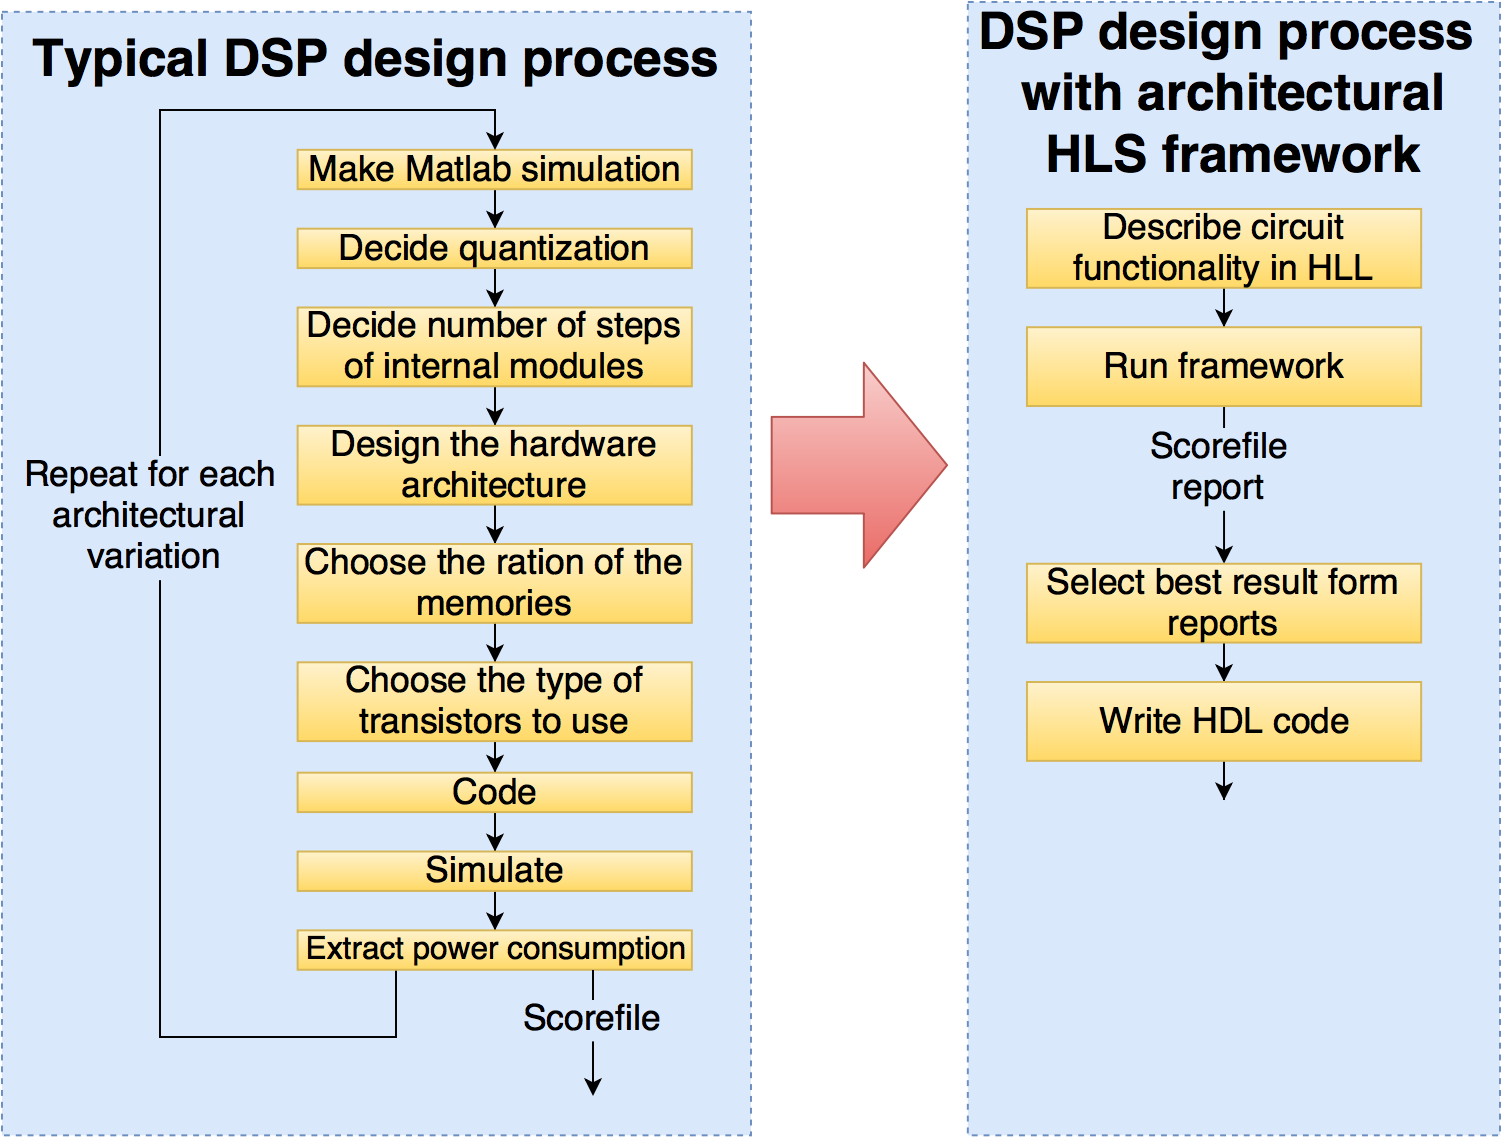
\includegraphics[width=0.75\textwidth]{../figs/Motivation.png}
\caption{\label{fig:motivationflow}Typical DSP design process compared to HLS-framework.}
\end{figure}

The thesis will look at the implementation of a framework for architectural exploration of digital hardware, targeted for \gls{asic} implementation. The ultimate goal is to create a framework that automatically explores a wide variety of architectural variations and presents the best alternatives with regards to a given design goal or constraints.
\section{Previous work}
In my specialization project \cite{holm2015pro}, conducted during the autumn of 2015, I explored the academic open source \gls{hls}-tool \textit{LegUp}. This tool has a maturity not before seen in an academic \gls{hls}-tool, and that it is open-source makes it appealing for the concept of a framework for architectural exploration of hardware. LegUp provides ANSI-C to Verilog high-level synthesis, but their focus is targeted towards implementation on \gls{fpga} architectures. The official target support of the output is limited to a few boards from the \gls{fpga} manufacturer Altera, and beta-support for a single board from Xilinx. This thesis will target \gls{asic} implementations. The findings from \cite{holm2015pro} was that there are some issues with the original version of LegUp, limiting its usability for the desired framework. The issues are mainly related to input and output of the generated modules, structure of memory management, and size of signals. A framework for architectural exploration of hardware, using \gls{hls}, was proposed in \cite{holm2015pro}. An illustration showing the tool- and information-flow of the framework is shown in \cref{fig:frameworkflow}.

\begin{figure}[hbpt]
\centering
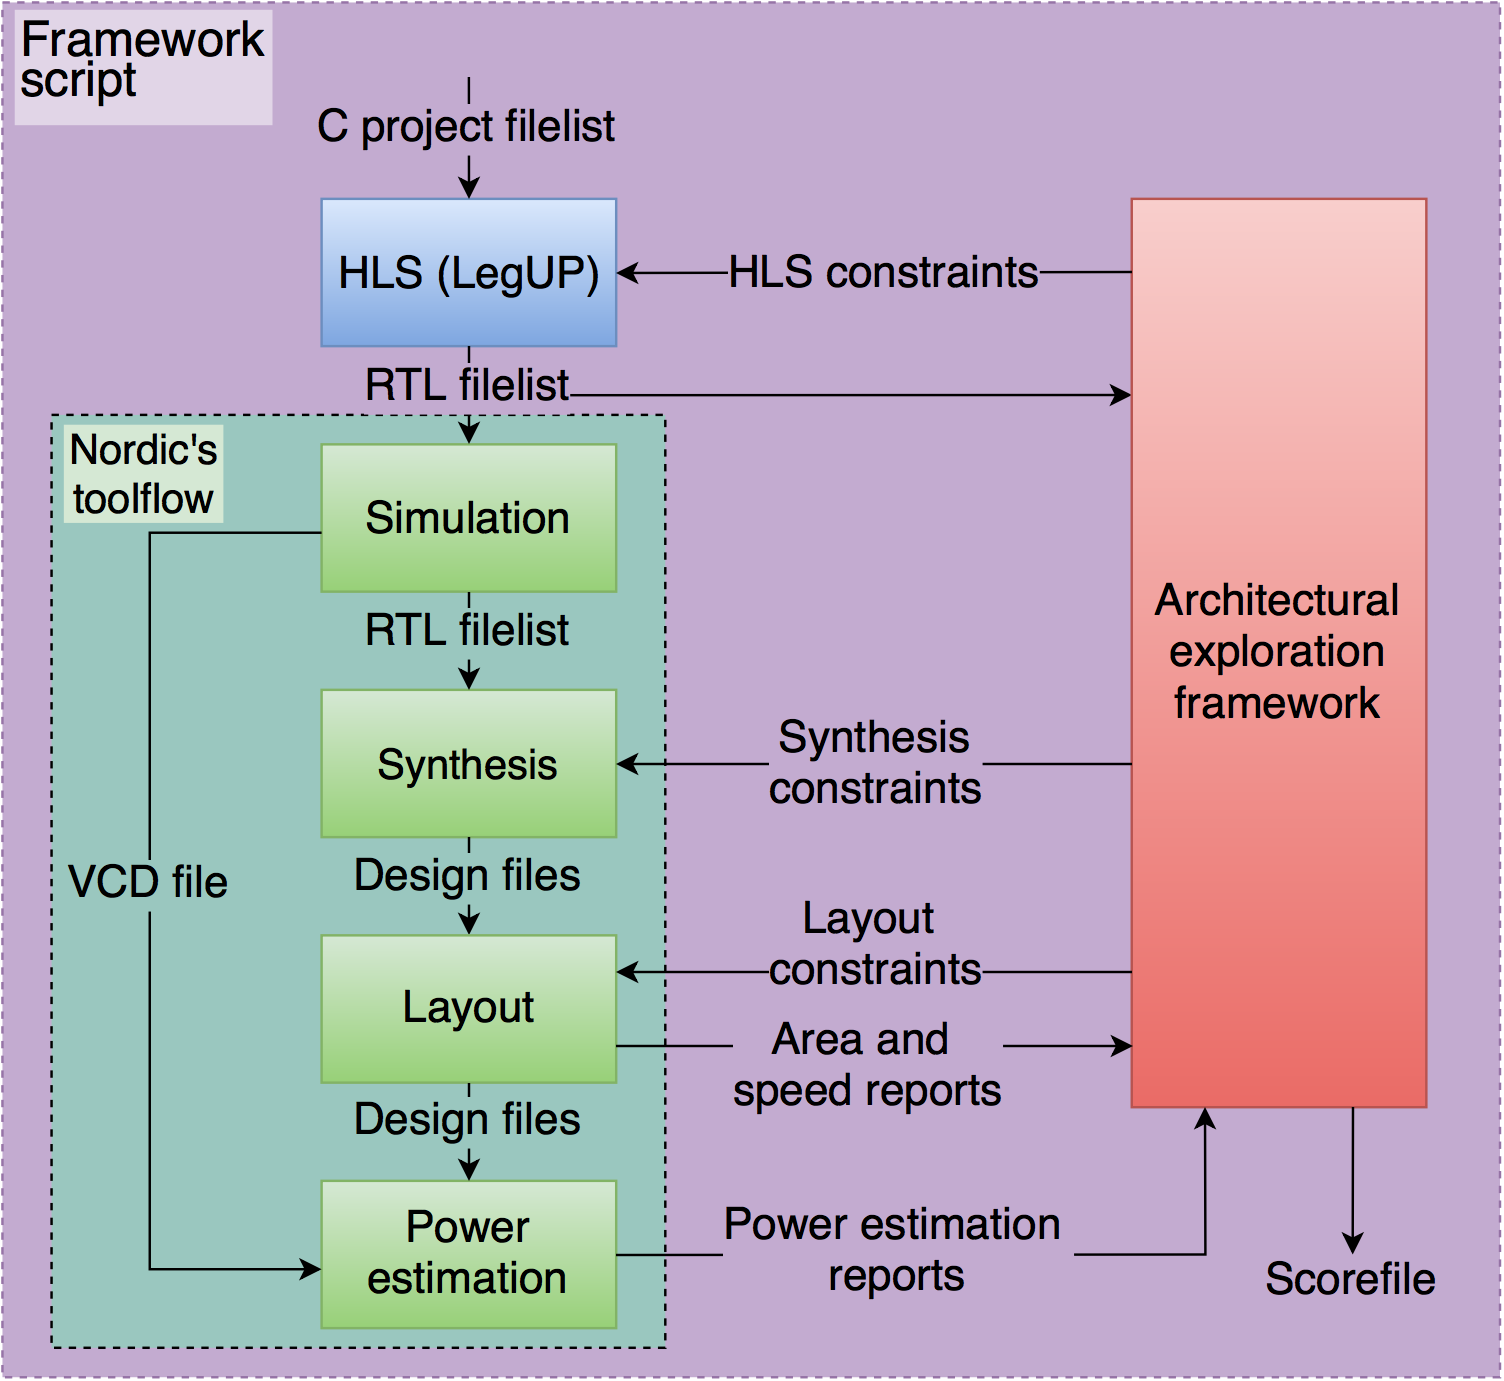
\includegraphics[width=0.75\textwidth]{../figs/Framework.png}
\caption{\label{fig:frameworkflow}Proposed framework-solution \cite{holm2015pro}.}
\end{figure}

\section{\label{sec:projectobj}Project objectives}
The initial goals of the specialization project were found to be a bit exaggerated. For this Master's thesis it was decided to focus on a smaller part of the ultimate goal, to get the necessary basics of the \gls{hls}-tool working well, before proceeding with the framework. The main goal of this thesis is therefore to resolve the issues encountered during the specialization project. It is not know if all issues can be resolved, or how time consuming it will be. Other objectives are therefore added in a prioritized order:

\newcommand\litem[1]{\item{\bfseries #1\\}}
\begin{enumerate}
\litem{Explore approaches} Two possible approaches towards resolving the issued, were described in \cite{holm2015pro}. The first step of this thesis will be to explore both these alternatives and look at positive and negative sides of each method. The outcome of this objective will affect the rest of the work with this thesis, making it an important decision. All aspects of the two approaches must therefore be taken into consideration before making a choice.
\litem{Resolve issues} For LegUp to be usable in a framework for architectural exploration, it is vital that the tool is adapted to generated Verilog suitable for \gls{asic} implementation. This objective is thought to be the most time-consuming, and its outcome is very uncertain. However, if completed successfully, the use-space of LegUp can be extended to other concepts. LegUp’s architecture is, like the input language C, quite memory-bound. \gls{ram} modules, memory controllers, and pointers are used for many things where a simple signal could have given the same result. It should be looked into if this memory-architecture can be changed by de-referencing pointers or turn memory elements into generic signals. A proper way of handling inputs and outputs should also be implemented, to avoid being limited to a certain amount of ports on the generated designs.
\litem{Create framework} When the issues have been resolved, the work with creating a framework for architectural exploration can be started. The framework will be based on the flow shown in \cref{fig:frameworkflow}, using various scripts and programs to run the tool-flow, generating constraints, and creating scorefiles. The framework should be easy to use and ideally be able to run without any interactions with the user.
\litem{Proof of concept} To verify and illustrate the concept in action, a proof of concept will be created. By creating one or more reference designs which will be run through the framework, it is expected to get a wide variety of generated designs with varying results in terms of area, power consumption, and performance. The reference design will also be implemented directly in Verilog \gls{hdl}, to compare and calculate the overhead of the \gls{hls}-generated designs.
\litem{Evaluation} Based on the results from the conducted proof of concept, a re-evaluate of LegUp's usefulness in a framework for architectural exploration of digital hardware, will be conducted. This evaluation will be based on the deviation of the results among the generated designs, as well as the overhead compared to the design written in Verilog. Other aspects can also be considered, like how well the adaption of LegUp is performed and how well the generated Verilog \gls{hdl} synthesize for \gls{asic} architectures.
\litem{Techniques for reducing overhead} The typical overhead of \gls{hls}-tools are in the range of 30-40\%. One of the initial objectives of this concept included the integration of  Nordic Semiconductor's coding style and practices, the \gls{ddvc} \cite{nordicddvc}, into LegUp's Verilog libraries. This include things like interfaces, parameters, naming conventions, power/clock domains, etc. It is assumed that this can give a large reduction of the overhead generated by the \gls{hls}-tool, when integrated into Nordic Semiconductor's existing modules.
\end{enumerate}

\section{Contributions}
The intentions of this work have been to create an adapted version of the open source \gls{hls}-tool LegUp, to make it more suited for generating Verilog targeted towards \gls{asic} architectures. It was also time to create a framework for architectural exploration of digital hardware, and to conduct a proof of concept study.

\textbf{The following list summarize the contributions made through this thesis:}
\begin{itemize}
    \item An adapted version of LegUp has been created. The adapted version support features that is important for implementation towards \gls{asic} architectures. This include the possibility of having multiple inputs and outputs in the generated modules, the inputs and outputs can be streaming, eliminating the need for stopping and starting the module for each run, and an improved method of generating testbenches that include all signals and desired testcases.
    \item A framework for architectural exploration of digital hardware has been developed. This framework can generate a large number of architectural variations with great diversity. Area, power and performance information will automatically be extracted from each design, allowing the designer to choose the best architecture for further implementation.
    \item Using a FIR-filter reference design, a proof of concept study has been conducted, showing that the framework can be used for architectural exploration of digital hardware.
    \item LegUp's usability in a framework for architectural exploration of digital hardware has been evaluated, based on results from the proof of concept study and the performance of the adapted version of LegUp.
\end{itemize}

\section{Method}
The work performed in this thesis is based on multiple research methods. Before the problem could be solved, a study of the architecture and structure of LegUp had to be conducted, to understand the connections and information-flow in the tool. This study was primarily carried out during the previous project \cite{holm2015pro}, but also continued into the work with this thesis. A plan for how to resolve each of the issues at hand was devised and discussed before being carried out, to ensure a good solution. The problems at hand requires in-depth knowledge of the libraries in LegUp, but when the source of the issue had been located, fixing the issue was based on trial and error. By replacing a piece of code with some other solution, a new output can be generated and evaluated. This process is repeated until the issue is resolved. The creation of the framework is based on the idea proposed by Isael Diaz. A study of architectural exploration and \gls{hls}-concepts had to be conducted before building the framework, to make sure the output would have the desired diversity. An experimental study of the usefulness of the created framework was conducted as a proof of concept, to check if the initial hypothesis holds. By running a reference design through the framework, a large amount of data was reported. The data was analyzed to draw the conclusion about the hypothesis.

\section{Overview of the thesis}
In general, this thesis is divided into 8 chapters, each presenting one or more of the project objectives described above, in addition to appendix. In \cref{chp:background}, the background and theory required to understand the rest of the thesis is described. Point one and two from the list above is described in \cref{chp:adaptinglegup}. Chapter \ref{chp:toolflowex} uses a design example to present a thorough description of the information-flow in LegUp and the other tools used in the framework. In \cref{chp:createframework} the third objective, the process of creating a framework, is described. The fourth objective, to create a proof of concept, is presented in \cref{chp:frameworkresults}. The evaluation of the proof of concept results, corresponding to the fifth objective, as well as a discussion of LegUp in general, with focus on its usefulness in the created framework, has been presented in \cref{chp:discussion}. Finally the work is summarized and concluded in \cref{chp:conclusion}. \Cref{chp:conclusion} also include a section of future works, describing aspects that will be interesting to look into more detail at in an eventual continuation of this project. Appendix include code-listings of designs and implementations, that are described and discussed in the main chapters.

\chapter{\label{chp:background}Theory and background}
Theory, background and previous work is important to give a thorough understanding of the material to follow in the next chapters. The base of this background chapter is written as part of the specialization project conducted during the autumn of 2015 \cite{holm2015pro}, but it is included here to allow the report to be a freestanding document. Some sections has been extended to add a deeper level of understanding to some of the described concepts than what were presented in the previous report. Some information from section 3.3 of the \textit{Methodology}-chapter has also been included in \cref{sec:toolflowbg}, as it describes part of the same tool-flow used here.

In the early days of digital hardware design, gate design and layout were performed by hand. With the rapid growth in the numbers of transistors per digital chip-design, this method quickly became too time-consuming and the need for new and more automated design methods rose. \gls{rtl}-design using \gls{hdl} has long been the standard in digital hardware design. With the increasing demand for low power and small area in large \gls{soc} designs with multiple billion transistors, this methodology is no longer sufficient if hardware manufacturers want to hit the window of opportunity with their state-of-the-art product.

\section{\label{sec:hls}High-Level Synthesis}

\gls{hls} is not a new concept as it were introduced in research papers in the late 1970s and further researched and developed in the 1980s and early 1990s \cite{martin2009high}. The available commercial \gls{hls} tools have not been providing the necessary performance and benefits over \gls{hdl} development for major hardware development companies to adapt this methodology until recently.
The concept of \gls{hls} starts with a functional specification of the circuit described using a higher abstraction level, often a \gls{hll}. A tool use target architectural model libraries and design constraints to transform this specification into hardware, represented as a \gls{rtl} or \gls{hdl}-model. The typical \gls{hls}-flow is shown in figure \ref{fig:hlsflow} and each of the transition-steps is described in the below subsections. The input libraries contain information on available hardware resources with power, area, and delay models for the target architecture.

\begin{figure}[hbpt]
\centering
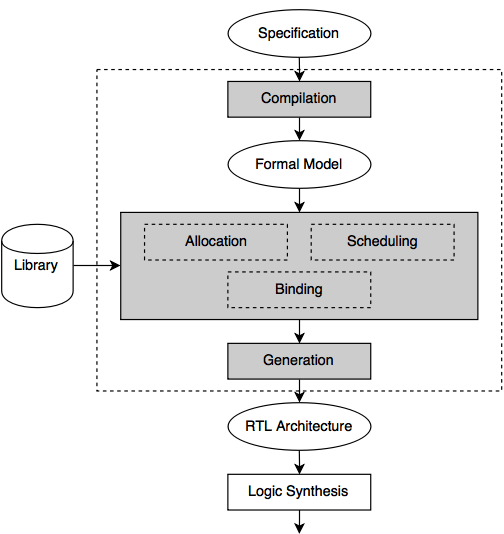
\includegraphics[width=0.55\textwidth]{../figs/HLSFlow.png}
\caption{\label{fig:hlsflow}Information flow in a typical HLS-tool \cite{coussy2009introduction}.}
\end{figure}

\subsubsection{Compilation}

The first step of \gls{hls} is to compile the functional specification into a formal model. This model can vary between different tools, and can be either a specific representation language or a graphic representation of the flow. The formal model is decided by the developers of the \gls{hls} tool. 

\subsubsection{Allocation}

Necessary hardware resources, such as functional units, storage-, and connectivity-components needs to be selected from a given \gls{rtl} component library in order to satisfy the specification and design constraints. Some \gls{hls} tools can also add more resources in the scheduling and binding tasks, if this is needed to meet given constraints.

\subsubsection{Scheduling}
Scheduling arranges all operations in an optimized sequence so that variables are read from sources and brought to the input of the correct functional unit for execution and to the destination afterwards. The scheduler takes all dependencies into account when scheduling the operations, in order to get the most efficient result, as some operations can be executed in parallel if no dependencies exist and there is available resources. Operations can be scheduled to finish in one, or take multiple clock-cycles, and operations can also be chained to eliminate the need for storing the result between operations, and to reduce the total number of cycles needed. 
\subsubsection{Binding}
In the binding task, all clock-cycle-crossing variables, operations, and transfers are bound to a free resource, in the time-frame when it is scheduled. Non-overlapping or mutually exclusive variables can be bound to the the same storage unit, and operations can be bound to the best optimized functional unit if multiple alternatives are available. Each transfer from component to component, either storage or functional unit, needs to be bound to a connection unit, such as a bus or a multiplexer.
\subsubsection{RTL Generation}
The generated \gls{rtl} usually consists of two parts, a control-unit and a data-path-unit. The control-unit is often implemented as a \gls{fsm}, which set control-signals to the data-path, and controls the current and next-state of the system. The data-path contains storage-, functional-, and connection-units. An example of this division is shown in \cref{fig:hlsrtl}.
\begin{figure}[hbpt]
\centering
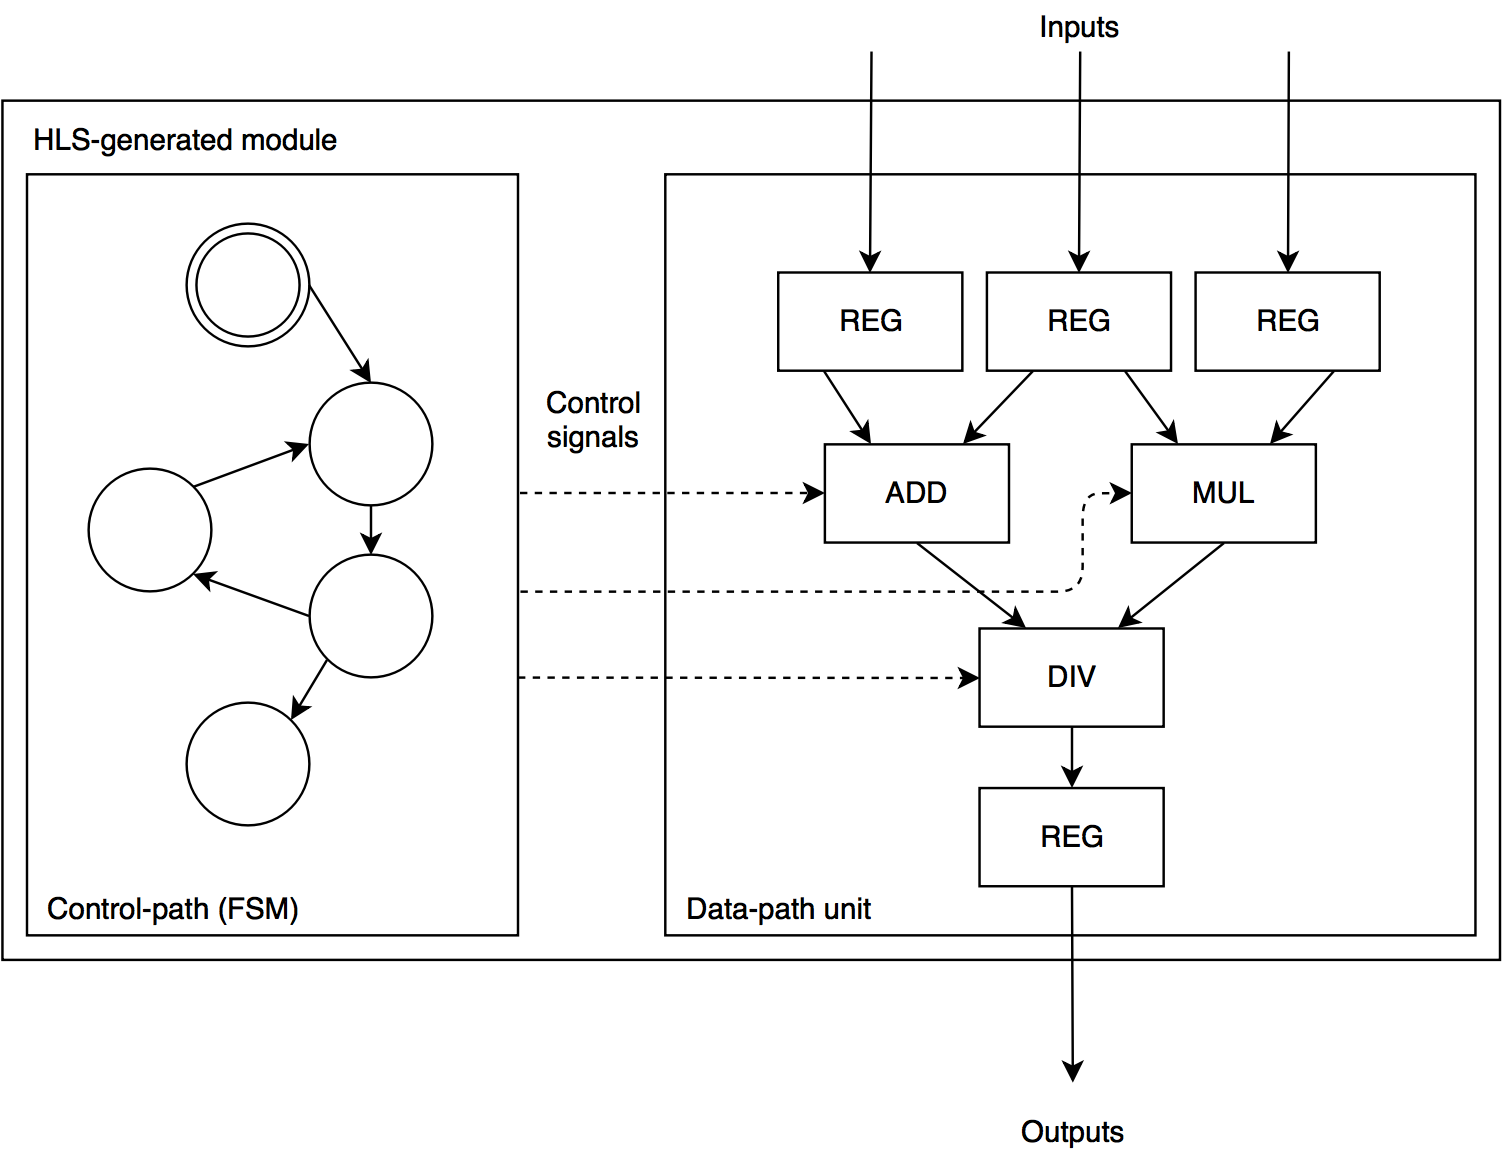
\includegraphics[width=0.65\textwidth]{../figs/HLSRTL.png}
\caption{\label{fig:hlsrtl}Typical division of control and data-path in the generated \gls{rtl} from \gls{hls}.}
\end{figure}
Depending on the intensiveness of the binding step, the output \gls{rtl} can be tightly or loosely bound to the available resources. If an operation is not bound to a specific unit, it is up to the following logic synthesis of the \gls{rtl} to bind the operations to available resources. The different types of \gls{rtl} output are illustrated by the following example. \textit{a = b * c} executing in state \textit{n}:

\begin{minipage}[t][300px]{\textwidth}
\textbf{Without any binding:}%\hfill\vspace{-\baselineskip}
\begin{verbatim}
state (n): a = b * c;
go to state (n + 1);
\end{verbatim}
\textbf{With storage binding:}%\hfill\vspace{-\baselineskip}
\begin{verbatim}
state (n): S(1) = S(2) * S(3);
go to state (n + 1);
\end{verbatim}
\textbf{With functional-unit binding:}%\hfill\vspace{-\baselineskip}
\begin{verbatim}
state (n): a = MUL1 (b, c);
go to state (n + 1);
\end{verbatim}
\textbf{With storage and functional-unit binding:}%\hfill\vspace{-\baselineskip}
\begin{verbatim}
state (n): S(1)=MUL1 (S(2), S(3));
go to state (n + 1);
\end{verbatim}
\textbf{With storage, functional-unit, and connectivity binding:}%\hfill\vspace{-\baselineskip}
\begin{verbatim}
state (n): BUS1 = S(2); BUS2 = S(3);
BUS3 = MUL1 (BUS1, BUS2);
S(1) = BUS3;
go to state (n + 1);
\end{verbatim}
\end{minipage}

A loosely bound \gls{rtl} gives the synthesis-tool the flexibility to optimize the unit binding to updated timing estimates, delays, and loads given by the layout and floor-planning tools.

\section{LegUp}
The \gls{hls} tool used in this project is called LegUp \cite{canis2011legup}. LegUp is an open-source academic tool developed at the University of Toronto, Canada. LegUp's goal is to \textit{"allow researchers to experiment with new \gls{hls} algorithms without building a new infrastructure from scratch"} and their long-term vision is to \textit{"make \gls{fpga} programming easier for software developers"}. LegUp takes \gls{ansi}-C as input and generates synthesizable Verilog \gls{hdl} as output. The developers of LegUp have primarily focused on support for a variety of \gls{fpga} boards from manufacturer Altera, but in the latest version (4.0), beta support for Xilinx devices and possibility to configure the tool to generate generic Verilog to target other \gls{fpga} vendors or even \gls{asic} through use of generic dividers, has been introduced. The big advantage of LegUp compared to similar, commercial tools, is that it is open-source and therefore can be configured to target different architectures. The \gls{rtl} and \gls{hdl} generating part of the tool can be modified or replaced to fit the programmers needs.
Since LegUp, in its unmodified form, target \gls{fpga} devices, it support three different synthesis flows; pure-\gls{sw}, hybrid, and pure-\gls{hw}. The two first synthesis flows will implement a TigerMIPS \cite{tigmips} soft processor, which will run part of the C code. The partitioning of \gls{sw} and \gls{hw} in the individual modules are described in \cref{tab:legupflows}. It is the pure-\gls{hw} flow that will be the focus of this project.

\begin{table}[hbpt]
    \centering
    \caption{\label{tab:legupflows}HLS-flows supported by LegUp and partitioning between SW and HW}
    \begin{tabular}{lp{4.8cm}p{4.8cm}}
      \textbf{Flow} & \textbf{Functions run in hardware} & \textbf{Functions run in software}\\
      \toprule
      Pure-SW & None & All \\
      \hline
      Hybrid & Specified hardware-accelerated functions & All other functions \\
      \hline
      Pure-HW & All & None\\
      \bottomrule
    \end{tabular}
\end{table}

\subsection{Producing Verilog Output}
LegUp is made up of two components; a frontend pass and a target backend pass to the LLVM compiler infrastructure. 
The information flow in LegUp, shown in figure \ref{fig:legupflow}, follows the same principle as the information flow described in section \ref{sec:hls}.
\begin{figure}[hbpt]
\centering
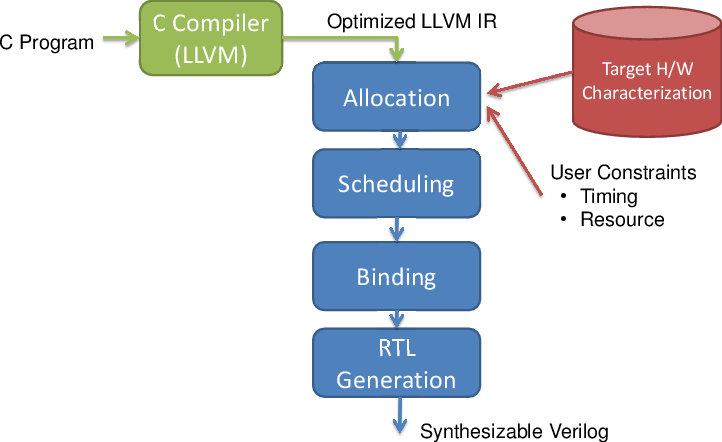
\includegraphics[width=0.6\textwidth]{../figs/LegUpFlow.png}
\caption{\label{fig:legupflow}Information flow in LegUp \cite{legupmaual}.}
\end{figure}
The LegUp LLVM frontend takes LLVM-\gls{ir} compiled by clang, a C frontend for LLVM, as input and links in custom written functions like memcpy, memset and memmove, which do not exist in hardware, but that LLVM assumes exist in the C library. 
The LegUp backend pass performs allocation, scheduling and binding as described in section \ref{sec:hls}. In the next step, \gls{rtl}-module objects that represents the final hardware circuit are generated from each LLVM instruction. Ultimately, Verilog code corresponding to each of the \gls{rtl}-modules is output to a file.

The allocation, scheduling, and binding in LegUp is performed based on information about available resources and timing information about the specified target FPGA-board, in addition to user-defined constraints and setting. The available information about the FPGA-boards allows for precise scheduling and binding to the available resources. Since the implementation of ASIC designs are quite different from the architecture and implementation of designs on FPGAs, the resource and timing information will not be as easily obtained for the target architecture. 

\subsection{\label{sec:legupclasses}Classes}
LegUp has some predefined classes that is important for the understanding of the description of how LegUp is adapted for generating more ASIC compliant Verilog. The following subsections will describe these classes in more detail.
\subsubsection{RTLModule}
The RTLModule class models a hardware RTL module. The class stores information about all ports (inputs and outputs), signals, parameters and sub-modules. Each function declared in the C-code transforms into a RTLModule object. Each function that is called from the function will be added as a sub-module to the RTLModule object, meaning a module instantiation will be added to the module. Important member functions in the RTLModule class is:
\begin{compactdesc}
    \item[getName()] \hfill \\
    Returns a string containing the name of the RTLModule, i.e. "main" for the module generated by the main-function in the C-program.
    \item[find(std::string signal)] \hfill \\
    Takes a string containing a signal name as parameter and returns a pointer to the RTLSignal in the RTLModule with that name.
    \item[addParam()] \hfill \\
    Adds a parameter to the module. The function returns a pointer to the generated RTLSignal object.
    \item[addIn()] \hfill \\
    Adds an input port to the module. The function returns a pointer to the generated RTLSignal object.
    \item[addOut()] \hfill \\
    Adds an output port to the module. The function returns a pointer to the generated RTLSignal object.
    \item[addRegOut()] \hfill \\
    Adds a registered output port to the module. The function returns a pointer to the generated RTLSignal object.
    \item[addReg()] \hfill \\
    Adds a register signal to the module. The function returns a pointer to the generated RTLSignal object.
    \item[addWire()] \hfill \\
    Adds a wire signal to the module. The function returns a pointer to the generated RTLSignal object.
    \item[addModule()] \hfill \\
    Adds a instantiation of another module to the module. The function returns a pointer to the generated RTLModule
    object.
\end{compactdesc}
\subsubsection{RTLSignal}
The RTLSignal class represents the signals within an RTLModule. Both internal signals, port signals and condition signals are all modelled usign the RTLSignal class. Important member functions of the class is:
\begin{compactdesc}
    \item[getName()] \hfill \\
    Returns a string containing the name of the RTLSignal, i.e. "clk" for the clock signal.
    \item[getType()] \hfill \\
    Returns a string describing the signal type. The type can be reg, wire, input, output and output reg.
    \item[getNumDrivers()] \hfill \\
    Return the number of driving RTLSignals. 
    \item[getDriver(unsigned i)] \hfill \\
    Returns a pointer to the i-th driving RTLSignal.
    \item[getCondition(unsigned i)] \hfill \\
    Returns a pointer to the condition signal of the i-th driving RTLSignal.
    \item[addCondition(RTLSignal *cond, RTLSignal *driver)] \hfill \\
    Adds a conditional driver. If the RTLSignal \textit{cond} is true, the RTLSignal \textit{driver} drives the signal. 
    \item[connect(RTLSignal *s)] \hfill \\
    Connect this signal unconditionally to another RTLSignal.
    \item[getWidth()] \hfill \\
    Returns a pointer to a RTLWidth object, describing the width of the RTLSignal.
    \item[isOp()] \hfill \\
    Returns true if the RTLSignal is an RTLOp object.
\end{compactdesc}
\subsubsection{RTLOp}
The RTLOp class is a subclass of the RTLSignal class, representing an operation with one, two or three operands. Each operand is a RTLSignal. The operation can be an arithmetic operation like addition, subtraction, multiplication, or division, and it can also be logical operations like AND, OR, and XOR, or even comparison operations like equal, not equal, less than, less than or equal, greater than, and greater than or equal. The whole list can be seen in the class reference \cite{rtlopclassref}. A RTLOp object modelleing an AND operation of two operands, operand1 and operand2, will in Verilog correspond to the operation \verb!operand1 & operand2!. Some important member functions are:
\begin{compactdesc}
    \item[getOperand(int i)] \hfill \\
    Returns a pointer to i-th operand of the RTLOp object.
    \item[getNumOperands()] \hfill \\
    Returns the number of operands of the RTLOp object.
    \item[setOperand(int i, RTLSignal *s)] \hfill \\
    Sets the i-th operand to the RTLSignal \textit{s}.
\end{compactdesc}
\subsubsection{RTLWidth}
The RTLWidth class represents the bitwidth of a RTLSignal. An RTLWidth is defined by high and low bits, for instance 31,0 for a 32 bit signal. This will transform into \verb![31:0]! in Verilog.
\subsubsection{RAM}
The RAM class models RAM modules in LegUp. Whenever a variable is loaded or stored, a RAM module is generated to handle the loads and stores. The RAM objects can be divided into two scopes; LOCAL and GLOBAL. A Local RAM object is local to a given function and cannot be accessed from other functions. A global RAM object will be implemented in a global memory controller, and all modules that use the variable can connect to the RAM via the memory controller. Some important member functions are:
\begin{compactdesc}
    \item[getName()] \hfill \\
    Returns a string containing the name of the RAM module, i.e. "main\_0\_1" for the RAM module generated for the first parameter to the main function declared as volatile (output parameters) in the C-code.
    \item[isROM()] \hfill \\
    Returns true if the RAM is read-only.
    \item[getScope()] \hfill \\
    Returns if the RAM is in the local or global scope.
\end{compactdesc}


\subsection{Constraints}
Constraints is a important part of LegUp and its usage in this project. The constraints are used for setting design goals and limitations on design, and to specify how the \gls{hls}-flow shall be executed. All available constraints are described in the constraint manual \cite{legupconst}, but the ones used in this project are described in \cref{tab:constraintssescription}. Constraints play an important role in this concept, as the idea is to generate multiple designs that can be compared in terms of area and power consumption. For the designs to be different, varying constraints are used for generating the designs. Some constraints are considered \textit{required}, as they must be set for the generated design to be compatible with the tool-flow. HLS constraints are used for getting different Verilog output from LegUp. Other constraints from the constraint manual can be also be used, but these were selected for this project as their description signalize possibility to affecting the output.
\begin{table}[hbtp]
    \centering
    \begin{tabular}{l|p{6.4cm}|c}
    \multicolumn{3}{c}{\textbf{Required constraints}} \\
    \toprule
    \multicolumn{1}{c}{\textbf{Parameter name}} & \multicolumn{1}{c}{\textbf{Description}} & \specialcell{\textbf{Required}\\\textbf{value}} \\
    \midrule
    \small{DIVIDER\_MODULE} & Use generic divider module rather than Altera primitive & \textit{generic} \\
    \hline
    \specialcelll{\small{EXPLICIT\_}\\\small{LPM\_MULTS}} & Use Altera primitive multiplier rather than Verilog multiply operator (*) & \textit{0} \\
    \hline
    \small{INFERRED\_RAMS} & Use Verilog inferred RAMs rather than Altera altsyncram modules & \textit{1} \\
    \hline
    \specialcelll[t]{\small{INFERRED\_}\\\small{RAM\_FORMAT}} & Select format of inferred RAMs. Altera: multiple always blocks, Xilinx: same always block & \textit{xilinx} \\
    \hline
    \small{LOCAL\_RAMS} & Infer all RAMs as local RAMs rather than global RAMs. RAMs being accessed by multiple functions will override this setting & \textit{1} \\
    \hline
    \small{VSIM\_NO\_ASSERT} & Disable triple-equality assertions. This causes simulation to fail & \textit{1} \\
    \midrule
    \multicolumn{3}{c}{\textbf{HLS constraints}} \\
    \toprule
    \multicolumn{1}{c}{\textbf{Parameter name}} & \multicolumn{2}{c}{\textbf{Description}} \\
    \midrule
    \small{SDC\_NO\_CHAINING} & \multicolumn{2}{p{8cm}}{Schedule each operations into a separate clock cycle} \\
    \hline
    \small{MB\_MINIMIZE\_HW} & \multicolumn{2}{p{8cm}}{Run LegUp-pass that tries to minimize signal sizes} \\
    \hline
    \small{CASE\_FSM} & \multicolumn{2}{p{8cm}}{Use case-statements in FSM rather than If-Else} \\
    \hline
    \small{PIPELINE\_ALL} & \multicolumn{2}{p{8cm}}{Enable pipelining for all loops, regardless of loop-label} \\
    \hline
    \specialcelll{\small{ENABLE\_}\\\small{PATTERN\_SHARING}} & \multicolumn{2}{p{8cm}}{Turn on resource sharing for patterns in \gls{dfg}} \\
    \hline
    \specialcelll{\small{DUAL\_PORT\_}\\\small{BINDING}} & \multicolumn{2}{p{8cm}}{Use dual-ported on-chip memories} \\
    \bottomrule
    \end{tabular}
    \caption{Descriptions of constraints used in this project}
    \label{tab:constraintssescription}
\end{table}

\section{\label{sec:LLVM}LLVM}
LLVM \cite{LLVM:CGO04}, formerly Low-Level Virtual Machine, is a compiler framework that was originally developed as a research infrastructure to investigate dynamic compilation techniques for static and dynamic programming languages, at the University of Illinois in 2000. It is now a open-source project with many contributors from both industry, research groups and individuals, and it is used by companies like Apple in their Xcode \gls{ide} \cite{llvmapple} and Sony for their PS4 developer toolchain \cite{llvmsony}. LLVM support a large number of frontends for programming languages, including Clang \cite{clang} which support C, C++, Obcjective-C, and Objective-C++, and is compatible with \gls{gcc}. It also supports a large number of backend target architectures. Figure \ref{fig:llvmcompiler} shows how different source languages can be input to the frontend compilers of LLVM, which translate the source into an \gls{ir}. The \gls{ir} is then optimized using LLVM's optimizer. At this stage, different source languages can be linked together, and even object files compiled using standard \gls{gcc} can be linked at this stage. The optimized \gls{ir} is then translated into the target architecture by the backend.

\begin{figure}[hbpt]
\centering
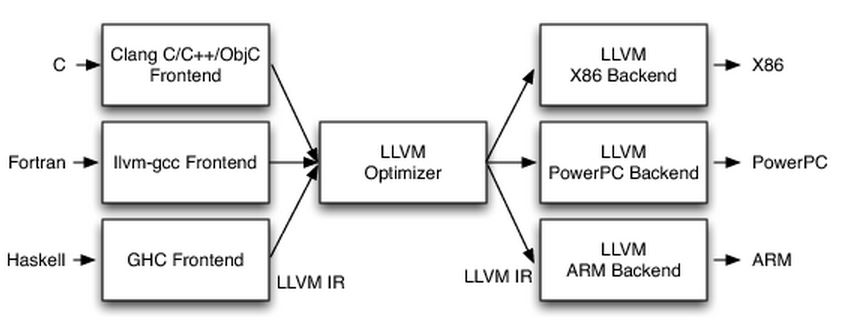
\includegraphics[width=\textwidth]{../figs/LLVMCompiler.jpg}
\caption{\label{fig:llvmcompiler}LLVM's three-phase compiler structure \cite{llvmarch}.}
\end{figure}

\subsection{Intermediate Representation}
LLVM use a human readable assembly-like, strongly typed RISC instruction set as their \gls{ir}, with support for an infinite number of temporary registers of the form \%0, \%1, etc. LLVM-\gls{ir} can also output a dense bitcode format for serialization. Conversion between the bitcode-format and the human-readable format, and vice versa, can be done with the commands "\verb!llvm-dis!" and "\verb!llvm-as!", for dis-assembly and assembly.

Some parts of the LLVM \gls{ir} will be described in \cref{chp:toolflowex}. The whole language are too large to be fully explained here, but interested readers can read more about the syntax in the \textit{LLVM Language Reference Manual} \cite{llvmlangman}.

\section{Alternative hardware design methods}
\gls{hls} is not the only alternative to \gls{hdl}-languages, if you want to design digital hardware at a higher level of abstraction. The following subsections will shortly describe two alternative approaches to digital hardware design. 
\subsection{Chisel}
One interesting approach to designing hardware with a higher level of abstraction, is the Chisel \gls{hcl} \cite{bachrach2012chisel}, developed at UC Berkeley. Unlike \gls{hdl} languages like VHDL and Verilog, which were originally designed as simulation languages and later adopted as a basic for synthesis, Chisel was created as a \gls{hcl} and is thus \textit{synthesizable by construction}. This entails that no conversion from C, or other \gls{hll}, into gates is performed, only generation of generic low-level Verilog with no overhead. Chisel is a \gls{dsl} built on Scala \cite{odersky2004overview} with its own syntax, but Scala syntax can also be used to get even greater abstraction in your design. A big advantage using Chisel is its high simulation speed, using C++-based cycle-accurate software simulators.

\subsection{Functional programming}
Functional programming is a relatively different method of hardware design, as it consists only of mathematical functions and immutable data. Two examples of hardware design using functional programming is C$\lambda$aSH \cite{baaij2009clash} and Lava \cite{bjesse1998lava}. Both Lava and C$\lambda$ash are compilers for the functional programming language Haskell \cite{haskellonline}, but while Lava is an embedded \gls{dsl} like Chisel, with its own syntax, C$\lambda$ash use Haskell syntax and semantics, and use a static analysis approach towards synthesis.

\section{Programming concepts}
In high-level programming languages like C and C++ and in \gls{hdl} languages like Verilog, the use of programming concepts are extensively used. This section describes some concepts that are frequently referred throughout this report.
\subsection{Structures}
A structure, or struct for short, is a complex data-type that can contain multiple other variables of different data-types. 
\subsection{Classes}
A class can contain multiple variables of different data-types, like a struct, but in addition a class can have member.functions and divide its member into a public and a private scope. The private members of a class can only be accessed through public member-functions. This added level of security increase the level of integrity of the objects.
\subsection{Pointers}
A pointer is a variable that is defined to point at a location in memory where another object is stores. The pointer itself contains the memory address of the object it points at.
\subsection{Declaration}
Declaration refers to the process of declaring a type or an object that will be used at a later stage. This can for instance be be a struct in C, a class in C++ or a module in Verilog. A type or an object, needs only to be declared once and can then be used as many times as necessary. An example of a declaration of a struct in C: 
\lstset{language=C++, style=Cstyle}
\begin{lstlisting}
struct Book { char title[128], 
              char author[128], 
              int isbn 
            } ;
\end{lstlisting}
\subsection{Instantiation}
Instantiation is when the object you created with your declaration, is created and stored at a designated location in memory. When you instantiate an object, you usually assigns it a variable, or name, that you use throughout the scope of the object to reference the object. In Verilog we often talk about module \textit{instantiation}. This is the same concept as in \gls{hll}-languages, but here a declared module is placed inside another module, making it a \textit{sub-module}.
\subsection{Assignment}
Assignment is when you give an instantiated object a value, i.e. you are assigning a value to the object.
\subsection{Defining types}
A user-defined structure or object can be defined as a type in C. The struct-example from above can be defined as a type by the line:
\begin{lstlisting}
typedef struct Book Book_t
\end{lstlisting}
Now an object of the type \textit{struct Book} can be instantiated using the line:

\verb!Book_t mybook!,

where \textit{mybook} is the variable name. Using \textit{typedef} saves time and reduce code-size in many cases.

\section{\label{sec:powdiss}Power dissipation in CMOS circuits}
The power dissipation in CMOS circuits can be divided into three categories \cite{panda2010power}, \textit{dynamic power}, \textit{short-circuit power} and \textit{leakage power}. This gives a total power dissipation of:
\begin{equation}
    P_{total} = P_{dynamic} + P_{short-circuit} + P_{leakage}
\end{equation}

Figure \cref{fig:powerdisscmos} shows the distribution of the power components of the CMOS circuit. Each component is described in more detail in the following subsections, where \textit{switching power} corresponds to $P_{dynamic}$, \textit{internal power} corresponds to $P_{short-curcuit}$, and \textit{leakage power} to $P_{leakage}$.
\begin{figure}[hbpt]
\centering
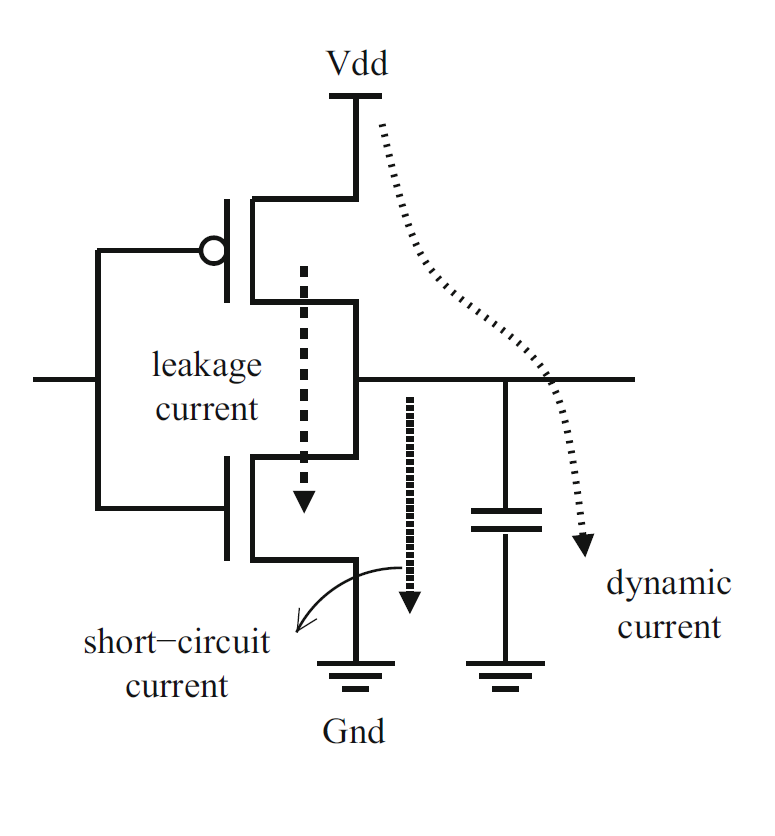
\includegraphics[width=0.4\textwidth]{../figs/PowerDissipation.png}
\caption{\label{fig:powerdisscmos}Power dissipation components distribution \cite{panda2010power}.}
\end{figure}

\subsection{Switching power}
\textit{Switching power} arise whenever a signal change the logic state from 0 to 1, causing the load capacitance to be charged by the power supply. Half the energy drawn from the power supply needed to charge the capacitance, is dissipated as heat in the process. The \textit{switching power} depends on the frequency of the switching, the switching factor of gates and the load capacitance in addition to the supply voltage. 

\subsection{Internal power}
The \textit{internal power} is the power used to charge and discharge the internal capacitance of the circuits whenever a pin change its state. A large part of the \textit{internal power} is the short-circuit power. In the short time when both the pMOS and nMOS transistor of the CMOS circuit is \textit{on}, a current will be drawn from the source $V_{dd}$ to ground through the short-circuit that will occur. 

\subsection{Leakage power}
Whenever the circuits are turned \textit{on}, a small leakage current will be drawn from the gates. The leakage power is mostly caused by sub-threshold currents and reverse biased diodes in the circuits. The leakage current increase when the technology shrinks, making leakage a bigger problem today than before. 

\section{\label{sec:toolflowbg}Tool-flow}
This tool-flow section will describe all the tools that are used throughout this thesis, and the connection and data-flow between the different tools. This flow is based on the standard tool-flow used at Nordic Semiconductor, as well as some parts adapted from the "\textit{automated area and power estimation tool-flow}" created by Joar Talstad for his Master thesis \cite{talstad15master}. Most of the tool-flow is based on scripts and Makefiles that can be run from a Linux shell, but there are also some GUI-tools available that will be mentioned briefly in \cref{chp:toolflowex}. The following subsection will describe the different sections of the tool-flow in detail. The flow in LegUp will not be described here, as this is covered above and will be presented in more detail in \cref{chp:toolflowex}.

\subsection{Simulation}
Simulation is run to verify the correctness of a design and to help detect and eliminate potential bugs. In this project, the simulation tool also generates a \gls{vcd}-file, showing switching activity during simulation. This file is used in the power analysis tool later in the flow, to get a realistic input of the amount of switching in the design. Simulation is performed using the tool ModelSim for Questa-64, version 10.2b 2013.05 \cite{questasim}. Simulation is executed by calling the script \textit{RUN\_ALL}. The \gls{rtl}-design filelist and a file containing a testbench module must be specified in the filelist found in the \textit{sim/tb/}-directory, at this is used as input to the simulation tool.
\subsection{Synthesis}
Synthesis translates a \gls{rtl}-design written in a \gls{hdl}-language, like Verilog or VHDL, into a netlist for a specified target library. The tool used for synthesis in this project is Synopsys Design Compiler, version I-2013.12-SP2 \cite{syndescomp}. A cell library describing 180nm technology is used as the target architecture. A Makefile is used to start synthesis, and the command \verb!make compile! runs the full synthesis. The netlist generated by synthesis is found in the file \textit{designName.mapped.v} in the \textit{result}-directory. This netlist is used as input for the layout-tool. Synthesis generated reports showing area-estimates, register count, critical path and static power estimates for the design. As the design will be processed further through the tool-flow, these reports are not that accurate or useful.
\subsection{Layout}
Layout translates the netlist generated during synthesis into a chip layout. The tool used for layout in this project is Synopsys IC Compiler, version L-2016.03-SP1 \cite{syniccomp}. A Makefile is used to start layout, and the command \verb!make outputs_cts! runs the correct layout-script. Layout produces a new netlist-file, stored in the file \textit{designName.output.v} in the \textit{result}-directory. This netlist is used in the power analysis tool for estimating power consumption. From layout, reports about area and critical paths are stored in the \textit{reports}-directory. These results are more accurate, as they were gathered from the actual chip layout.
\subsection{\label{sec:powest}Power analysis}
Power analysss is performed to get an early indication on how much power the final design will be consuming. The tool used power analysis in this project is Synopsys Primetime, version K-2015.12-SP3. To get accurate power estimates, the switching activity file generated during simulating is used together with the netlist output from layout. The conclusion from \cite{talstad15master} were that this method is well suited for making RTL-design trade-offs based on power consumption in multi-voltage designs, providing accurate results. Power analysis is run on five different power scenarios, each giving a separate result for each of the three power dissipation categories described in \cref{sec:powdiss}. The reports are stored in the \textit{reports}-directory.

\section{Linux tools}
Some tools available in Linux is used throughout the scripts created in this thesis. The following subsections will give a short introduction to the most important tools and its usage.
\subsection{bash}
\textit{bash} is the default shell, or command language interpreter, in Linux. A shell processes macros and executes commands. By adding commands to a file, i.e. a script, a long list of commands can be executed in order. For a script to be executed in the bash shell, the \textit{shebang}-line, the first line of the file, needs to contain the path to the bash shell. The line \verb!#!/bin/bash! can be used in most cases, but for portability, the line \verb!#!/usr/bin/env bash! is the safest choice.

\subsection{make}
\textit{make} is a tool used to decide which parts of a large program needs to be recompiled. The synopsis of \textit{make} is:

\verb!make [OPTIONS] [TARGETS]!

Some options for make are:\\
\verb!-f MAKEFILE     !\textit{Provide the path to the Makefile}
\verb

To use \textit{make}, a \textit{Makefile} describing the relationships between the files of the program is needed. If the Makefile is present in the folder where you run the \textit{make}-tool, you do not need to specify the path to the file. The Makefile can define multiple targets, each performing a separate compilation. There can be dependencies between the targets, forcing the dependency-targets to be compiled before specified target.
\subsection{grep}
\textit{grep} is used to search for the occurrence of a pattern in a given file, and print each line found. The synopsis of \textit{grep} is:

\verb!grep [OPTIONS] PATTERN [FILE...]!

where PATTERN is the pattern to be matched, and FILE is the path to the file(s) to be searched.

Some important options used with \textit{grep} are:\\
\verb!-e PATTERN      !\textit{Provide multiple patterns}\\
\verb!-f FILE         !\textit{Get PATTERN from file}\\
\verb!-c              !\textit{Return number of matched lines}\\
\verb!-m NUM          !\textit{Exit after NUM matches}

If you run the command "\verb!grep "one"!" on a file containing the following lines:

\verb!one two three!\\
\verb!one!\\
\verb!two!

the output will be:

\verb!one two three!\\
\verb!two!

as the first and the last line of the input contains the pattern \textit{two}.

\subsection{Substring replacement}

As \textit{grep} returns the whole line that were matched we need a way to eliminate unwanted information from the returned line. For this purpose, the tool \textit{sed} could be used, but when using the \textit{bash}-shell for scripts, a similar tool called substring replacement is included natively. The syntax of substring replacement is:

\verb!\${string/substring/replacement}!

where \textit{string} is a string, \textit{substring} is the text to be replaced and \textit{replacement} is the string that \textit{substring} will be replaced with. Notice that \textit{string} can be both a literate string and a variable containing a string, depending on the use. This format will only replace the first occurrence of \textit{substring} on each line of \textit{string}. To replace all occurrences, this format must be used:

\verb!\${string//substring/replacement}!

If the command "\verb!${"one two one two"//one/three}!" is run, the output would give \verb!"three two three two"!, as all occurrences of the substring \textit{one} will be replaced by \textit{three}.

\section{Reference design}
\label{sec:refdes}
This thesis will look into whether or not LegUp can be used as the HLS-tool in a framework for architectural exploration of hardware. In order to get some output from LegUp than can be compared towards each other, a reference design must be created. The design must be something that can be implemented both in C and Verilog and it should be easy to implement. In \cite{holm2015pro}, two reference designs were implemented; a FIR-filter and a SAP-1 architecture. The FIR-filter will be used as the reference design in this project, as this is a regular structure that easily can be implemented and verified. The SAP-1 architecture would have been a interesting second reference design, as it consists of a FSM, just like the output from LegUp. Unfortunately, this architecture has too many design-parts that makes it hard to write a functional specification for it in C.

\subsection{\label{subsec:refdesfir}FIR-filter}
\gls{fir}-filters are together with \gls{iir}-filters, the two categories of linear time-invariant systems, used in digital signal processing application. The impulse response of a \gls{fir}-filter is zero outside some finite time interval. 
A general \gls{fir}-filter can be described by the differential equation \cite{proakis2007digital}:
\begin{equation}
    y(n)=\sum\limits_{k=0}^{M-1} b_kx(n-k)
    \label{eq:firfilterdiff}
\end{equation}
or by the system function:
\begin{equation}
    H(z)=\sum\limits_{n=0}^{M-1} b_nz^{-n}
    \label{eq:firfiltersys}
\end{equation}
The impulse response for a \gls{fir}-filter is given by:
\begin{equation}
    h(n)\triangleq
    \begin{cases}
    \begin{tabular}{ll}
      $0,$ & $n < 0$  \\
      $b_n,$ & $0 \leq n \leq M-1$  \\
      $0,$ & $n > M$   
      \end{tabular}
    \end{cases}
    \label{eq:firfilterimp}
\end{equation}
From \cref{eq:firfilterdiff} and \cref{eq:firfilterimp} we get the discrete convolution equation:
\begin{equation}
    y(n)=\sum\limits_{k=-\infty}^{\infty} h(k)x(n-k) \triangleq h(n) \ast x(n)
    \label{eq:firfilterconv}
\end{equation}
\noindent
Figure \ref{fig:firfilter} shows the direct form representation of a N-order \gls{fir}-filter with N+1 taps. The figure shows that a FIR-filter requires $N-1$ memory elements, \textit{N} adders and \textit{N} multipliers. 
\begin{figure}[hbpt]
\centering
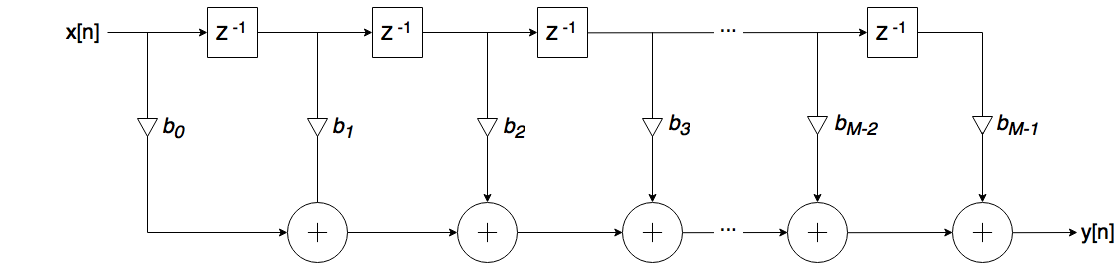
\includegraphics[width=\textwidth]{../figs/FIRFilter.png}
\caption{\label{fig:firfilter}Direct form representation of a N-order FIR-filter.}
\end{figure}


Even though the process of designing a \gls{fir}-filter might not be a trivial task, the implementation of an already designed filter is simple. As seen from \cref{eq:firfilterconv}, the filter can be described by the convolution formula, which implies that the filter can be implemented as convolution of the input function \textit{x(n)} with the impulse response function \textit{h(n)}.
\chapter{Methodology}

\section{\label{sec:legupclasses}LegUp classes}
LegUp has some predefined classes that is important for the understanding of the following description of how the issues in LegUp are resolved. The following subsections will describe these classes in more detail.
\subsection{RTLModule}
The RTLModule class models a hardware RTL module. The class stores information about all ports (inputs and outputs), signals, parameters and sub-modules. Each function declared in the C-code transforms into a RTLModule object. Each function that is called from the function will be added as a sub-module to the RTLModule object, meaning a module instantiation will be added to the module. Important member functions in the RTLModule class is:
\begin{compactdesc}
    \item[getName()] \hfill \\
    Returns a string containing the name of the RTLModule, i.e. "main" for the module generated by the main-function in the C-program.
    \item[find(std::string signal)] \hfill \\
    Takes a string containing a signal name as parameter and returns a pointer to the RTLSignal in the RTLModule with that name.
    \item[addParam()] \hfill \\
    Adds a parameter to the module. The function returns a pointer to the generated RTLSignal object.
    \item[addIn()] \hfill \\
    Adds an input port to the module. The function returns a pointer to the generated RTLSignal object.
    \item[addOut()] \hfill \\
    Adds an output port to the module. The function returns a pointer to the generated RTLSignal object.
    \item[addRegOut()] \hfill \\
    Adds a registered output port to the module. The function returns a pointer to the generated RTLSignal object.
    \item[addReg()] \hfill \\
    Adds a register signal to the module. The function returns a pointer to the generated RTLSignal object.
    \item[addWire()] \hfill \\
    Adds a wire signal to the module. The function returns a pointer to the generated RTLSignal object.
    \item[addModule()] \hfill \\
    Adds a instantiation of another module to the module. The function returns a pointer to the generated RTLModule
    object.
\end{compactdesc}
\subsection{RTLSignal}
The RTLSignal class represents the signals within an RTLModule. Both internal signals, port signals and condition signals are all modelled usign the RTLSignal class. Important member functions of the class is:
\begin{compactdesc}
    \item[getName()] \hfill \\
    Returns a string containing the name of the RTLSignal, i.e. "clk" for the clock signal.
    \item[getType()] \hfill \\
    Returns a string describing the signal type. The type can be reg, wire, input, output and output reg.
    \item[getNumDrivers()] \hfill \\
    Return the number of driving RTLSignals. 
    \item[getDriver(unsigned i)] \hfill \\
    Returns a pointer to the i-th driving RTLSignal.
    \item[getCondition(unsigned i)] \hfill \\
    Returns a pointer to the condition signal of the i-th driving RTLSignal.
    \item[addCondition(RTLSignal *cond, RTLSignal *driver)] \hfill \\
    Adds a conditional driver. If the RTLSignal \textit{cond} is true, the RTLSignal \textit{driver} drives the signal. 
    \item[connect(RTLSignal *s)] \hfill \\
    Connect this signal unconditionally to another RTLSignal.
    \item[getWidth()] \hfill \\
    Returns a pointer to a RTLWidth object, describing the width of the RTLSignal.
    \item[isOp()] \hfill \\
    Returns true if the RTLSignal is an RTLOp object.
\end{compactdesc}
\subsection{RTLOp}
The RTLOp class is a subclass of the RTLSignal class, representing an operation with one, two or three operands. Each operand is a RTLSignal. The operation can be an arithmetic operation like addition, subtraction, multiplication, or division, and it can also be logical operations like AND, OR, and XOR, or even comparison operations like equal, not equal, less than, less than or equal, greater than, and greater than or equal. The whole list can be seen in the class reference \cite{rtlopclassref}. A RTLOp object modelleing an AND operation of two operands, operand1 and operand2, will in Verilog correspond to the operation \verb!operand1 & operand2!. Some important member functions are:
\begin{compactdesc}
    \item[getOperand(int i)] \hfill \\
    Returns a pointer to i-th operand of the RTLOp object.
    \item[getNumOperands()] \hfill \\
    Returns the number of operands of the RTLOp object.
    \item[setOperand(int i, RTLSignal *s)] \hfill \\
    Sets the i-th operand to the RTLSignal \textit{s}.
\end{compactdesc}
\subsection{RTLWidth}
The RTLWidth class represents the bitwidth of a RTLSignal. An RTLWidth is defined by high and low bits, for instance 31,0 for a 32 bit signal. This will transform into \verb![31:0]! in Verilog.
\subsection{RAM}
The RAM class models RAM modules in LegUp. Whenever a variable is loaded or stored, a RAM module is generated to handle the loads and stores. The RAM objects can be divided into two scopes; LOCAL and GLOBAL. A Local RAM object is local to a given function and cannot be accessed from other functions. A global RAM object will be implemented in a global memory controller, and all modules that use the variable can connect to the RAM via the memory controller. Some important member functions are:
\begin{compactdesc}
    \item[getName()] \hfill \\
    Returns a string containing the name of the RTLModule, i.e. "main\_0\_1" for the RAM module generated for the first parameter to the main function declared as volatile (output parameters) in the C-code.
    \item[isROM()] \hfill \\
    Returns true if the RAM is read-only.
    \item[getScope()] \hfill \\
    Returns if the RAM is in the local or global scope.
\end{compactdesc}

\section{LegUp tool-flow example}
To give you a general idea of how LegUp works, this section will give a simple example starting with the C-code and all the way through synthesis and layout. \Cref{lst:ccodelisting} shows a simple C-program with two functions, main and squared. The main function will be the top function and this function takes three input parameters, \textit{done}, \textit{inData} and \textit{\_\_out\_outData}. The main function contains a while loop, which will run as long as the input parameter done is set to zero. Inside the loop the function squared is called with the argument from inData and the return value from squared is assigned to the input argument \textit{\_\_out\_outData}. If you are familiar with C programming, you will see that it is a weird thing to be assigning values to the inputs, but as we will see later in \cref{sec:assValueToOutput}, this is a way to get multiple outputs to the generated module. Notice also the \textit{volatile} keyword in the declaration of the \textit{\_\_out\_outData} parameter, as this is a necessary part of the generating outputs.
\lstset{language=C++,style=Cstyle}
\begin{lstlisting}[caption={Simple C-code example},label=lst:ccodelisting]
int squared (int base) {
  return base * base;
}

int main (int done, int inData, volatile int __out_outData) {
  while(done == 0) {
    __out_outData = squared(inData);
  }
  return 0;
}
\end{lstlisting}

\subsection{HLS with LegUp}
The C-code is compilated into LLVM IR using the clang frontend for the LLVM compilation framework. The initial result before any \gls{lto} is performed is shown in \cref{lst:llvmirprelto}. If you are familiar with assembly code, you might understand some of the operations, like alloca, load, store, mul and icmp. Each define block corresponds to one function from the C-code. The main function, which contains a while-loop, is split into multiple labels. The first section refers to the input parameters and memory allocation and storing of these. Temporary registers, declared on the form \%1, \%2 .. \%N, are inserted where needed. The section from the line "\textit{; <label>:4}" is the checking of the condition of the while loop. Further, \textit{label 7} is operations inside the while loop, and \textit{label 10} is operations after the loop has exited.
\lstset{language=llvm,style=LLVMstyle}
\begin{lstlisting}[caption={LLVM IR before LTO},label=lst:llvmirprelto]
define i32 @squared(i32 %base) #0 {
  %1 = alloca i32, align 4
  store i32 %base, i32* %1, align 4
  %2 = load i32* %1, align 4
  %3 = load i32* %1, align 4
  %4 = mul nsw i32 %2, %3
  ret i32 %4
}

; Function Attrs: noinline nounwind
define i32 @main(i32 %done, i32 %inData, i32 %__out_outData) #0 {
  %1 = alloca i32, align 4
  %2 = alloca i32, align 4
  %3 = alloca i32, align 4
  store i32 %done, i32* %1, align 4
  store i32 %inData, i32* %2, align 4
  store volatile i32 %__out_outData, i32* %3, align 4
  br label %4

; <label>:4                              ; preds = %7, %0
  %5 = load i32* %1, align 4
  %6 = icmp eq i32 %5, 0
  br i1 %6, label %7, label %10

; <label>:7                              ; preds = %4
  %8 = load i32* %2, align 4
  %9 = call i32 @squared(i32 %8) #1
  store volatile i32 %9, i32* %3, align 4
  br label %4

; <label>:10                             ; preds = %4
  ret i32 0
}
\end{lstlisting}
By default, some optimization passes are run on the IR to remove unnecessary operations and reduce the number of registers needed. All available passes are described in \cite{llvmpasses}, but the ones that is run by default is \textit{mem2reg}, \textit{instcombine}, \textit{loops}, \textit{loop-simplify}, \textit{basicaa}, \textit{indvars}, \textit{loop-pipeline}, \textit{internalize}, and \textit{globaldce}. These passes analyses, simplifies and removes operations. The result is listed in \cref{lst:llvmirpostlto}. Notice that the only stores left in the code is the ones connected to the input parameter declared as volatile. The keyword volatile, which definition is \textit{likely to change suddenly and unexpectedly}, tells the compiler to avoid performing optimizations on this object, as it might change in an unexpected way. This is what we want, as assigning values to an input parameter in C does not make sense, and would therefore have been optimized away. 

\begin{lstlisting}[caption={LLVM IR after LTO},label=lst:llvmirpostlto]
define internal i32 @squared(i32 %base) #0 {
  %1 = mul nsw i32 %base, %base
  ret i32 %1
}

; Function Attrs: noinline nounwind
define i32 @main(i32 %done, i32 %inData, i32 %__out_outData) #0 {
  %1 = alloca i32, align 4
  store volatile i32 %__out_outData, i32* %1, align 4
  br label %2

; <label>:2                              ; preds = %4, %0
  %3 = icmp eq i32 %done, 0
  br i1 %3, label %4, label %6

; <label>:4                              ; preds = %2
  %5 = call i32 @squared(i32 %inData) #1
  store volatile i32 %5, i32* %1, align 4
  br label %2

; <label>:6                              ; preds = %2
  ret i32 0
}
\end{lstlisting}

Also notice that the storing and loading of the other input parameters has been swapped by referencing the input parameter register directly. For instance the four lines:

\begin{lstlisting}
%2 = alloca i32, align 4
store i32 %inData, i32* %2, align 4
%8 = load i32* %2, align 4
%9 = call i32 @squared(i32 %8) #1
\end{lstlisting}
has been transformed into the single line:
\begin{lstlisting}
%5 = call i32 @squared(i32 %inData) #1
\end{lstlisting}
The LegUp backend pass for LLVM is run on the IR to generate Verilog-output. LegUp perfomes allocation, scheduling and builds RTL models of the functionality, based on given constraints. These RTL models are printed to a file as Verilog HDL. \cref{lst:verilogmodule1} shows the declaration of the \textit{main}-module, parameters representing states, port and internal signal declarations and instantiation of sub-modules.
\lstset{language=Verilog, style=VerilogStyle}
\begin{lstlisting}[caption={Verilog module, port, signal and parameter declaration, and sub-module instantiation},label=lst:verilogmodule1]
module main
(
	clk,
	clk2x,
	clk1x_follower,
	reset,
	start,
	finish,
	memory_controller_waitrequest,
	return_val,
	arg_done,
	arg_inData,
	arg_outData,
	arg_outData_valid,
	iterationFinish
);

parameter [3:0] LEGUP_0 = 4'd0;
parameter [3:0] LEGUP_F_main_BB__0_1 = 4'd1;
parameter [3:0] LEGUP_F_main_BB__0_2 = 4'd2;
parameter [3:0] LEGUP_F_main_BB__2_3 = 4'd3;
parameter [3:0] LEGUP_F_main_BB__4_4 = 4'd4;
parameter [3:0] LEGUP_F_main_BB__4_6 = 4'd6;
parameter [3:0] LEGUP_F_main_BB__4_7 = 4'd7;
parameter [3:0] LEGUP_F_main_BB__6_8 = 4'd8;
parameter [3:0] LEGUP_function_call_5 = 4'd5;

input  clk;
input  reset;
input  start;
output reg  finish;
input  memory_controller_waitrequest;
output reg [31:0] return_val;
input [31:0] arg_done;
input [31:0] arg_inData;
output reg [31:0] arg_outData;
output reg  arg_outData_valid;
output reg  iterationFinish;
reg [3:0] cur_state;
reg [3:0] next_state;

squared squared (
	.memory_controller_waitrequest (memory_controller_waitrequest),
	.clk (clk),
	.clk2x (clk2x),
	.clk1x_follower (clk1x_follower),
	.reset (reset),
	.start (squared_start),
	.finish (squared_finish),
	.return_val (squared_return_val),
	.arg_base (squared_arg_base)
);
\end{lstlisting}
LegUp generates an FSM that performs calculations and generates output. The generated FSM controller for the above example code is listed in \cref{lst:verilogfsm}, and the state diagram of the FSM is shown in \cref{fig:verilogfsm}.
\begin{lstlisting}[caption={Verilog FSM},label=lst:verilogfsm]
always @(posedge clk) begin
if (reset == 1'b1)
	cur_state <= LEGUP_0;
else if (memory_controller_waitrequest == 1'd1)
	cur_state <= cur_state;
else
	cur_state <= next_state;
end

always @(*)
begin
next_state = cur_state;
case(cur_state)  // synthesis parallel_case  
LEGUP_0:
	if ((start == 1'd1))
		next_state = LEGUP_F_main_BB__0_1;
LEGUP_F_main_BB__0_1:
		next_state = LEGUP_F_main_BB__0_2;
LEGUP_F_main_BB__0_2:
		next_state = LEGUP_F_main_BB__2_3;
LEGUP_F_main_BB__2_3:
	if ((main_2_3 == 1'd1))
		next_state = LEGUP_F_main_BB__4_4;
	else if ((main_2_3 == 1'd0))
		next_state = LEGUP_F_main_BB__6_8;
LEGUP_F_main_BB__4_4:
		next_state = LEGUP_function_call_5;
LEGUP_F_main_BB__4_6:
		next_state = LEGUP_F_main_BB__4_7;
LEGUP_F_main_BB__4_7:
		next_state = LEGUP_F_main_BB__2_3;
LEGUP_F_main_BB__6_8:
		next_state = LEGUP_0;
LEGUP_function_call_5:
	if ((squared_finish_final == 1'd1))
		next_state = LEGUP_F_main_BB__4_6;
default:
	next_state = cur_state;
endcase
end
\end{lstlisting}
\begin{figure}[hbpt]
\centering
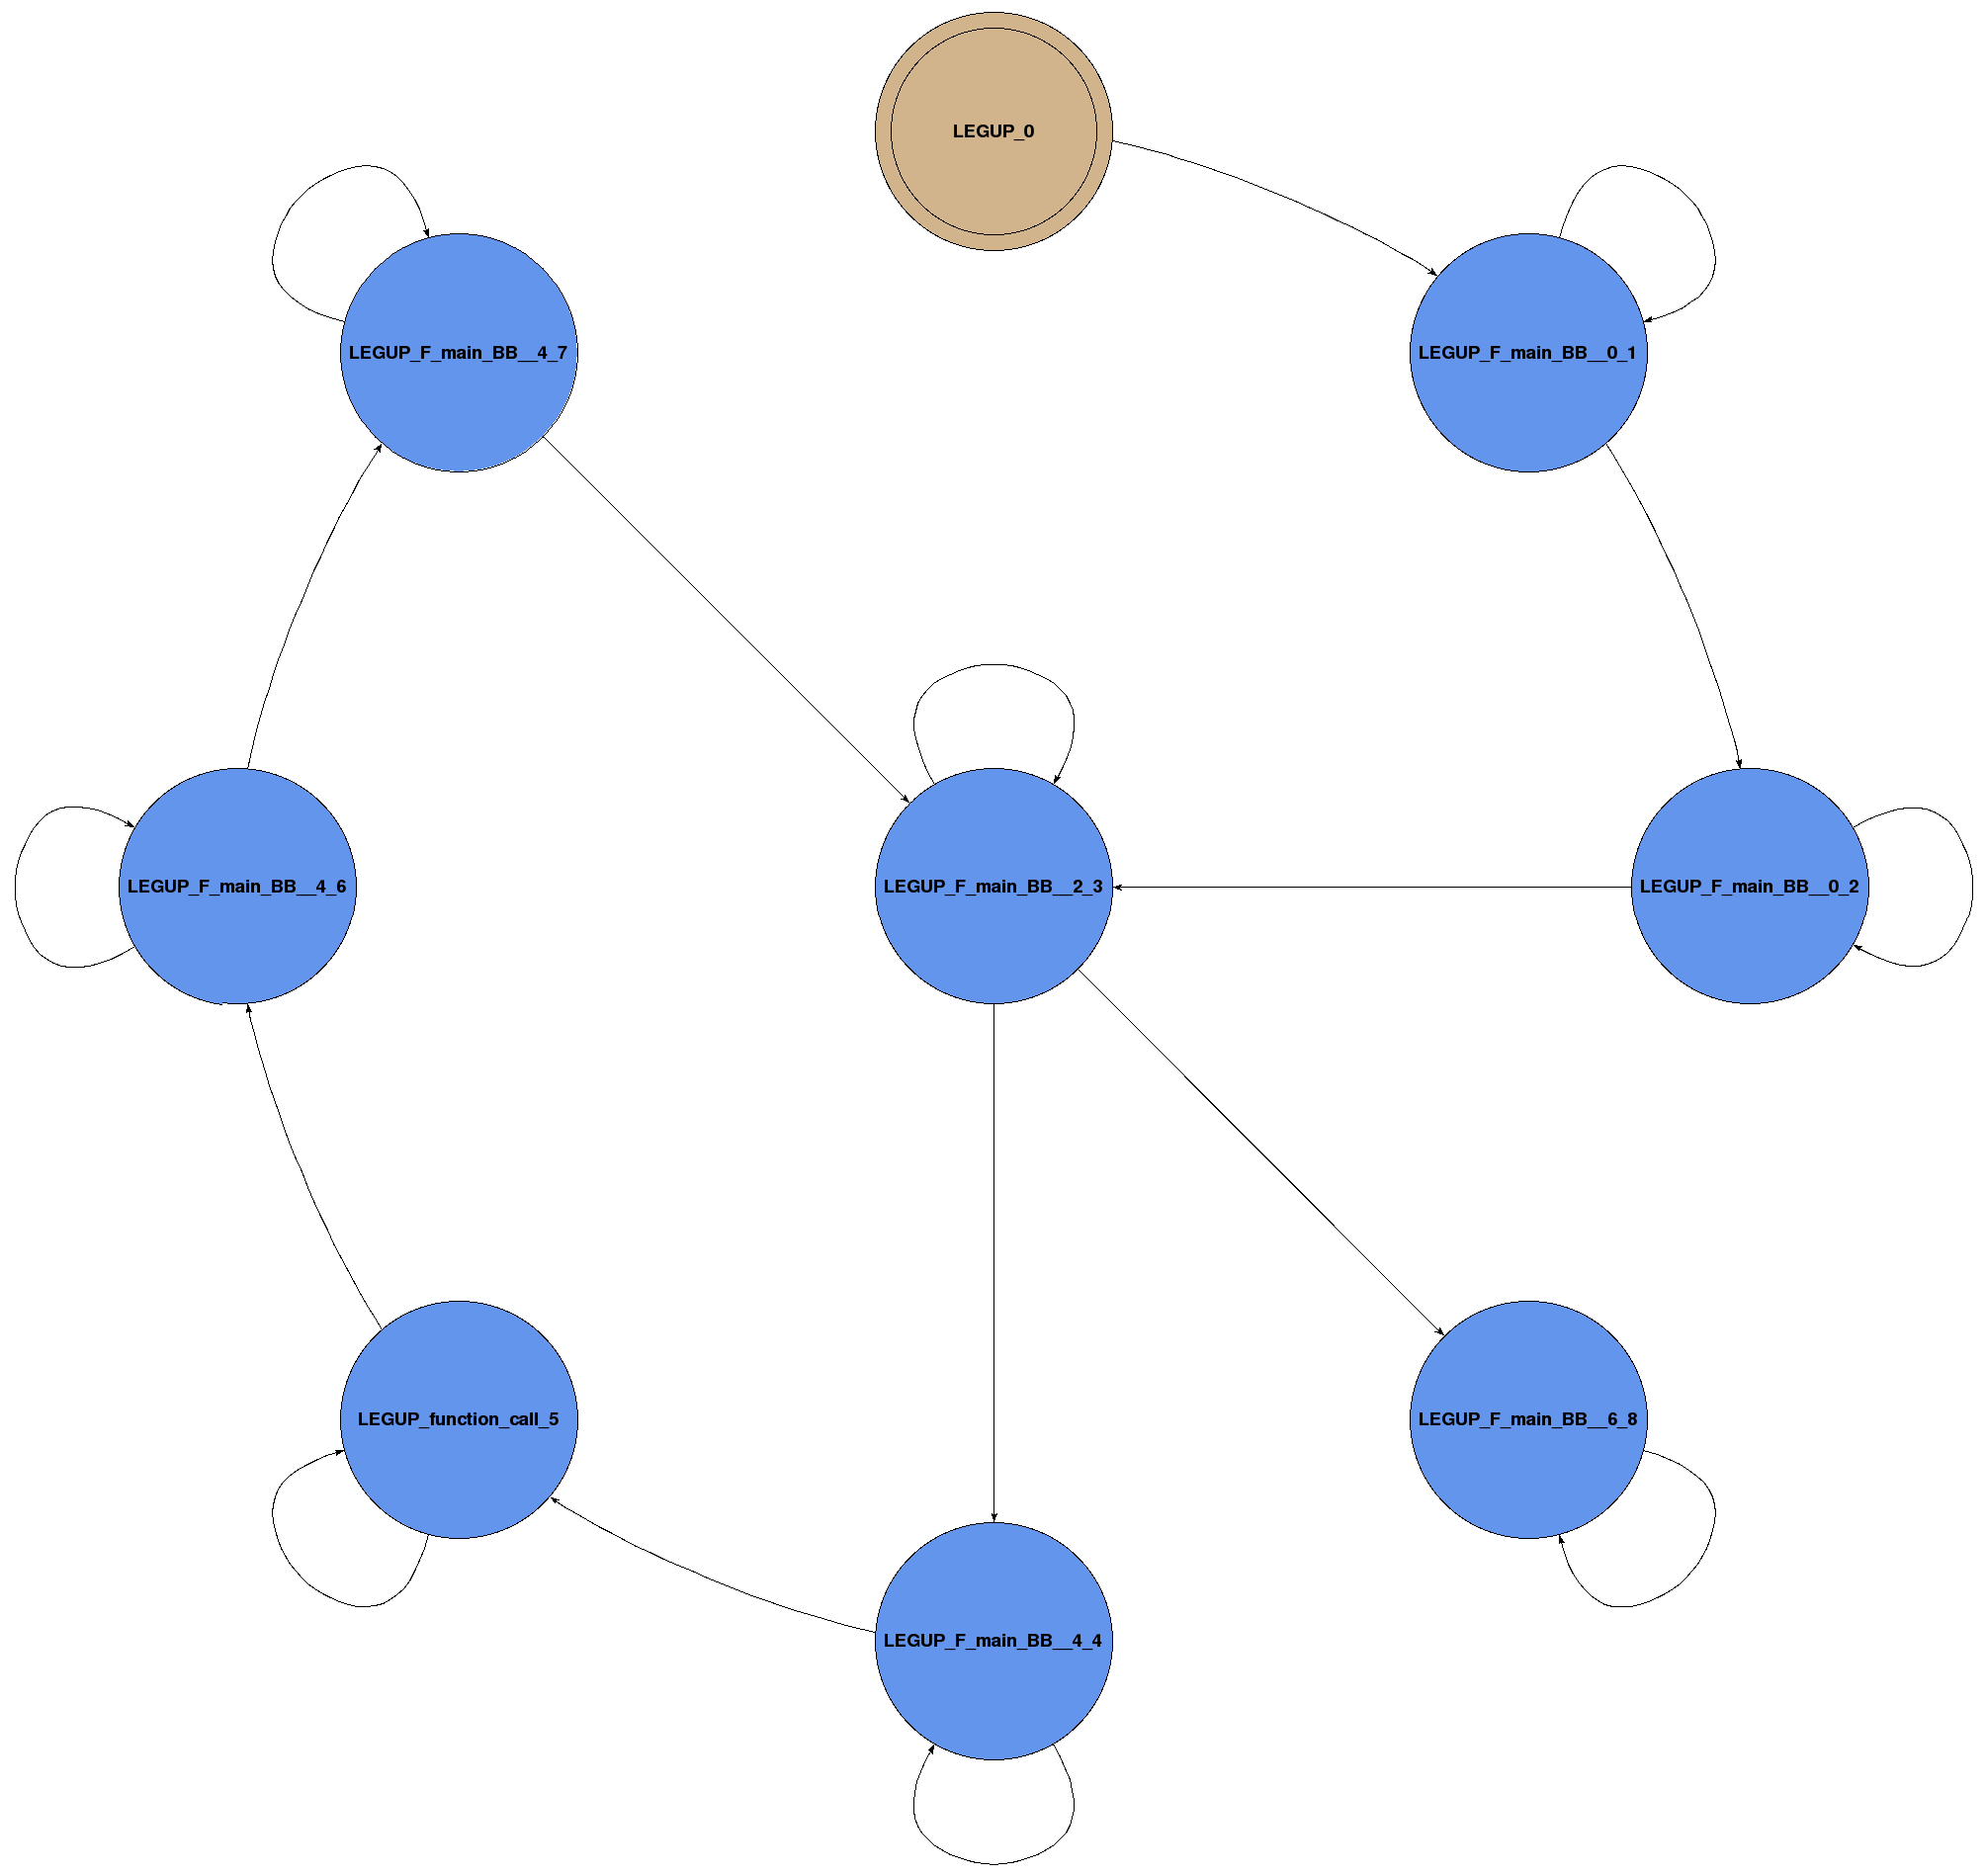
\includegraphics[width=0.9\textwidth]{../figs/VerilogFSM.png}
\caption{\label{fig:verilogfsm}State diagram of generated FSM}
\end{figure}
By looking at the state diagram, some parts from the C-code can be recognized. \textit{LEGUP\_0} is the initial state and the two following states is allocating and storing the volatile input parameter. \textit{LEGUP\_F\_main\_BB\_2\_3} is where the condition checking for the while loop is performed. The states below and left of the condition state is the states inside the while loop, and \textit{LEGUP\_F\_main\_BB\_6\_8} is the exit-state, signalizing the completion of the program.

Some signal assignments are shown in \cref{lst:verilogsignalassignment}. Each assignment is printed with the corresponding LLVM operation commented abowe, to increase readability of the code. The later assignment of output signals are not generated directly from an LLVM operation and does thus not have this operation printed along the assignment.
\begin{lstlisting}[caption={Verilog FSM},label=lst:verilogsignalassignment,float]
always @(*) begin
	/* main: %2*/
	/*   %3 = icmp eq i32 %done, 0*/
		main_2_3 = (arg_done == 32'd0);
end
always @(posedge clk) begin
	/* main: %4*/
	/*   %5 = call i32 @squared(i32 %inData) #1*/
	if ((cur_state == LEGUP_F_main_BB__4_4)) begin
		squared_arg_base <= arg_inData;
	end
end
always @(posedge clk) begin
	if ((cur_state == LEGUP_F_main_BB__4_6)) begin
		arg_outData <= main_4_5_reg;
	end
end
always @(posedge clk) begin
	if ((cur_state == LEGUP_F_main_BB__4_6)) begin
		arg_outData_valid <= 1'd1;
	end
	if (~((cur_state == LEGUP_F_main_BB__4_6))) begin
		arg_outData_valid <= 1'd0;
	end
end
always @(posedge clk) begin
	if ((cur_state == LEGUP_F_main_BB__4_7)) begin
		iterationFinish <= 1'd1;
	end
	if (~((cur_state == LEGUP_F_main_BB__4_7))) begin
		iterationFinish <= 1'd0;
	end
end
\end{lstlisting}

\subsection{Simulation}
\subsubsection{Simulation libraries}

LegUp generates local RAMs for each output-parameter to the main module, as these parameters needs to be declared as volatile. 

In the declaration of the modules ram\_dual\_port and rom\_dual\_port, a conversion function from an Altera library is used to convert .mif files to a format readable by Modelsim. The .mif-file contains initial content of memory. The code snippet that uses this library is shown in \cref{lst:alteralibrary}. If the design does not contain any initial memory values, this conversion method is not needed and could be removed from the design. As this is a feature in LegUp, this has not been altered at this time. This requires the library file to be included in the design filelist for simulation to be successful. The library-file is located in \textasciitilde/legup-4.0/ip/libs/altera/altera\_mf.v of the LegUp VirtualBox image. 
\lstset{language=Verilog, style=VerilogStyle}
\begin{lstlisting}[caption={Altera Library function used for memory management},label=lst:alteralibrary]
ALTERA_MF_MEMORY_INITIALIZATION mem ();
// modelsim can't read .mif files directly. So use Altera function to
// convert them to .ver files
mem.convert_to_ver_file(init_file, width_a, ram_ver_file);
$readmemh(ram_ver_file, ram);
\end{lstlisting}

In the physical implemented design, memory cannot be filled with initial values, and thus this section of code is not included in synthesis, indicated by the commented lines \verb!"synthesis_translate_off"! and \verb!"synthesis_translate_on"!. Also, since the library file is not synthesizable, it cannot be included in the filelist used for synthesis.

\subsubsection{Running simulation}
The generated Verilog code is simulated using QuestaSim. The simulation is executed by running the script \textit{RUN\_ALL} located in the rtl folder. The GUI of QuestaSim can be brought up by passing the argument \verb!-g! to the script, otherwise the simulation will be run in batch mode in the terminal.

To simulate the design, a suitable testbench needs to be provided. Fortunately, LegUp generates a testbench shell, meaning we only need to add the testcases we want to apply to the circuit. Since this is a simple example, we only provide a few testcases to ensure the design works as expected. 
\begin{lstlisting}[caption={Testcases for the example testbench},label=lst:tbcases]
initial begin
    arg_done <= 32'd0;
    arg_inData <= 32'd20;
    
    @(negedge reset);
    start <= 1;
    @(negedge clk);
    start <= 0;
    
    @(posedge iterationFinish);
    arg_inData <= 32'd100;
    
    @(posedge iterationFinish);
    arg_inData <= 32'd498;
    
    @(posedge iterationFinish);
    arg_done <= 32'd1;
end
\end{lstlisting}
\Cref{lst:tbcases} shows the testcases we apply to the circuit. Initial values of the inputs \textit{done} and \textit{inData} is set, and the testbench waits for a falling edge of the reset signal, set by the automatic generated testbench shell, before setting the \textit{start}-flag high for one clock cycle. At the two folloeing rising edges of the \textit{iterationFinished}-flag, a new value is assigned to the input \textit{inData}. At the third rising edge of the \textit{iterationFinished}-flag, the input \textit{done} is set to one, indicating the end of this run. A waveform from the simulation is shown in \cref{fig:simulationwave}. From the waveform we observe that the circuit has the expected behaviour. When the \textit{start}-flag is set, the FSM starts and the sub-module \textit{squared} starts to calculate the output value. When \textit{cur\_state} of the \textit{main}-module equals 7, the calculated value is assigned to the output \textit{outData}, and the \textit{valid}-flag for this output is set. The value on the output is correctly calculated for the given testcases. When \textit{cur\_state} equals 3, the {iterationFinish}-flag is set, as this is the state where the condition for the while loop is evaluated, i.e. one iteration of the loop is complete. Notice that the \textit{iteartionFinish}-flag is not set in the first occurrence of \textit{cur\_state} = 3, as this is the first encounter of the loop and not a finished iteration. When the input \textit{done} is set to 1 after the third \textit{iterationFinish}-flag, we observe that the loop terminates and the \textit{finish}-flag is set, indicating the end of the run.
\begin{figure}[hbpt]
\centering
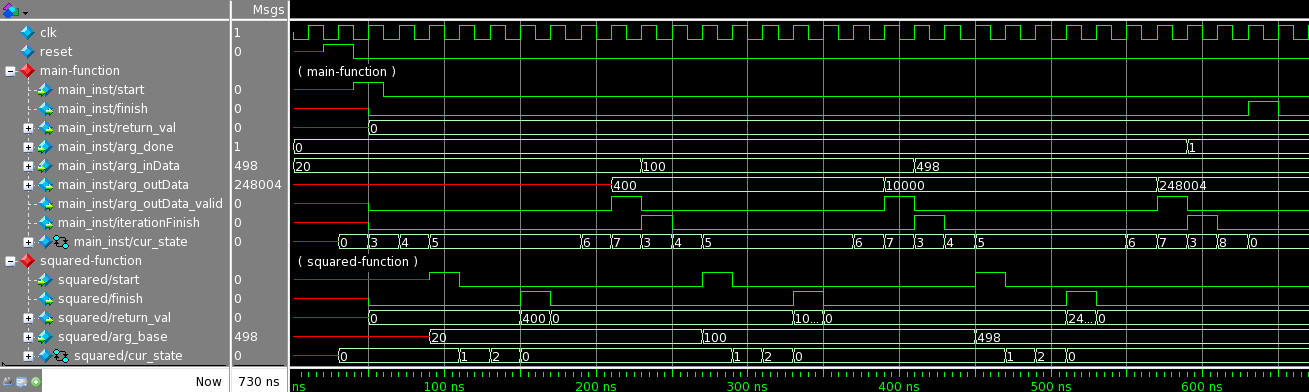
\includegraphics[width=0.99\textwidth]{../figs/SimulationWaveEX.png}
\caption{\label{fig:simulationwave}Simulation waveform of example design}
\end{figure}
\subsection{Synthesis}
The design is synthesized using a 180nm library. The area and frequency reports from the synthesis is presented in \cref{tab:synthreportex}.
\begin{table}[]
    \centering
    \begin{tabular}{lcr}
        \textbf{Parameter} && \textbf{Value} \\
        \toprule
        Number of ports && 137 \\
        Number of nets && 906 \\
        Number of cells && 505 \\
        Number of combinational cells && 371 \\
        Number of sequential cells && 133 \\
        Number of macros/black boxes && 0 \\
        Number of buf/inv && 135 \\
        Number of references && 31 \\
        \midrule
        Combinational area && 26740.929852 \\
        Buf/Inv area && 3466.108790 \\
        Noncombinational area && 20824.373009 \\
        Macro/Black Box area && 0.000000 \\
        Net Interconnect area && 39816.683686 \\
        \midrule
        Total cell area && 47565.302861 \\
        Total area && 87381.986547 \\
        \midrule
        Critical Path Length && 77.71 ns \\
        Maximum Frequency && 12.86 MHz\\
        \bottomrule
    \end{tabular}
    \caption{Caption}
    \label{tab:synthreportex}
\end{table}
To put the area of the synthesized design in perspective, the library defines a two-port NAND gate to be 9.9792 area units. The number of NAND2-equivalent gates for the design is then 8757 gates. This is a large amount for such a simple design, but the area overhead percentage of the design will shrink with larger designs. The reported \subsection{Layout}

\subsection{Power estimation}

\subsection{Constraint files}
LegUp uses constraint files to set constraints and settings for the \gls{hls}. The default values for necessary constraints is set in the default constraint-file located in \textasciitilde/legup4-0/example/legup.tcl. The default constraints can be overridden by adding a local constraint file. The filename of the local constraint file need to be specified in the Makefile for the constraints to take effect. This is done by adding the line \verb!LOCAL_CONFIG = -legup-config=config.tcl! to the Makefile, where config.tcl is the filename of the local constraint-file. 
\subsection{Makefile}
The minimal local Makefile of LegUp contains the following three lines:
\begin{verbatim}
  NAME=name
  LEVEL = ..
  include $(LEVEL)/Makefile.common
\end{verbatim}

The Variable \textit{NAME} is the name of the design. This variable will be used to name the output-files of the design. The Variable \textit{LEVEL} indicated the number of directory levels it is up to where the common Makefile is located. 1 level up is marked as .., 2 levels up is marked as ../.. and so on, just like in a standard Linux shell. Other parameters, like \textit{NO\_OPT} (disable optimization in the compilator) and \textit{NO\_INLINE} (avoid inlining functions in the program), can also be added to the Makefile for passing flags and settings to the compilation. In some cases, especially with simple test-programs, these two flags are necessary to prevent the compiler from optimize away the whole program.
\chapter{Resolving issues with LegUp}
The main focuses of this project has been to resolve the issues encountered in \cite{holm2015pro}, to make LegUp able to generate Verilog more suited for ASIC implementation and synthesis. This chapter will describe the process of resolving these issues and other alterations that has been made in order to ease the creation of a framework for architectural exploration of hardware.
\section{Approach}
In the future works section of the project, two different approaches to resolve the issues were proposed; post-processing and pre-processing. Both approaches have been explored, but the main section of solutions are based on the pre-processing alternative. The two following subsection will present the two approaches and give some reasoning to why one is chosen over the other.
\subsection{Post-processing}
With the post-processing approach, the idea is to alter the Verilog-code after it is generated, to make it more suitable for our needs. This approach is easy to work with, as we can concentrate on a single file, the output Verilog file. The drawback of this approach is that you only have the information available in the Verilog file at hand, making it hard to add functionality to the tool.

There exist multiple parser tools for Verilog, for instance Verilog-Perl from VeriPool, a Verilog parser library for Perl, and pyverilog, a Hardware Design Processing Toolkit for Python \cite{Takamaeda2015Pyverilog}. These tools can be used to parse the Verilog file, to build module, signal, and port hierarchy, and easily add, alter, or remove objects.
\subsection{Pre-processing}
The pre-processing approach involves changing the libraries in LegUp that performes the HLS operations, like allocation, scheduling, RTL-generation and Verilog printing. This requires deep knowledge of the libraries and its connections, to be able to find a good way to change the output. The large libraries is the main drawback of this approach. As LegUp is open-source, the possibilities of this approach are however endless, but getting the necessary knowledge of the libraries takes time.
\subsection{The chosen approach}
As it looked like the easiest solution, the post-processing alternative were explored first. However, it were soon realised that the things that could be done easily with this approach, also could be done quite easily with the pre-processing approach. Some larger issues, for instance assigning values to outputs, were not easily solvable by using the post-processing method. The focus were therefore directed towards the pre-processing alternative.

\section{TCL commands}
LegUp uses TCL commands for setting constraints and configure the HLS process. In order to not clutter the original implementation, and to provide additional functionality to LegUp, some new commands were created. New TCL-parameters can easily be added to LegUp by adding the parameter name to the array \textit{validParameters} and increasing the parameter \textit{NUM\_PARAMETERS} in the file \textit{LegupConfig.cpp}. The value of the parameter can then be read using the function call \verb!LEGUP\_CONFIG->getParameter("\%parameterName\%")! to get a string, or \verb!LEGUP\_CONFIG->getParameterInt("\%parameterName\%")! to get an integer. LegupConfig.h must be included to get access to LEGUP\_CONFIG. The most common use of TCL-parameters are to check if a parameter is set, and perform some action if it is, or to use the parameter to set a variable. An example could be a parameter that decides if a designated top-module shall be generated or not. The parameter is define by adding the below line to the constraint file:

\begin{verbatim}
set_parameter PRINT_TOP_MODULE 1
\end{verbatim}
The parameter can then be used to decide if the Top-module should be printer:
\lstset{language=C++,style=Cstyle}
\begin{lstlisting}
  if(LEGUP_CONFIG->getParameterInt("PRINT_TOP_MODULE") {
    printTop();
  } else {
    printVerilogWithoutTop();
  }
\end{lstlisting}

Another example is to use a parameter to set the name of the top-module. This can be used either for naming the top-module, or to select top-module in the simulation-settings. 
\begin{verbatim}
set_parameter TOP_MODULE_NAME "moduleName"
\end{verbatim}
\begin{lstlisting}
  std::string topModuleName = "top"; // Default name
  if(LEGUP_CONFIG->getParameter("TOP_MODULE_NAME") {
    topModuleName = LEGUP_CONFIG->getParameter("TOP_MODULE_NAME");
  }
\end{lstlisting}
In the second example, the getParameter() function will return false if the parameter is not set.

Other TCL-commands can also be defined by adding 
\begin{lstlisting}
  Tcl_CreateCommand(interp,
                    "set_custom_main_function",
                    set_custom_main_function,
                    legupConfig,
                    0);
\end{lstlisting}
Where the second parameter is the TCL-command and the third parameter is the handler function that will be called when the TCL-command is encountered.

\begin{description}
\item{\textbf{ASIC\_IMPLEMENTATION}} \hfill \\
This parameter is used to distinguish between the standard version of LegUp and the altered version that will be used in this thesis for generating modules suitable for ASIC implementation. If this parameter is set, all extra features described in the following subsections will be applied to the generated design. If the parameter is not set, the unaltered edition of LegUp will be used to generate the output.
\item{\textbf{set\_custom\_main\_function}} \hfill \\
This parameter can be used to define inputs and outputs in the main module, as described in \cref{subsubsec:inoutparameter}. The  
\item{\textbf{ENCLOSING\_WHILE\_LOOP}} \hfill \\
Main-function has enclosing while loop (for streaming inputs/outputs). Will generate \textit{iterationFinish}-signal when iteration of while loop is finished,
\item{\textbf{SEPARATE\_TB\_FILE}} \hfill \\
Parameter decides if testbench is printed in same or a separate file. The filename of the separate testbench-file will be test\_main.v, according to Nordic's naming standard, but this can easily be changed or made dynamic by setting the constraint \textit{set\_custom\_testbench\_filename}.
\item{\textbf{SEPARATE\_TB\_FILENAME}} \hfill \\
Takes testbench filename as parameter and outputs testbench to a file with this name. Will not work if \textit{SEPARATE\_TB\_FILE} is not set. Default is \textit{test\_main.v}
\item{\textbf{TB\_TESTCASE\_FILE}} \hfill \\
As described in \cref{subsec:tbgen}, a way to automatically include testcases into the testbench is implemented. This parameter provides the filename of a file containg testcases for the testbench. If the parameter is not set, no testcases will be added to the testbench.
\item{\textbf{REMOVE\_UNUSED\_LOCAL\_RAMS}} \hfill \\
By declaring input parameters as volatile, a local RAM will be generated in the main module for each output signal we create. These RAMs is not used for anything useful and can therefore be removed to save area. If set, Local RAMs in main are removed \textit{if} the value stored to the RAM is assigned to an output instead.
\end{description}




\section{Removing memory controller}
One of the main issues with using LegUp for 

\section{\label{subsec:inoutdecl}Declaring inputs and outputs}
Each function declared in a C program will be translated into a Verilog-module by LegUp. Since LegUp primarily is designed for implementing hardware accelerators for FPGAs, it does not handle inputs and outputs well to and from the top module. In an ASIC implementation, inputs and outputs are essential to most module design and must therefore be easy to implement. In a C-program written for execution on a computer the input parameters to the main function is defined to be on the form "int main(int argc, char *argv[])". This limits the possibility to declare inputs to the module with any data-type. To solve this problem, the flag \textit{-ffreestanding} has to be passed to the clang compiler frontend of LLVM. The compiler will then consider the C-code to contain a freestanding - not a hosted - environment, and therefore not care about what types of inputs and return values the \textit{main}-function has. In LegUp, the flag can be passed to the compiler by adding it to the variable \textit{CLANG\_FLAG} in the file \textit{Makefile.config}.

The solution that would have been used in a hosted environment is to use pointers as input and output values as pass-by-reference.

Two different solutions for declaring inputs and outputs are considered and implemented. Both solutions are based on declaring both inputs and outputs as parameters to the main function.
\subsection{Name prefix}
The first solution is to use a prefix to distinguish between input and output parameters. To use a prefix that is seldom used in a variable name, the prefix is set to \textit{\_\_out\_}. Previously, LegUp assumed all function parameters were inputs, and added the signals to the RTLModule. This has been altered to check the name of the parameter and add it as an output reg if the name starts with \textit{\_\_out\_} or otherwise, add it as an input.

\begin{lstlisting}
std::string sigName = i->getName();
if (sigName.find("__out_") == 0) {
  sigName = sigName.substr(6, std::string::npos);
  i->setName(sigName);
  rtl->addOutReg(verilogName(i), RTLWidth(i->getType()));
  string validSigName = "arg_" + sigName + "_valid";
  rtl->addOutReg(validSigName);
} else {
  rtl->addIn(verilogName(i), RTLWidth(i->getType())); 
}
\end{lstlisting}
The advantage of this method is that it is easy to implement and easy to use, as the user only has to remember the name prefix when writing the functional specification. The name-prefix can also be useful in other sections of the program, as we will see later in section \ref{sec:assValueToOutput}. The disadvantage is that the name prefix needs to be used throughout the program. It would however be preferable to use a temporary variable in the program until the final value is calculated and ready to be assigned to the output. This will reduce the amount of times the name-prefix must be used.
The name prefix will be stripped by LegUp, making the signal in the final Verilog-module look much cleaner.
\subsection{\label{subsubsec:inoutparameter}TCL-command}
The other alternative is to declare in a TCL-command if each parameter is input or output. This also makes it possible to declare the size of the signal, but LegUp does not allow setting the size of the signals to a size lower than the size of what will be assigned to the signal.

The TCL-command \textit{set\_custom\_main\_function} described above, creates a vector with objects of the class CustomVerilogIO, each containing one input or output signal to the main module. The parameters can then be added as input or output to the RTLModule based on this information.
\begin{lstlisting}
std::vector<CustomVerilogIO> cmIO = LEGUP_CONFIG->getCustomMainIO();
for (std::vector<CustomVerilogIO>::iterator it = cmIO.begin();
     it != cmIO.end(); ++it) {

  CustomVerilogIO &cmIO = *it;

  if (cmIO.isInput && (cmIO.name == i->getName().str())) {
    rtl->addIn(verilogName(i),
               RTLWidth(cmIO.bitFrom, cmIO.bitTo));
  } else if (cmIO.name == i->getName().str()) {
    rtl->addOutReg(verilogName(i),
                   RTLWidth(cmIO.bitFrom, cmIO.bitTo));
  }
}
\end{lstlisting}

\section{\label{sec:assValueToOutput}Assigning values to outputs}
In \cref{subsec:inoutdecl} two methods of declaring parameters as outputs in the generated module were presented. Unfortunately, assigning values to a input parameter is undefined behaviour in C. This means that even though the compiler will generate LLVM IR that perform this operations, they are not handled in the LegUp backend pass that transforms the IR into Verilog. The result is that a signal declared as output is assigned to a local RAM module and no assignments to the output exists.

To overcome this issue, the idea to look at the LLVM IR code to see if any information about assignment could be gathered here and used in LegUp to assign the correct values to the output were brought up. 
\lstset{language=C,style=Cstyle}
\begin{lstlisting}[caption={Simple C-code example for LLVM IR parsing},label=lst:cllvmirparsercode]
void main(int inDataA, int inDataB, volatile int __out_outData) {
    while (1) {
        __out_outData = inDataA * inDataB;
    }
    return;
}
\end{lstlisting}
\lstset{language=LLVM,style=LLVMStyle}
\begin{lstlisting}[caption={LLVM IR code for simple parsing example},label=lst:llvmirparsercode]
define void @main(i32 %inDataA, i32 %inDataB, i32 %__out_outData) #0 {
  %1 = alloca i32, align 4
  store volatile i32 %__out_outData, i32* %1, align 4
  br label %2

; <label>:2                                       ; preds = %2, %0
  %3 = mul nsw i32 %inDataA, %inDataB
  store volatile i32 %3, i32* %1, align 4
  br label %2
                                                  ; No predecessors!
  ret void
}
\end{lstlisting}
Lets analyze the LLVM IR code output from compilation, shown in \cref{lst:llvmirparsercode}. On line 2 the temporary register \%1 is created. On line 3, the input parameter declared as volatile, \textit{\_\_out\_outData}, is stored to this register. On line 7, the multiplication calculation of the inputs inDataA and inDataB is stored to a new temporary register \%3. On line 8, the content of register \%3 is stored back to register \%1. This information can be exploited to create a program that traces stores, back to the original input parameter. In this example, we can easily see that the multiplication calculation easily can be traced back to the output \textit{\_\_out\_outData}, but in more complex programs, this tracing might not be that easily done. The solution would be to create a script that parses through the IR code and makes these connections for us. 

When LegUp generates signals, they will be named by the convention \%functionName\%\_\%labelNumber\%\_registerNumber\%. This means that the example above will create the signals (or RAM modules for parameters and arrays) \textit{main\_0\_1} from line 2 and \textit{main\_2\_3} from line 7.
\subsection{LLVM IR assignment parser program}
A program were created to parse the LLVM IR generated by the compilation. This section will explain in words and pseudo-code how the program works. The full source code of the parser program is included in \ref{lst:llvmirparserprogramcode} in the appendix. The program takes two command-line arguments when called, name of the input file and name of the output file. The input file should be the final LLVM IR file generated by LegUp, named \textit{\%designName\%.ll}. The output can be what you like, but the default file-name used in LegUp for reading of the output is \textit{LLVMParsed.log}. The program consist of two parts, the first part handles the reading and parsing of the input file, the second part is handling the generating of the output file. The program is created to only care about the main-function, as this is the module where it is vital to have multiple output signals. The program can easily be changed by altering the source code, if found necessary at a later point.

A pesudo-code describing the first part of the program is shown in \cref{alg:llvmparserpart1}. The parser starts by looking for the main-function. When in the main-function, the program looks for lines containing stores or labels. If a store is found, the source and target register of the store is stored in a vector, together with the current label. If a new label is found, the label is set as the current label.

\algnewcommand\algorithmicto{\textbf{to}}
\algnewcommand\algorithmicand{\textbf{and}}
\begin{algorithm}
  \caption{Pseudo-code of input file handling in LLVM IR parser program
  \label{alg:llvmparserpart1}}
  \begin{algorithmic}[1]
    \Require{inFile and outFile should be passed as arguments}
    \Statex
    \If{$inFile.open()$}
    \State $currentLabel \leftarrow 0$
    \State $inMain \leftarrow false$
      \While{$inFile.getNextLine() \neq inFile.end()$}
        \If{$inMain$}
          \If{$lineStartWith() = "~~store"$}
            \State $newSource \leftarrow sourceRegisterFromLine$
            \State $newTarget \leftarrow targetRegisterFromLine$
            \State $sources.insert(newSource)$
            \State $targets.insert(newTarget)$
            \State $labels.insert(currentLabel)$
          \ElsIf{$lineStartWith() = ";~<label>:"$}
            \State $currentLabel \leftarrow labelNumberFromLine$
          \ElsIf{$lineStartWith() = "\}"$}
            \State $inMain \leftarrow false$
          \EndIf
        \ElsIf{$lineStartWith() = "define~\%type\%~@main"$}
          \State $inMain \leftarrow true$
        \EndIf
      \EndWhile
    \EndIf
  \end{algorithmic}
\end{algorithm}
A pesudo-code describing the second part of the program is shown in \cref{alg:llvmparserpart2}. A double for-loop is needed to check each target against each other target. The C-example above will store the values shown in \cref{tab:llvmirparservectors} in the vectors. 
\begin{table}[hbtp]
    \centering
    \begin{tabular}{ccc}
    \textbf{sources} & \textbf{targets} & \textbf{labels} \\
    \toprule
      \_\_out\_outData & 1 & 0 \\
      3 & 1 & 2 \\
    \bottomrule
    \end{tabular}
    \caption{Caption}
    \label{tab:llvmirparservectors}
\end{table}
By comparing the first target against the second target in the table, it can easily be seen that the second source is stored to the same target as the first source. The output format is given by:
\verb!"sources[i] sources[j] labels[j] labels[i] targets[i]"!
The output from the above example will then be:
\verb!"outData 3 2 0 1"!.
This implies that the signal \textit{main\_2\_3} should be assigned to the output \textit{outData}. The two last values, 0 and 1, are included as they will be used in a trick in \cref{subsec:assigningoutputsignals} to simplify the process of assigning signals to output ports.
\begin{algorithm}
  \caption{Pseudo-code of output file handling in LLVM IR parser program
  \label{alg:llvmparserpart2}}
  \begin{algorithmic}[1]
    \If{$outFile.open()$}
    \State $done \leftarrow \{\}$
      \For{$i \leftarrow 0~\algorithmicto~targets.size()$}
        \For{$j \leftarrow 0~\algorithmicto~targets.size()$}
          \If{$targets[i] = targets[j]~\algorithmicand~i \neq j~\algorithmicand~sources[i] \notin done$}
            \State $newSource \leftarrow sourceRegisterFromLine$
            \State $newTarget \leftarrow targetRegisterFromLine$
            \State $done.insert(sources[j])$
            \If{$sources[i].lineStartWith() = "\_\_out\_"$}
              \State $parameterName \leftarrow sources[i].strip(\_\_out\_)$
              \State $outFile.print(parameterName)$
              \State $outFile.print(sources[j])$
              \State $outFile.print(labels[j])$
              \State $outFile.print(labels[i])$
              \State $outFile.print(targets[i])$
              \State $outFile.print("\backslash n")$ \Comment{$Newline$}
            \EndIf
          \EndIf
        \EndFor
      \EndFor
    \EndIf
  \end{algorithmic}
\end{algorithm}
Execution of the program is added to the common Makefile, \textit{Makefile.common}, just before running the LegUp backend pass that generated Verilog output. The program is called by the line:
\begin{verbatim}
$(LEVEL)/LlvmParser.run $(NAME).ll LlvmParsed.log
\end{verbatim}

\subsection{\label{subsec:assigningoutputsignals}Assigning output signals}
As described in \cref{sec:legupclasses}, any RTLSignal that exist in an RTLModule can be found by calling the function \textit{find()}, with the name of the signal passed as a string parameter. A RTLSignal can have multiple drivers and conditions, and the i-th driver or condition can be found by calling getDriver(i) and getCondition(i). The initial idea when the LLVM IR parser program was created, was to find each of the signal and connect it to the correct output.

For every parameter to the function, the compiler will allocate a register and store the parameter value to this register. Whenever a store to a parameter is performed, this value will be stored to the first allocated register. In LegUp, the allocated register will be implemented as a RAM module and all stores to the parameter will be stored to this ram. This information can be exploited to easily assign values stored to this RAM to the output port instead.

\begin{figure}
        \centering
        \begin{subfigure}{0.49\textwidth}\centering%no!\hfill
                    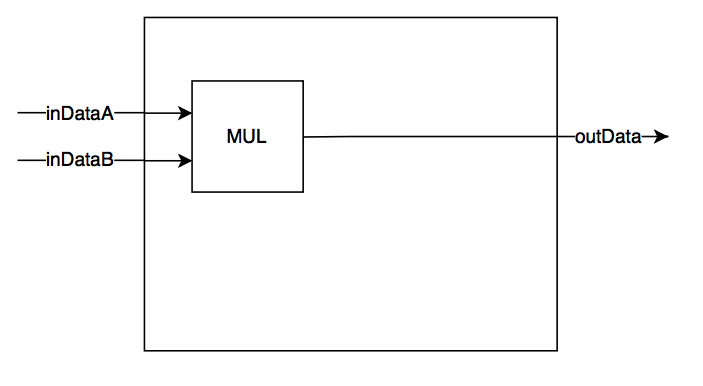
\includegraphics[width=\linewidth]{figs/OutputAssignment1.png}
                \caption{What we want to achieve}
  \label{fig:assignoutputs1}
       \end{subfigure}%
%no, don't use ~!           ~ %add desired spacing between images, e. g. ~, \quad, \qquad etc.
      %(or a blank line to force the subfigure onto a new line)
    \hfill
        \begin{subfigure}{0.49\textwidth}\centering
                    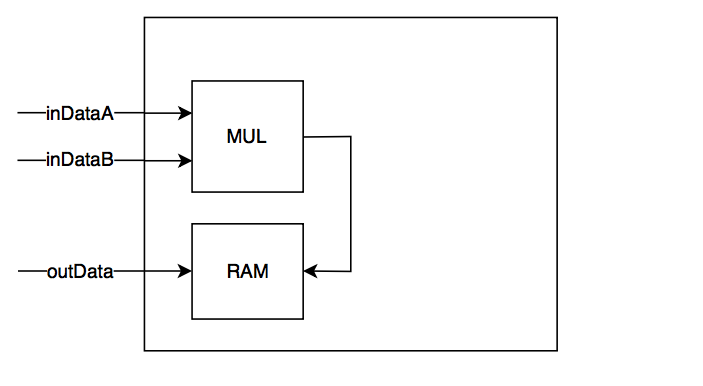
\includegraphics[width=\linewidth]{figs/OutputAssignment2.png}
                \caption{What the compiler/Legup thinks we want to achieve}
  \label{fig:assignoutputs2}
       \end{subfigure}%
    \hfill
        \begin{subfigure}{0.49\textwidth}\centering
                    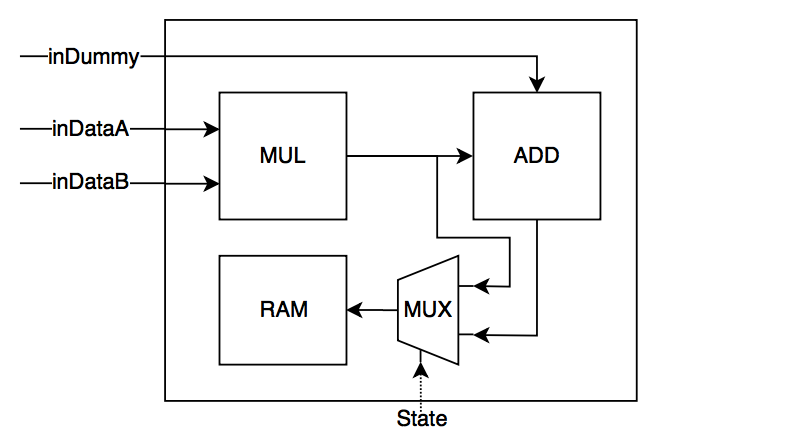
\includegraphics[width=\linewidth]{figs/OutputAssignment3.png}
                \caption{An example with multiple stores to \textit{outData}}
  \label{fig:assignoutputs3}
       \end{subfigure}%
    \hfill
        \begin{subfigure}{0.49\textwidth}\centering
                    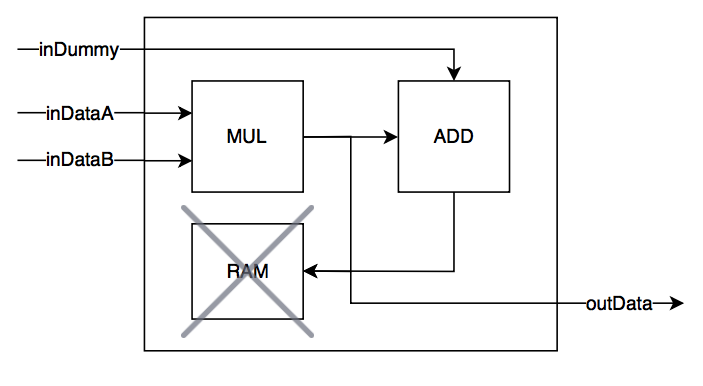
\includegraphics[width=\linewidth]{figs/OutputAssignment4.png}
                \caption{The solution}
  \label{fig:assignoutputs4}
       \end{subfigure}%

\caption{4 figures}
\label{fig:assigningoutputs}
 \end{figure}
\cref{fig:assigningoutputs} tries to illustrate the problem with assigning outputs. In \cref{fig:assignoutputs1}, the module we would expect from the C-code in \cref{} is shown. The two inputs are multiplied together and output to outData. In reality, what happens in the generated Verilog is shown in \cref{fig:assignoutputs2} and in \cref{fig:assignoutputs3}, when extended with an extra ADD module that stores to \textit{outData}. Instead of assigning the calculated values to the output, they are stored in a RAM module. The solution to this problem is shown in \cref{fig:assignoutputs4}. By "hijacking" the input signal to the RAM module and assigning it to the output, \textit{outData}, we get the expected functionality. 

The RAM module will be named by the same convention as signals, naming the RAM in this module \textit{main\_0\_1}. The dataIn signal of the RAM module is named \%ramName\%\_in\_a. This is the signal we want to "hijack". The "hijacking" is performed as described in \cref{alg:assignoutputsignals}. The name of the output ports are read from the file output from the LLVM IR parser program, together with the name of the corresponding RAM modules. For every output port, each driver-condition pair stored to the RAM module is added as a conditional driver to the output port.
\makeatletter
\let\OldStatex\Statex
\renewcommand{\Statex}[1][3]{%
  \setlength\@tempdima{\algorithmicindent}%
  \OldStatex\hskip\dimexpr#1\@tempdima\relax}
\makeatother
\begin{algorithm}
  \caption{Pseudo-code of assigning values to outputs
  \label{alg:assignoutputsignals}}
  \begin{algorithmic}[1]
    \For{$i \leftarrow 0~\algorithmicto~outputPorts.size()$}
      \State $outputPort \gets find(output~signal~name)$
      \State $ramSignal \gets find(RAM~module~inData~signal)$
      \For{$j \gets 0~\algorithmicto~ramSignal.getNumDrivers()$}
        \State $outputPort.addCondition(ramSignal.getDriver(j),$
        \Statex[9] $~~~~ramSignal.getCondition(j))$
      \EndFor
    \EndFor
  \end{algorithmic}
\end{algorithm}

\subsection{Removing local RAMs}
After reassigning the RAM stores to the output port, the generated RAM module corresponding to the input parameters are no longer needed. The ram modules can be removed to save area and power consumption. To make this operation optional, the TCL-parameter \textit{REMOVE\_UNUSED\_LOCAL\_RAMS} were added. By setting this parameter, the local RAM modules will be removed. All RAMs local to a module is stored together with its corresponding function (from the C-code) in a variable, \textit{	isLocalFunctionRam}. When the RAM is removed, it is simply removed from this variable. In addition to removing the RAM module, all signals to and from the RAM needs to be removed as well. Notice that only the RAMs generated by output parameters are removed from the main module. RAM modules can also be generated by arrays and other large data structures, but these will not be removed in any cases.

\section{Streaming inputs/outputs}
For most module designs to be useful, fast and , it must be able to continuously take new inputs and generate outputs, without having to start and stop the entire module each time, with all the overhead in time this would require. The way LegUp is designed, functions are used as hardware accelerators, meaning it gets some input, performs some calculations and the outputs the result. The module is then finished and will not run again until next time the accelerated function is called. For this approach to work for an ASIC implementation, a top module would need to be created to assign new inputs and start the module again once it is finished with the last iteration. This would create a lot of unwanted overhead, both in size and speed. A better solution would therefore be to add a while loop inside the main function of the C program to make the program run continuously.

With this solution some new issues arise. 
First we need a way to stop the module if all calculations are finished. This can easily be handled by adding a input parameter to the main function in the C-program, lets call it done, which is used as condition for running the while-loop. This parameter will then correspond to a signal in the Verilog-module that can be used to terminate the module. No alterations to LegUp is performed to resolve this issue, as it can be resolved manually by the user. This signal could not be added by LegUp, as it would require major alterations to the generated data-flow.

Secondly, we need a way to know when an output has valid data. A simple solution here is to generate a valid-flag for each output signal. These flags are created simultaneously with the outputs being connected to the driving signals, as described in \ref{sec:assValueToOutput}. The signals shall be valid only in the first clock cycle after the output signal has changed. To achieve this, two condition signals has to be created, one when the output is valid, and one when the output is not valid. The valid condition shall be set in any state where the output signal is assigned, i.e. the conditions gathered from the RAM module \textit{dataIn}-signal, and not valid in all other states. To create the valid-signal is straightforward, by adding the conditions from the RAM signal. To create the not valid signal are a bit more tricky. By creating an RTLOp-signal, AND-ing together all the valid states, and creating a second RTLOp-signal NOT-ing the first RTLOp signal, we will have the desired signals. The tricky part arises from the AND operation only being able to take two operands, making it hard to create code handling special cases of few and odd number of valid states. The source code of how this is handled is included in \cref{sec:validsinglssourcecode}.

The third and final issue we need to handle is that we need a way t know when an iteration of the loop is finished. This \textit{iterationFinish}-flag should be set in the state preceding the final state of the FSM.
\lstset{language=C,style=Cstyle}
\definecolor{LightGray}{gray}{0.9}
\begin{listing}[ht]
\begin{minted}
[
breaklines,
%frame=lines,
frame=single,
%framesep=2mm,
baselinestretch=1.2,
bgcolor=LightGray,
fontsize=\footnotesize,
linenos,
tabsize=2,
]
{cpp}
RTLSignal *interationFinish = rtl->addOutReg("interationFinish");

connectSignalToDriverInState(interationFinish, ONE, (--fsm->end())->getPrevNode());
interationFinish->addCondition(rtl->addOp(RTLOp::Not)->setOperands(interationFinish ->getCondition(0)), ZERO);
\end{minted}
\caption{Example with line numbers enabled}
\end{listing}
\begin{lstlisting}
RTLSignal *interationFinish = rtl->addOutReg("interationFinish");

connectSignalToDriverInState(interationFinish, ONE, (--fsm->end())->getPrevNode());
interationFinish->addCondition(rtl->addOp(RTLOp::Not)->setOperands(interationFinish->getCondition(0)), ZERO);
\end{lstlisting}
\begin{lstlisting}[caption={FIR-filter implemented in C},label=lst:firfilterc]
void main( int done ) {
  // Variable setup etc. can be done here.
  while(done == 0) {
    // Module operations are performed here
  }
  // No operations can be done here.
  return;
}
\end{lstlisting}

\section{\label{subsec:tbgen}Testbench generation}
LegUp did generate a basic testbench shell, but this were very static and incorporated into the same file as the module design, making it impractical to use in Nordic's toolflow. The generated testbench consisted of a testbench module, main\_tb, which instantiate the top module, \textit{top}, and sets reset, start and waitrequest flags. The input and output signals in the top module does not contain custom signals from the main module, and in an ASIC implementation we are not interested in the memory controller and additional modules declared/instantiated in the top module. The solution then, became to instantiate the main module instead and add each input or output by iterating over the ports in the main module.

\begin{lstlisting}
RTLModule *t = m->addModule("main", "main_inst");
if (LEGUP_CONFIG->getParameterInt("ASIC_IMPLEMENTATION")) {
  RTLModule *rtl = alloc->getModuleForFunction(alloc->getModule()->getFunction("main"));
  if (rtl->getName().compare("main") == 0) {
    for (RTLModule::const_signal_iterator i = rtl->port_begin(), e = rtl->port_end(); i != e; ++i) {
      const RTLSignal *s = *i;
      RTLSignal *d;
      string type = s->getType();
      if (!type.empty()) {
        if (type.compare(0, 6, "output") == 0) {
          d = m->addWire(s->getName(), s->getWidth());
          t->addOut(s->getName(), s->getWidth())->connect(d);
        } else {
          d = m->addReg(s->getName(), s->getWidth());
          t->addIn(s->getName(), s->getWidth())->connect(d);
        }
      }
    }
  }
}
\end{lstlisting}

As the testbench does not come with any form of testcases or applied signals, the testbench generater is extended to input Verilog code from a file specified by the TCL-parameter \textit{TB\_TESTCASE\_FILE}. This allows the user to specify testcases in this file, and it will automatically be inserted into the testbench file inside the testbench module. The code will be placed inside the module, but not inside any procedural blocks. This allows the user to add the preferred procedural block in the specified testcase file. An example testcase file can then be:

\lstset{language=Verilog, style=Verilogstyle}
\begin{lstlisting}
always @(iterationFinish) begin
  if (iterationFinish == 1) begin
    $display("At t=%t, Loop iteration finished", $time);
  end
end
\end{lstlisting}
or
\begin{lstlisting}
initial begin
    inData <= 100;
    @(posedge clk)
    inData <= 0;
    @(posedge clk);
    $display("At t=%t, outData=%d", $time, outData);
end
\end{lstlisting}
This automatic insertion of testcases, enables the script to first run HLS and then run simulation on the generated design and testbench.

\section{Coding constraints}
Due to some alterations made to the LegUp libraries, some additional constraints need to be followed when writing the functional specification to ensure correct output. The following subsections will describe these constraints.
\subsection{Structs}
To support structs, byte-enable must be supported by the RAM or ROM module used to store the data. The RAM and ROM modules inferred by LegUp does not support byte-enable, resulting in struct support not being present when writing the functional specification. If structs are used in the code, LegUp will use an altsyncram-module instead of inferring RAMs. The altsyncram-module is not supported by the IC-compiler toolflow used at Nordic for synthesis, and inferred RAM-modules must therefore be used. 
\subsection{Pointers}
Pointers are used to reference an object in memory, opposed to passing a copy of the actual object between function. This reduces both CPU-time and memory-space, as objects does not need to be copied every time it is used, and makes it possible to alter a memory object directly without implicit load and store operations. As the memory controller used to pass data between different modules are unwanted in an ASIC implementation, support for pointers are limited to use inside the function where the pointer is declared. This limitation is a big drawback with the additions to LegUp.

\chapter{\label{chp:createframework}Creating the framework}
\section{Create new project}
To create a new project, the directory hierarchy needs to be copied from a source to the destination, and directories and filenames need to be altered to match the design name. Filelist and setting files also needs to be altered to include the correct design file names. This process is automated into a bash script, \textit{CreateNewProject.sh}. To run the script, the directory \textit{\_source}, containing the source project, must be present in the directory where the script is run.

The directory- and file-tree of the framework is shown in \cref{fig:frameworkdirtree}. Directories are colored cyan, executables and scripts are colored teal, and other design and constraint files are colored violet. File comment or description are in black. Each file is described in the comment on the right side. 
\begin{figure}
\centering

\begin{minipage}{0.99\textwidth}
    \renewcommand*\DTstyle{\sffamily\tiny}
    \dirtree{%
    .1 \textcolor{cyan}{\slash}.
    .2 \textcolor{cyan}{\_source}.
    .3 \textcolor{cyan}{ip}.
    .4 \textcolor{cyan}{designname}.
    .5 \textcolor{cyan}{hls}.
    .6 \textcolor{teal}{constraintsGenerator{.}run} \dotfill \:\:\begin{minipage}[t]{5.4cm}
                                                    Program to generate constraint and Makefiles
                                                    \end{minipage}.
    .6 \textcolor{violet}{constraints{.}xlsx} \dotfill \:\:\begin{minipage}[t]{5.4cm}
                                                            Setup-file for constraint-generator
                                                            \end{minipage}. 
    .5 \textcolor{cyan}{lay}.
    .6 \textcolor{teal}{Makefile} \dotfill \:\:\begin{minipage}[t]{5.4cm}
                                                    Makefile for running layout
                                                    \end{minipage}.
    .5 \textcolor{cyan}{pow}.
    .6 \textcolor{teal}{Makefile} \dotfill \:\:\begin{minipage}[t]{5.4cm}
                                                    Makefile for running power analysis
                                                    \end{minipage}.
    .6 \textcolor{teal}{power\_analysis{.}tcl} \dotfill \:\:\begin{minipage}[t]{5.4cm}
                                                    Settings file for power analysis
                                                    \end{minipage}.
    .5 \textcolor{cyan}{rtl}.
    .6 \textcolor{violet}{designname{.}fl} \dotfill \:\:\begin{minipage}[t]{5.4cm}
                                                    Filelist specifying files in the design
                                                    \end{minipage}.
    .6 \textcolor{violet}{designname{.}v} \dotfill \:\:\begin{minipage}[t]{5.4cm}
                                                    Verilog designfile generated by LegUp
                                                    \end{minipage}.
    .5 \textcolor{cyan}{sim}.
    .6 \textcolor{cyan}{run}.
    .7 \textcolor{violet}{designname{.}args} \dotfill \:\:\begin{minipage}[t]{5.4cm}
                                                            Argument simulation tool
                                                            \end{minipage}.
    .7 \textcolor{violet}{designname{.}comp} \dotfill \:\:\begin{minipage}[t]{5.4cm}
                                                            Compilation parameter file for simulation{.} Specifies filelist for design and testbench{.}
                                                            \end{minipage}.
    .7 \textcolor{violet}{designname{.}sim} \dotfill \:\:\begin{minipage}[t]{5.4cm}
                                                            Simulation parameter file for simulation{.} Specifies top-level testbench module and simulation options{.}
                                                            \end{minipage}.
    .7 \textcolor{violet}{modelsim{.}ini} \dotfill \:\:\begin{minipage}[t]{5.4cm}
                                                            Settings-file for simulation tool
                                                            \end{minipage}.
    .7 \textcolor{teal}{RUN\_ALL} \dotfill \:\:\begin{minipage}[t]{5.4cm}
                                                            Script to run simulation
                                                            \end{minipage}.
    .6 \textcolor{cyan}{tb}.
    .7 \textcolor{violet}{test\_designname{.}fl} \dotfill \:\:\begin{minipage}[t]{5.4cm}
                                                    Filelist specifying files in testbench
                                                    \end{minipage}.
    .7 \textcolor{violet}{test\_designname{.}v} \dotfill \:\:\begin{minipage}[t]{5.4cm}
                                                    Verilog testbench file generated by LegUp
                                                    \end{minipage}.
    .7 \textcolor{violet}{test\_designname\_testcases{.}v} \dotfill \:\:\begin{minipage}[t]{5.4cm}
                                                    File containing testcases to be included in testbench generation in LegUp
                                                    \end{minipage}.
    .5 \textcolor{cyan}{syn}.
    .6 \textcolor{cyan}{dc\_scripts}.
    .7 \textcolor{violet}{designname{.}constraints{.}tcl} \dotfill \:\:\begin{minipage}[t]{5.4cm}
                                                            Synthesis constraint file{.} Clocks are specified here{.}
                                                            \end{minipage}.
    .6 \textcolor{violet}{common\_setup{.}tcl} \dotfill \:\:\begin{minipage}[t]{5.4cm}
                                                            Setup file for synthesis 
                                                            \end{minipage}.
    .6 \textcolor{teal}{Makefile} \dotfill \:\:\begin{minipage}[t]{5.4cm}
                                                            Makefile for running synthesis
                                                            \end{minipage}.
    .5 \textcolor{violet}{designname{.}c} \dotfill \:\:\begin{minipage}[t]{5.4cm}
                                                            C file for functions design specification
                                                            \end{minipage}.
    .5 \textcolor{teal}{HLSScript{.}sh} \dotfill \:\:\begin{minipage}[t]{5.4cm}
                                                            Script for running framework
                                                            \end{minipage}. 
    .5 \textcolor{teal}{Makefile} \dotfill \:\:\begin{minipage}[t]{5.4cm}
                                                            Makefile for running tool-flow without framework/HLS
                                                            \end{minipage}. 
    .5 \textcolor{violet}{results{.}xlsx} \dotfill \:\:\begin{minipage}[t]{5.4cm}
                                                            File to visualize and compare framework results
                                                            \end{minipage}. 
    .3 \textcolor{cyan}{methodology} \dotfill \:\:\begin{minipage}[t]{5.4cm}
                                                            Scripts and utilities for toolchain
                                                            \end{minipage}. 
    .2 \textcolor{teal}{CreateNewProject{.}sh} \dotfill \:\:\begin{minipage}[t]{5.4cm}
                                                            Script for creating new project
                                                            \end{minipage}. 
    }
\end{minipage}
\caption{Directory and file-tree of the framework}
\label{fig:frameworkdirtree}
\end{figure}
The script manages the whole process of copying and renaming files, and replacing the correct strings in the setting files and scripts. When run, the script asks for the name of the new project, and replaces any occurrences of the word \textit{designname} in the \textit{\_source}-directory with the given name. The user does not need to change any of the scripts or Makefiles, only update design specific files as described in \cref{sec:runframework}.

\section{\label{sec:hlsscript}Framework-script}
To automate the process of generating multiple design in LegUp and running of the tool-flow on the generated designs, a script is created. LegUp is running on a VirtualBox image and not on the same servers where the rest of the tool-flow are located. This means that some files and commands must be transferred between different machines. In \cite{holm2015pro}, a possible solution using SSH and SCP was proposed. The script is built on this method, but first some additional preparations needs to be made. Since the VirtualBox guest is running on a local computer, a port forwarding rule has to be added to allow connections to port 22 of the guest from the Linux servers of Nordic Semiconductor. The connections has to go through the host computer, as the VirtualBox guest does not have any direct connection to the network. The setting can either be set using the GUI of VirtualBox, or by running the following command from a command line:
\begin{verbatim}
  VBoxManage modifyvm myserver --natpf1 "ssh,tcp,,3022,,22"  
\end{verbatim}
Here \textit{myserver} is the name of the VirtualBox VM and should be replaced with the name used when the LegUp image was added in VirtualBox. When this setting is added, it is possible to establish a connection over SSH from the Linux server directly to LegUp by connecting to the port 3022 and the local IP-address of the computer running VirtualBox.

The standard SSH and SCP packages on Linux systems does not support passing the password as an argument to the command. To avoid the need to enter username and password each time a file is transferred using SCP, or a command is executed using SSH, it is necessary to setup key-based authentication. This can be done manually, but the framework-script can also do this setup automatically if you pass the flag \textit{-s}. What the script does, is to generate a RSA key-file for the current user with \textit{ssh-keygen} and copy the generated file to LegUp using \textit{ssh-copy-id}. The password is passed to \textit{ssh-copy-id} using \textit{spawn}, \textit{expect} and \textit{send} commands.

The script has seven main tasks:
\begin{enumerate}
    \item Generate constraint and Makefiles
    \item Run \gls{hls}-tool to generate Verilog design and testbench files
    \item Run simulation
    \item Run synthesis
    \item Run layout
    \item Run power analysis
    \item Collect relevant parameters from reports and generate readable result files.
\end{enumerate}
The five tasks in the middle are mostly transferring of files to and from LegUp, and running make-commands. These steps use the tool-flow described in \cref{sec:toolflowbg}. The first and last task are a bit more comprehensive, and is described in the following two subsections. When the script is finished generating and running the tool-flow on one design, the directories \textit{rtl}, \textit{sim}, \textit{syn}, \textit{lay}, and \textit{pow} is copied into a directory named with the designnumber under the \textit{hls}-directory. The script is written for the bash-shell, and the full code of the script is listed in \cref{sec:hlsscriptsourcecode}.

\subsection{Constraint generating}
In order to run \gls{hls} with a variety of different constraints and settings, one constraint and one Makefile need to be generated for each run. To automate this process, an Excel document, \textit{constraints.xlsx}, has been created. Sheet 2 of this document, shown in \cref{fig:excelconstraintssetup}, contains the setup of the constraints. Here the user can select which constraints should be randomized and also set if the constraint should have a specific value. Some values are required, and must have the value specified. If a parameter is not needed, the user can specify that the default value of the parameter should be kept. 
\begin{figure}[hbpt]
\centering
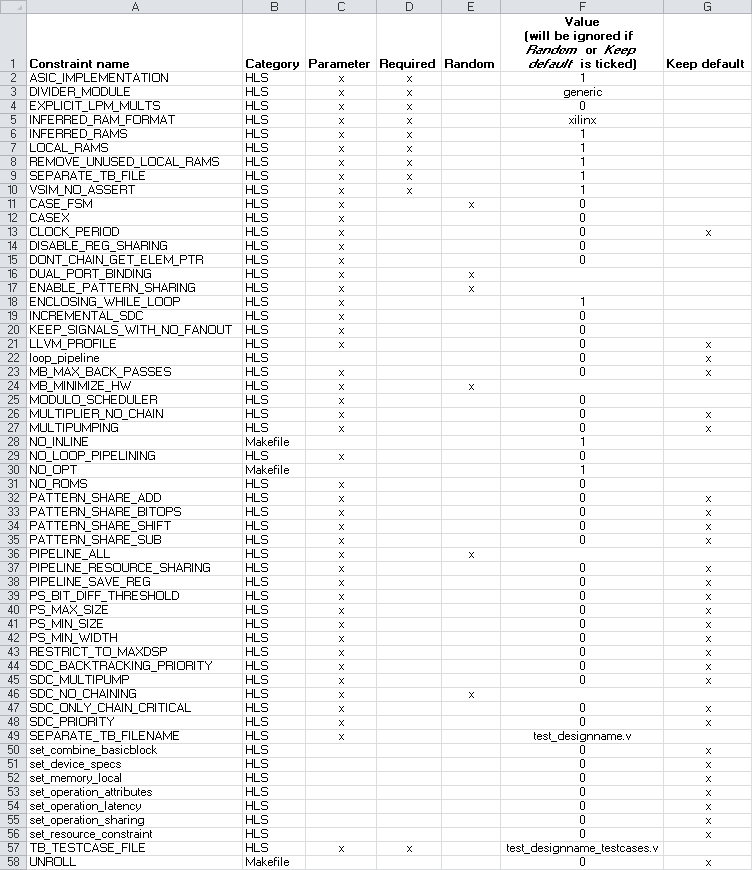
\includegraphics[width=\textwidth]{../figs/ConstraintGenerationSetup.png}
\caption{\label{fig:excelconstraintssetup}Setup of constraint file generation in Excel spreadsheet}
\end{figure}
Sheet 1 of the Excel file contains a \gls{csv} format of the constraint settings. The format of one \gls{csv}-string is:
\begin{verbatim}
parameterName,value,required,random,parameter,makefile,keepDefault
\end{verbatim}
Only the fields relevant for the parameter will be printed to the \gls{csv}, for instance the parameter \textit{CASE\_FSM} will print the line "\verb!CASE_FSM,random,parameter!", as this is the relevant fields for this parameter given the setup of the spreadsheet. Similar, the parameter \textit{NO\_OPT} will print the line "\verb!NO_OPT,1,makefile!", since this is a Makefile-parameter defined to have the value 1. The \gls{csv} format is copied from the Excel-file to a \gls{csv} file by using the headless tool \textit{convert-to} in libreoffice, with the command "\verb!libreoffice --headless --convert-to csv!". The \gls{csv}-file can then be read by the program generating constraint- and Makefiles. 

The program \textit{constraintGenerator.run} takes the filename of the \gls{csv}-file, the level parameter for the Makefile, and the designname as inputs, and returns the number of generated constraint files. This number is used in the framework-script to run the framework the correct number of times. This program is also written in the language C++, with reasoning similar to the one explained in \cref{subsec:llvmirparserprogram}. By parsing through the above described \gls{csv}-file, the program generate one constraint file and accompanying Makefile for each variation of the randomized constraint-parameters. Currently only parameters taking a 1-bit binary value is supported by the constraint generator program. This gives a total of $2^N$ designs, where \textit{N} is the number of randomized parameters. The constraints is set using a binary counter, meaning that for 3 randomized parameters, the first constraint file will have the values 0,0,0, the second file 0,0,1, the third file 0,1,0, and so on. The generated constraint and Makefiles are output to the directories \textit{constraintfiles} and \textit{makefiles} under the \textit{hls}-directory. The full code of the program generating constraint and Makefiles are listed in \cref{sec:constraintgeneratorsourcecode}.

\subsection{Report generating}
As the framework-script can be used to generate a large amount of designs, it is important to easily be able to collect the important data from all the generated reports. To ease the process of data collecting, the script collects the data from all designs and stores it in separate files. The data is collected using \textit{grep} commands, and the data is stripped of unnecessary text, using bash's substring replacement function, before output to files. The collected data is stored under the \textit{reports}-directory, with the file-names:
\begin{multicols}{2}
\textbf{From synthesis:}\\
\verb!register_count.rpt!

\textbf{From Layout:}\\
\verb!combinational_area.rpt!\\
\verb!noncombinational_area.rpt!\\
\verb!design_area.rpt!

\textbf{From power analysis:}\\
\verb!net_switching_power.rpt!\\
\verb!cell_internal_power.rpt!\\
\verb!cell_leakage_power.rpt!\\
\verb!total_power.rpt!

\textbf{Combined:}\\
\verb!all_results.rpt!
\end{multicols}

Each file contains the information specified by the filename. The corresponding design number is not included in the files, but the first line of each file contain results from design 0, the second line contain results from design 1, and so on. In the reports from power analysis, 5 values is stored at each line of the file, separated by commas. This is because the power analysis run five different power scenarios, each generating one result. The other files only contain a single value at each line. To simplify the process of importing the data into spreadsheets or other visualization-tools all files are joined horizontally into a single file, \textit{all\_results.rpt}. This means that each line will contain all values for a single design. The values in this file will be separated by tabs. This tidy file can be imported in Excel or other tools for generating graphs or compare data. Comparison could be made automatic if desired, but this is not implemented at this stage.

\section{\label{sec:runframework}Running the framework}
Before running the framework, some files need to be changed. The functional specification needs to be added to the file \textit{designName.c} and testcases for the simulation can be added to the file \textit{test\_designName\_testcases.v} under the directory \textit{sim/tb/}. In addition, the desired constraints need to be selected or filled out in the file \textit{constraints.xlsx} in the \textit{hls}-directory. To run the framework, the file \textit{HLSScript.sh} is executed from a shell. Depending on the design size, available licences, and number of randomized constraints, the run-time of the framework can be long. If the framework seems stuck on one of the tasks, check the log file, \textit{HLSscript.log}, for errors.


\chapter{Framework results}
The framework is tested using the reference design of a FIR-filter, described in \cref{subsec:refdesfir}. The source code of the filter, written in C, is listed in \cref{subsec:cfircode} in the appendix. The implemented FIR-filter has a 32-bit input, 16 taps and 64-bit output. The filter-coefficients are for simplicity defined to be the integers 1-16. By running this design through the framework, we will get multiple results. These results will be compared towards each other, but also towards the same FIR-filter implemented in Verilog directly. The source code of the Verilog implementation is listed in \cref{subsec:verilogfircode} in the appendix.

\section{\label{sec:firstrun}First test-run}
The first test-run were performed with 6 randomized constraints input to LegUp. Each of the constraints could take values 1 and 0, giving a total of $2^6=64$ combinations. The randomized constraints and the pattern of how the values are set is shown in \cref{tab:randomconstraint}.

\begin{table}
\tiny
    \begin{center}
    \begin{tabular}{l|cccccc}
     & & & \textbf{MB} & \textbf{ENABLE} & \textbf{DUAL} & \\
          &
          \textbf{SDC NO} & 
          \textbf{PIPELINE} & 
          \textbf{MINIMIZE} & 
          \textbf{PATTERN} & 
          \textbf{PORT} &
          \textbf{CASE} \\
        \textbf{Constraint}
           & \textbf{CHAINING}
           & \textbf{ALL}
           & \textbf{HW}
           & \textbf{SHARING}
           & \textbf{BINDING}
           & \textbf{FSM}
    \\ \midrule
    & 0 & 0 & 0 & 0 & 0 & 1 \\
    & 0 & 0 & 0 & 0 & 1 & 0 \\
    & 0 & 0 & 0 & 0 & 1 & 1 \\
    \textbf{Value} & \vdots & \vdots & \vdots & \vdots & \vdots & \vdots \\
    & &  &  &  &  &  \\
    & 1 & 1 & 1 & 1 & 1 & 0 \\
    & 1 & 1 & 1 & 1 & 1 & 1
    \\ \bottomrule
    \end{tabular}
    \caption{\label{tab:randomconstraint}Constraints and values for first run}
    \end{center}
\end{table}

This framework run only included HLS, simulation, and synthesis, as the layout and power estimation tools were not yet incorporated into the framework flow. Synthesis is run using a 32MHz clock and a 180nm cell library. A simple testbench generated by LegUp, with testcases similar to the ones listed in \cref{lst:tbcases}, were used for this run. 

The presented results are gathered from the synthesis reports. The generated Verilog for many of the constraint files synthesize into the exact same area consumption and. This indicates that some of the combinations are redundant. The results are shown in \cref{tab:hlsrun1dataresults}. As there are only 8 different results, only $log_2(8) = 3$ constraint parameters affect the design, the other will be don't-care constraints. By converting the design number to binary, the first row of the result table is shown in \cref{tab:dectobinconstraints}, a pattern can be seen and that the parameters \textit{PIPELINE\_ALL}, \textit{ENABLE\_PATTERN\_SHARING} and \textit{DUAL\_PORT\_BINDING} are don't care for the this design.

The area results are given in cell units, dynamic and total power are given in milliWatts (mW), and leakage power is given in nanoWatts (nW).


\begin{table}[hbtp]
    \centering
    \begin{tabular}{ccccc}
    & & \multicolumn{3}{c}{\textbf{Power}} \\
    \cline{3-5}
    \textbf{Design \#} & \textbf{Area} & \textbf{Dynamic} & \textbf{Leakage} & \textbf{Total} \\
    \toprule
    Verilog & 175517.771501 & 2.9522 & 13.2559 & 2.9522 \\
    9,11,13,15,25,27,29,31 & 542636.067533 & 1.1933 & 445.5482 & 1.1937 \\
    8,10,12,14,24,26,28,30 & 543715.713936 & 1.1909 & 442.7919 & 1.1913 \\
    41,43,45,47,57,59,61,63 & 570759.857112 & 1.3097 & 474.8710 & 1.3102 \\
    1,3,5,7,17,19,21,23 & 571069.521032 & 1.2792 & 467.3262 & 1.2797 \\
    0,2,4,6,16,18,20,22 & 574368.902419 & 1.2745 & 467.3031 & 1.2750 \\
    40,42,44,46,56,58,60,62 & 574468.505099 & 1.3100 & 475.3570 & 1.3105 \\
    33,35,37,39,49,51,53,55 & 598731.305489 & 1.3951 & 498.4164 & 1.3956 \\
    32,34,36,38,48,50,52,54 & 599552.442242 & 1.3949 & 500.0916 & 1.3954 \\
    \bottomrule
    \end{tabular}
    \caption{Results from first framework run}
    \label{tab:hlsrun1dataresults}
\end{table}

\begin{table}[hbtp]
    \centering
    \begin{tabular}{cccc}
    \textbf{Decimal} & \textbf{Binary}\\
    \toprule
    9 & 001001 \\
    11 & 001011 \\
    13 & 001101 \\
    15 & 001111 \\
    25 & 011001 \\
    27 & 011011 \\
    29 & 011101 \\
    31 & 011111 \\
    \bottomrule
    \end{tabular}
    \caption{Decimal to binary conversion shows the pattern in the constraints}
    \label{tab:dectobinconstraints}
\end{table}

\begin{figure}[hbpt]
\centering
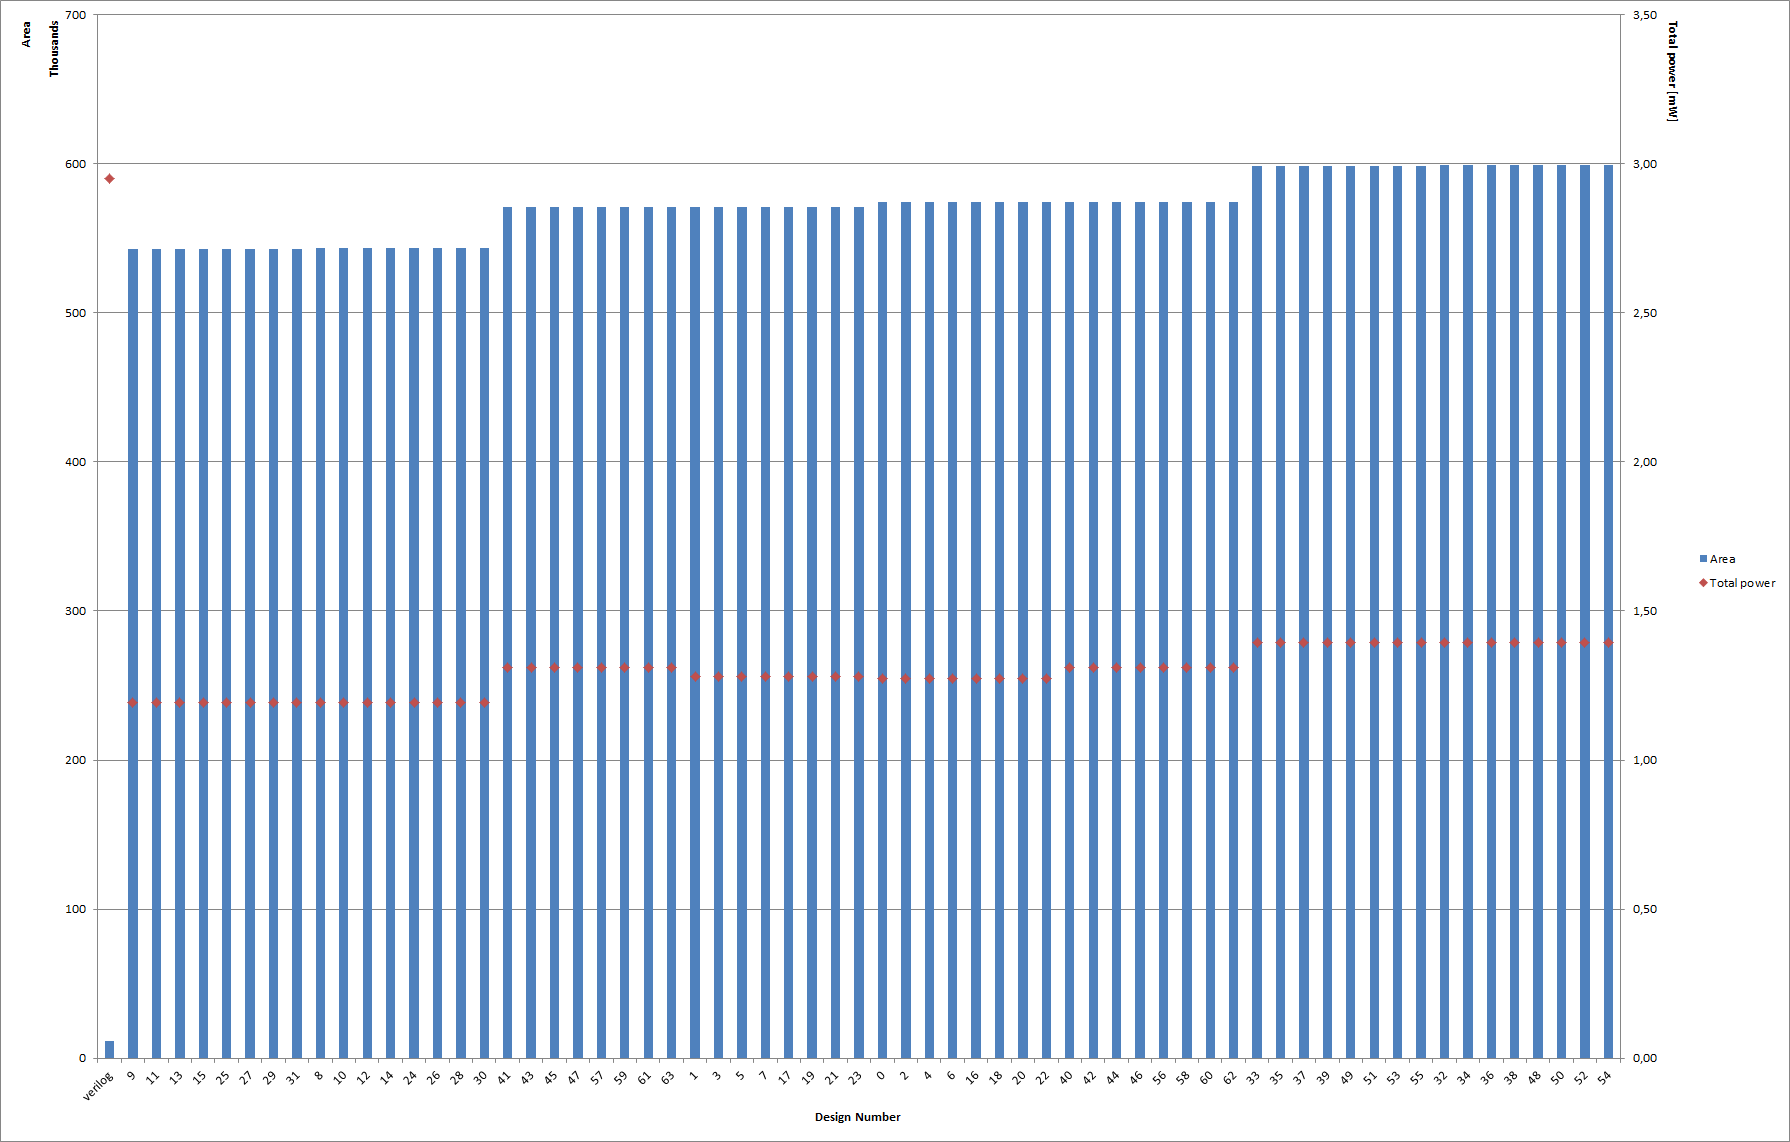
\includegraphics[width=\textwidth]{../figs/resultGraph.png}
\caption{\label{fig:resultgraphhlsrun1}Graph of results from first HLS run}
\end{figure}
The best result with regards to area is the ones with the parameters \textit{SDC\_NO\_CHAINING} set to 0, \textit{MB\_MINIMIZE\_HW} set to 1 and \textit{CASE\_FSM} set to 1. The best result with regards to total power consumption is the same as for area, just with \textit{CASE\_FSM} set to 0.

The results are visualized in \cref{fig:resultgraphhlsrun1}. It is clear from the graph that the concept is working as expected and that we get different result for different constraints. In \cref{fig:resultcomparisonhlsrun1}, the best area-result from the framework is compared towards the results from the same design written in Verilog directly. It is clear from the graph that the design written directly in Verilog is way better in terms of area consumption, it does not make sense that the estimated power consumption of the design in Verilog is much higher than the HLS-generated design.

\begin{figure}[hbpt]
\centering
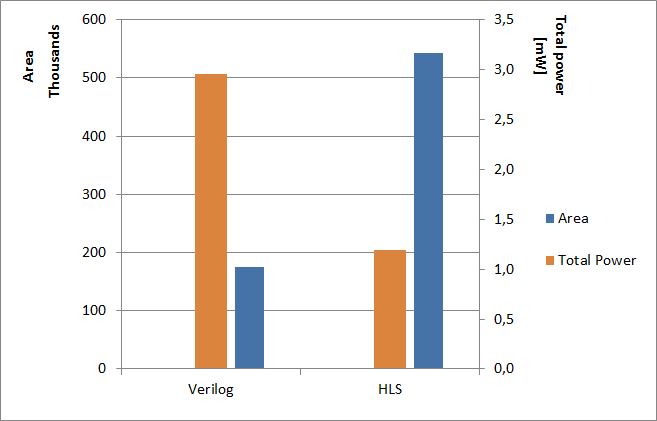
\includegraphics[width=0.75\textwidth]{../figs/resultComparison1.png}
\caption{\label{fig:resultcomparisonhlsrun1}Graph comparing framework generated design towards same design written in Verilog}
\end{figure}

\subsection{Handling unexpected results}
It seems strange that the area consumption of the design written in Verilog is just 32.3\% of the best result from LegUp, while the power consumption of the design written in Verilog is 247.4\% of the best result from LegUp. Typically a larger design will consume more power, as each of the components has leakage and static operation consumption. Notice that this results were obtained using a static power estimation tool, the amount of switching in gates and registers has not been taken into account. However, this unexpected result needed to be investigated further. The following steps were taken to ensure the quality of the results to be acceptable:

\begin{itemize}
    \item Check generated reports for misinterpreted data
    \item Look at schematic view of synthesized design to find errors
    \item Run HLS and synthesis once more to see if results deviates
\end{itemize}

None of the two first steps showed any errors. The designs are however too large to make any sense of the schematics, and due to to the limitation in setting signal sizes in the C-code, the HLS-generated Verilog designs scale down very poorly. The third step were performed on the same design, but with the clock relaxed from 32MHz to 16MHz. Changing the clock should not affect the design that much, but the synthesis will try to optimize the circuit to use the least amount of area, but still meet timing requirements. This time, only the constraints that had an impact on the design were included, generating 8 different designs. The result of the second run is shown in \cref{tab:resultgraphframeworkrun2} and in \cref{fig:resultgraphframeworkrun2}.
\begin{table}[hbtp]
    \centering
    \begin{tabular}{ccccc}
    & & \multicolumn{3}{c}{\textbf{Power}} \\
    \cline{3-5}
    \textbf{Design \#} & \textbf{Area} & \textbf{Dynamic} & \textbf{Leakage} & \textbf{Total} \\
    \toprule
    Verilog & 175531.077145 & 1.0961 & 291.4545 & 1.0964 \\
    3 & 736221.630958 & 3.0417 & 600.7903 & 3.0423 \\
    2 & 738362.360388 & 3.0424 & 603.0359 & 3.0430 \\
    0 & 766630.553023 & 3.1736 & 627.3008 & 3.1742 \\
    1 & 783120.518084 & 3.2230 & 641.3857 & 3.2236 \\
    7 & 796905.744222 & 3.0702 & 634.3779 & 3.0708 \\
    6 & 798087.595262 & 3.0693 & 635.5286 & 3.0699 \\
    4 & 830305.921961 & 3.2036 & 660.1381 & 3.2043 \\
    5 & 853504.409992 & 3.2898 & 681.0897 & 3.2905 \\

    \bottomrule
    \end{tabular}
    \caption{Results from second framework run.}
    \label{tab:resultgraphframeworkrun2}
\end{table}

\begin{figure}[hbpt]
\centering
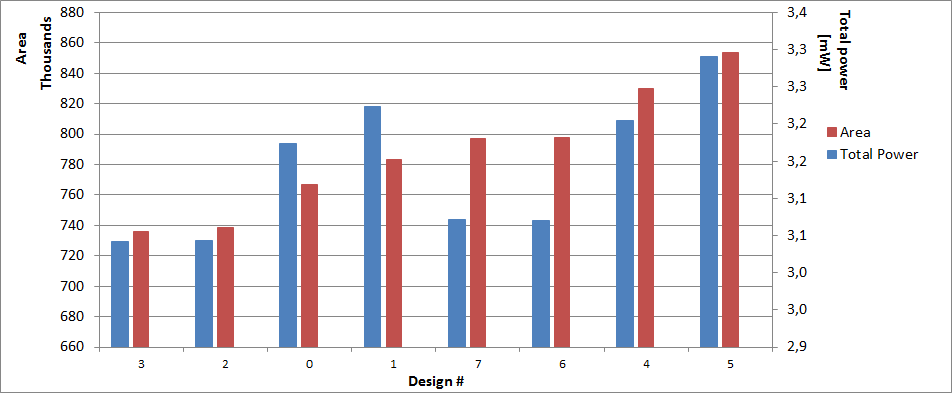
\includegraphics[width=\textwidth]{../figs/resultGraph2.png}
\caption{\label{fig:resultgraphframeworkrun2}Graph of results from second framework run}
\end{figure}

These results are a better match with our expectations. Both area and power has increased a bit for all HLS-generated designs. The reason for this is not known, but there could have been a bug in the design or a setting in the first run that generated odd results. When comparing the best HLS result towards the design written in Verilog, as shown in \cref{fig:resultcomparisonhlsrun2}, we see that the Verilog design has both lower area and power consumption, which is what would be expected.

\begin{figure}[hbpt]
\centering
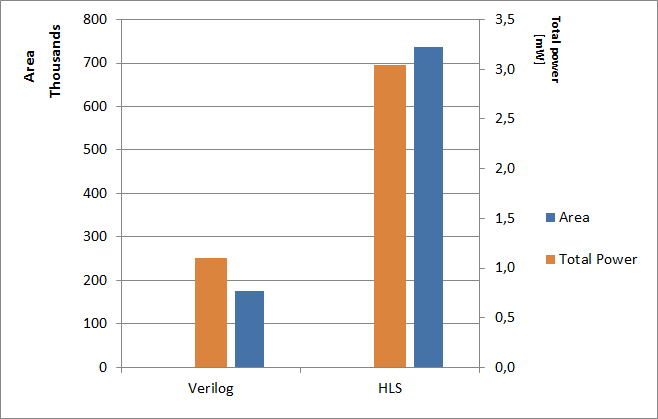
\includegraphics[width=0.75\textwidth]{../figs/resultComparison2.png}
\caption{\label{fig:resultcomparisonhlsrun2}Graph comparing framework generated design from second run towards same design written in Verilog}
\end{figure}

\section{Full tool-flow framework run}
The full tool-flow were incorporated into the framework, to see if more accurate power estimates shows a different result. With the full tool-flow, the area reports is gathered from layout instead of synthesis and the power estimates is gathered from power analysis. The full tool-flow is run using the same design as in \cref{sec:firstrun}, with only the three constraints that affected the output, again a total of 8 designs. Since the full tool-flow uses switching data from the simulation to perform power analysis, the testbench used had to be changed to get more switching values. The new testbench applies 1000 random inputs to the input \textit{inData} and waits for the flag \textit{iterationFinished} to be set before applying a new input. The full source code of this testbench is listed in \cref{subsec:firfiltertb}. The testbench for the design written in Verilog is almost exacly the same, just adapted to the correct signal names and instead of waiting for a flag, \textit{inData} is assigned a new value each 17 clock cycles. The area results are shown in \cref{tab:resultgraphareaframeworkrun2} and the power estimates are shown in \cref{tab:resultgraphpowerframeworkrun2}.

\begin{table}[hbtp]
    \centering
    \begin{tabular}{cccc}
    & \multicolumn{3}{c}{\textbf{Area}} \\
    \cline{2-4}
    \textbf{Design \#} & \textbf{Combinational} & \textbf{Non-combinational} & \textbf{Total} \\
    \toprule
    Verilog & 72818.22296 & 44647.6792 & 117465.9022 \\
    3 & 130953.7155 & 201114.5108 & 332068.2263 \\
    2 & 131389.4738 & 201114.5108 & 332503.9847 \\
    0 & 136182.8164 & 210973.9603 & 347156.7766 \\
    1 & 139276.3681 & 213895.2786 & 353171.6467 \\
    7 & 136262.6501 & 220468.2449 & 356730.8950 \\
    6 & 137237.2853 & 220468.2449 & 357705.5302 \\
    4 & 141315.4518 & 230327.6944 & 371643.1462 \\
    5 & 146770.7475 & 236170.3311 & 382941.0786 \\
    \bottomrule
    \end{tabular}
    \caption{Area results from framework run with full tool-flow}
    \label{tab:resultgraphareaframeworkrun2}
\end{table}

\begin{table}[hbtp]
    \centering
    \begin{tabular}{ccccc}
    & \multicolumn{4}{c}{\textbf{Power}} \\
    \cline{2-5}
    \textbf{Design \#} & \textbf{Net switching} & \textbf{Internal} & \textbf{Leakage} & \textbf{Total} \\
    \toprule
    Verilog & 0.365 & 1.760 & 100.340 & 2.125 \\
    2 & 1.214 & 5.157 & 281.820 & 6.371 \\
    3 & 1.236 & 5.270 & 273.940 & 6.507 \\
    6 & 1.184 & 5.484 & 293.960 & 6.669 \\
    0 & 1.273 & 5.518 & 292.400 & 6.792 \\
    1 & 1.279 & 5.517 & 307.760 & 6.797 \\
    7 & 1.255 & 5.567 & 267.960 & 6.822 \\
    4 & 1.238 & 5.696 & 308.180 & 6.934 \\
    5 & 1.269 & 5.771 & 327.280 & 7.041 \\
    \bottomrule
    \end{tabular}
    \caption{Power estimation results from framework run with full tool-flow.}
    \label{tab:resultgraphpowerframeworkrun2}
\end{table}

In \cref{fig:resultgraphframeworkrun3} the final area and power estimation results are visualized together. It is clear from the graphs that the concept works, as we get different results from the designs. These results are considered more accurate, as they use the reports from the chip layout for area, and power estimation using switching activity from simulation. Notice that compared to the results from synthesis, the area is actually cut by half, but the estimated power consumption has nearly doubled. This is because the layout tool can run optimizations on the design, decreasing the area, while the power estimates takes the dynamic switching activity into account, increasing the total power consumption. In \cref{fig:resultgraphpowerframeworkrun2}, the area and power estimates from the framework is compared against the same design written directly in Verilog. Here we see the same trend as shown in the synthesis results above, but the relationship between area and power consumption shows more resemblance.

\begin{figure}[hbpt]
\centering
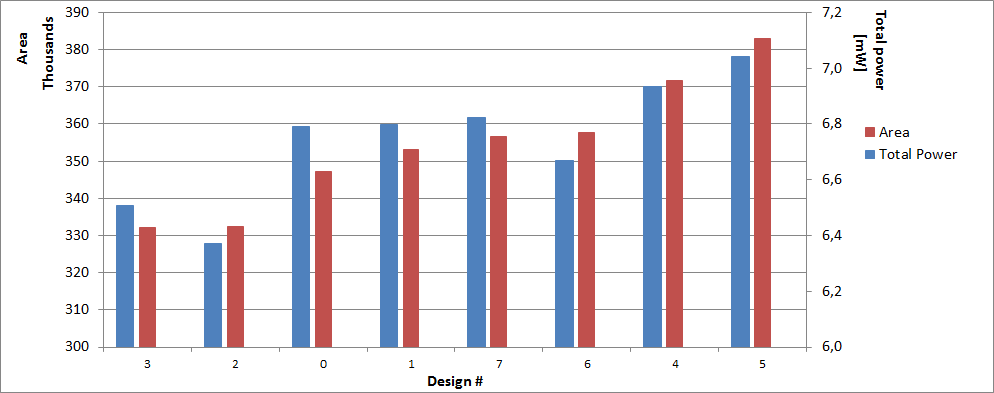
\includegraphics[width=\textwidth]{../figs/resultGraph3.png}
\caption{\label{fig:resultgraphframeworkrun3}Graph of results from framework with full tool-flow}
\end{figure}

\begin{figure}[hbpt]
\centering
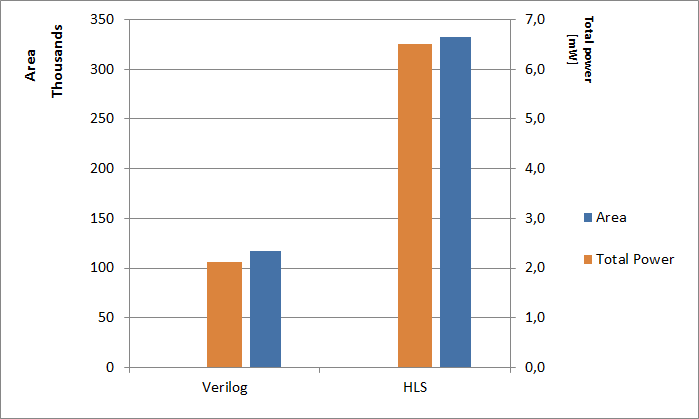
\includegraphics[width=0.75\textwidth]{../figs/resultComparison3.png}
\caption{\label{fig:resultcomparisonhlsrun3}Graph comparing framework generated design from full tool-flow towards same design written in Verilog}
\end{figure}

\cref{fig:resultgraphareaframeworkrun2} and\cref{fig:resultgraphpowerframeworkrun2} shows the distribution of area and power consumption within the designs. In the power graphs, lekage power is not shown as this is negligible compared to the other factors. The trend is the same in all the HLS generated designs, the larger portion of the area is consumed by non-combinational area. In the Verilog designs, the area distribution is inverted. This difference is what is expected from a FSM vs not-FSM design. In the power distribution graph we see that most of the power is consumed internally in the cells both in HLS generated designs and the Verilog design.

\begin{figure}[hbpt]
\centering
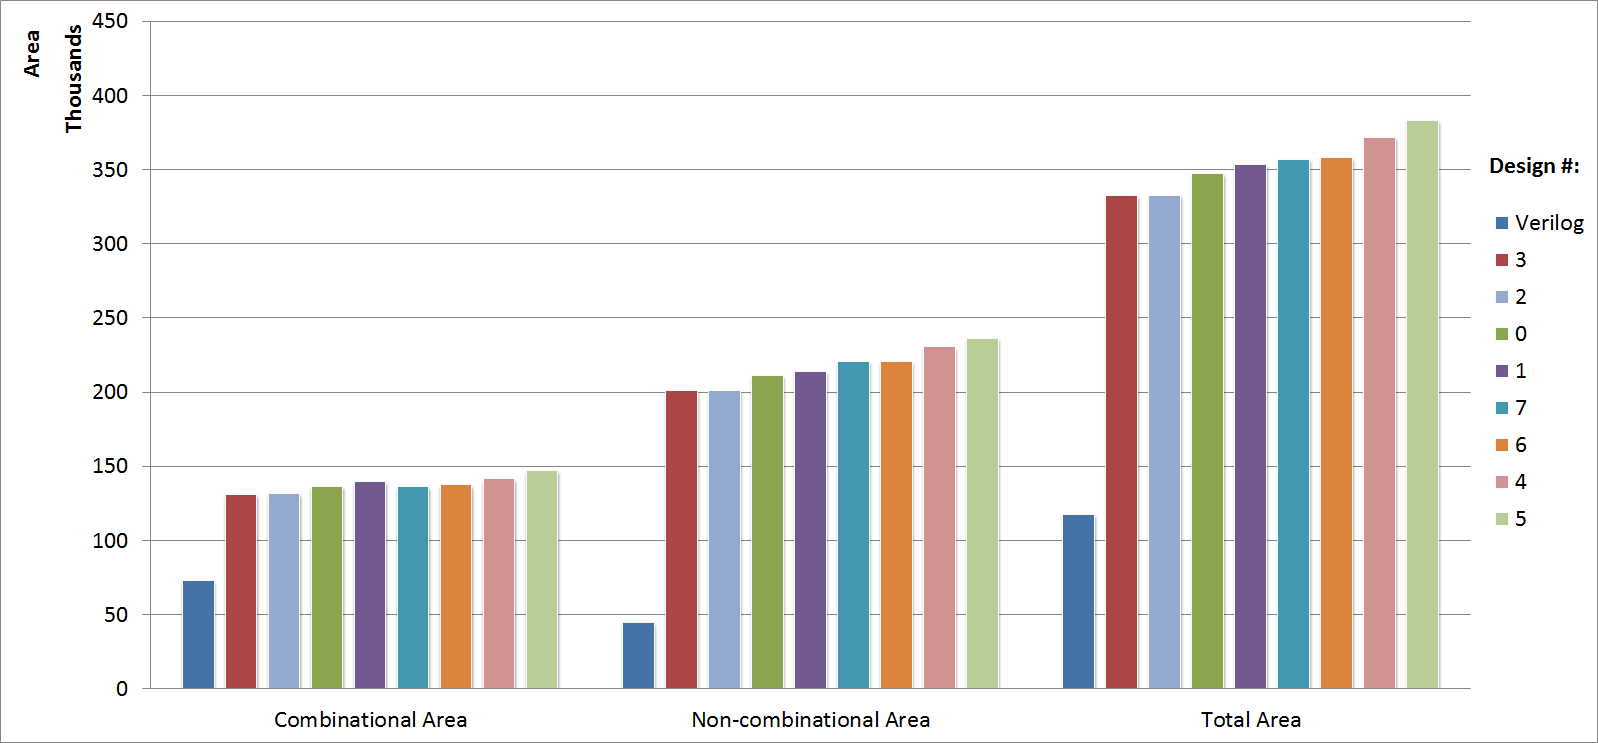
\includegraphics[width=\textwidth]{../figs/resultGraphAreaDistribution.png}
\caption{\label{fig:resultgraphareaframeworkrun2}Graph of area distribution of results from framework with full tool-flow}
\end{figure}

\begin{figure}[hbpt]
\centering
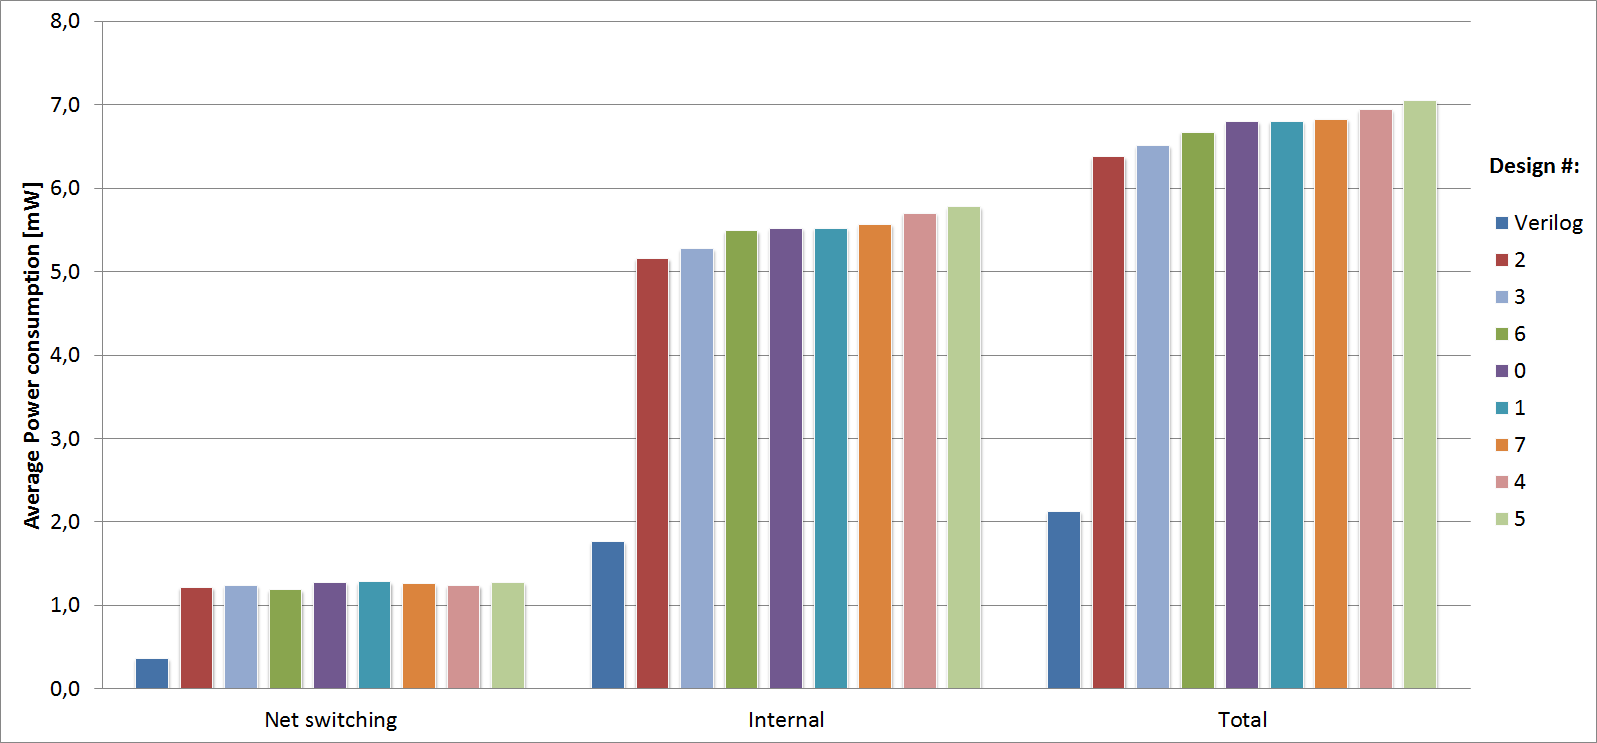
\includegraphics[width=\textwidth]{../figs/resultGraphPowerDistribution.png}
\caption{\label{fig:resultgraphpowerframeworkrun2}Graph of power distribution of results from framework with full tool-flow}
\end{figure}

Another interesting parameter to compare is the number if generated registers. For the implemented design, a minimum of 480 1-bit registers (\verb!INPUTSIZE*(TAPS-1)!) is needed for the shift register, the \textit{sr}-array. The number of registers, gathered from the synthesis reports, is shown in \cref{tab:resultregistercount}. 

\begin{table}[hbtp]
    \centering
    \begin{tabular}{cc}
    \textbf{Design \#} & \textbf{Registers} \\
    \toprule
    Verilog & 480 \\
    0 & 2311 \\
    1 & 2343 \\
    2 & 2203 \\
    3 & 2203 \\
    4 & 2523 \\
    5 & 2587 \\
    6 & 2415 \\
    7 & 2415 \\
    \bottomrule
    \end{tabular}
    \caption{Number of used registers for each design}
    \label{tab:resultregistercount}
\end{table}
\section{Bugs in the generated design}
To avoid the generating of a global memory controller, the flag \textit{NO\_INLINE} had to be set to 0 in the Makefile. This introduces two bugs in the generated Verilog; firstly, the signal generated from the parameter \textit{done} is not sampled after the first time, making the program run forever, secondly the statement \verb!products[0] = inData * 1! is only evaluated on the first iteration of the loop, meaning all outputs from the FIR-filter (except the first one) will have a deviation from the correct result, corresponding to \verb!correctResult - inData + firstInData!. From the generated LLVM IR code it looks like the first bug occurs because the comparison of the input \textit{done} being performed in another state than where it is used as loop exit-condition. In the same state, \textit{inData} is sign-extended, as it is a 32-bit variable being assigned to a 64-bit variable. Both these results are stored to temporary registers for use later, as shown below. From the simulation, it can be seen that this particular state is not visited again when the loop has been entered.
\lstset{language=llvm,style=LLVMstyle}
\begin{lstlisting}
%6 = icmp eq i32 %done, 0
%7 = sext i32 %inData to i64
\end{lstlisting}
These bugs are not critical to this case, as both bugs will be identical to each design. As this results is only supposed to show that the concept works, it is not critical that the generated results are accurate, as long as they are accurate relative to each other.
\section{Path and hold violations}
Some of the designs reports violating path length and hold times in synthesis. For a real circuit this would be a problem. To get rid of these violations, the target clock speed during synthesis could be decreased to something below the maximum frequency of the design. However, the clock speed is most of the time the only thing you cannot change in your design, and design compiler will try to create the circuit that meets timing. If timing is not met, the circuit description should be changed. This means that from our methodology, we will generate many circuits and only the ones that meet timing will be presented as an accepted solution. Ideally, the framework would implement a feedback loop, but for the sake of this proof-of-concept, a long list of solutions are produced and only the best ones are selected.

\section{LegUp specific code optimization}

When going trough the register-count from synthesis, it were noticed that the HLS generated designs implemented both the array \textit{sr} and \textit{products} as RAM modules using registers, while in the design written directly in Verilog, the \textit{sr}-array is the only signal using registers. When looking at the following snippet from the FIR-filter source code, listed in \cref{subsec:cfircode}:
\lstset{language=C,style=CStyle}
\begin{lstlisting}
for (int k = 1; k < TAPS ; k++){
    products[k] = sr[k-1] * (k+1);
}
sum = sum + products[i];
\end{lstlisting}
it can easily be seen that this is functionally equivalent to:
\begin{lstlisting}
sum = sum + (sr[i-1] * (i+1));
\end{lstlisting}
This connection should be made either in the compiler or in LegUp, but it were clearly missed. If we also substitute the code:
\begin{lstlisting}
products[0] = inData * 1;
sum = products[0];
\end{lstlisting}
with:
\begin{lstlisting}
sum = inData * 1;
\end{lstlisting}
the whole \textit{products}-array can be removed. When running this optimized code through the framework, the result is much better than without these optimizations. \cref{tab:resultsframeworkrun3} shows the results from the framework run of design 2, the best design with regards to power consumption from the second framework run.

\begin{table}[hbtp]
    \centering
    \begin{tabular}{lr}
    \multicolumn{2}{c}{\textbf{Synthesis}} \\
    \toprule
    Total Area & 358587.628093 \\
    \hline
    Net Switching Power & 0.1340 mW \\
    Internal Power & 1.3203 mW \\
    Leakage Power & 283.1053 nW \\
    \hline
    Total Power & 1.4546 mW \\
    \hline
    Register count & 899 \\ 
    \bottomrule
    & \\
    \multicolumn{2}{c}{\textbf{Layout}} \\
    \toprule
    Combinational Area & 72482.256207 \\
    Non-combinational Area & 82070.787659 \\
    \hline
    Total Area & 154553.043866 \\
    \bottomrule
    & \\
    \multicolumn{2}{c}{\textbf{Power analysis}} \\
    \toprule
    Avg. Net Switching Power & 0.604 mW \\
    Avg. Internal Power & 2.413 mW \\
    Avg. Leakage Power & 105.500 nW \\
    \hline
    Avg. Total Power & 3.018 mW \\
    \bottomrule
    \end{tabular}
    \caption{Results of best design from framework run with optimized C-code.}
    \label{tab:resultsframeworkrun3}
\end{table}
The results from the optimized code gives the overhead shown in \cref{tab:overheadframeworkrun3}. These overhead percentages corresponds more with the typical overhead of 30-40\% in HLS tools.
\begin{table}[hbtp]
    \centering
    \begin{tabular}{lr}
    \multicolumn{2}{c}{\textbf{Overhead}} \\
    \toprule
    %Synthesis area & 183056.550948 (104.29\%)
    %Synthesis power & 0.3582mW (32.67\%)
    %Register count & 419 1-bit registers (87.29\%)
    Layout area & 37087.141666 (31.57\%) \\
    Average power & 0.893mW (42.02\%) \\
    Register count & 419 (87.29\%) \\
    \bottomrule
    \end{tabular}
    \caption{Results of best design from framework run with optimized C-code.}
    \label{tab:overheadframeworkrun3}
\end{table}


\chapter{Discussion}

The alterations done to LegUp to get Verilog output suitable for ASIC implementation has limited the use of many features of the higher level of abstraction in C. This put large constraints on how you can write your C-code if you want to run it through the framework. Especially the pointer and related array-support should be working. An alternative to bring these features back would be to re-introduce the top-module that instantiates the \textit{main}-module and the \textit{memory\_controller}- module and pass all inputs and outputs directly through the top and to the \textit{main}-module. This would work after the implementation of outputs from parameters and the streaming port feature. The downside of this approach is that the memory controller will bring back some extra overhead to the design. An alternative solution would be to further alter the libraries of LegUp, to make sure all RAMs are implemented as local RAMs. 

The framework has been created to be easily configurable and adaptable if it is desirable to add functionality. For this proof-of-concept, only constraints set on the HLS process in LegUp has been used. It could however be useful to add other parameters to the framework, to control other parts of the tool-flow. Examples could be to run synthesis using different clock-speeds, or to specify optimization goals, like minimum area or maximum speed, for synthesis and layout. This would generate an even wider pool of designs to decide from, increasing the chance of getting the very best design. The downside of including more parameters into the framework is the exponential increase in the number of designs and accompanying tool-flow run-time. If all possibilities of 50 different constraints, each having two possible values, should be explored, a total of $2^{50} = 1~125~899~906~842~624$ (over 1 quadrillion) designs would have to be run through the tool-flow. If the tool-flow used 1 minute to process each design, the run-time for the framework would end up at 2.142 billion years. In practice, the designer is therefore required to select a few parameters that he puts his belief in, and hope this gives one of the best possible results.

By comparing the best-case design towards the worst-case design, a potential area saving of 50872.8523 and power sawing of 0.670 mW is achieved. This corresponds to a decrease in area of 13.28\% and a decrease in power consumption of 9.52\%. Compared to the design written directly in Verilog, the best-case area is 282.69\% and power consumption is 331.34\% of the results achieved in the Verilog design. An overhead of almost 200\% is not a great result, but the idea here is not to get a comparable result, rather to show that the concept works and can be used for a framework for architectural exploration. This goal has been achieved, as we get varied outputs depending on the given HLS constraints.

Even though the desired proof-of-concept has been shown, the changes made to LegUp to achieve a acceptable Verilog output suitable for ASIC implementation, has generated many limitations and special cases with regards to how the functional specification can be written. Originally the input were ANSI-C, supporting functions, arrays, structs, global variables, floating point, and pointers. When using this adaption of LegUp for generating ASIC-compliant Verilog, only functions and partially arrays seem to work correctly. Most of these limitations can probably be overcome by altering the libraries further, but this will be time consuming.

\section{Advances in LegUp since last release}
From the GIT repository of LegUp, it can be seen that many new features have been and still are being implemented for the next release version of LegUp. The current version (4.0), were released in August 2015. One of the more interesting features from the views of this project is the implementation of streaming inputs and outputs. Even though this has been implemented in this project as well, a native implementation from the developers can be more thoroughly tested and have more functionality than the one implemented here. However, it is still uncertain if a good way of producing multiple output-signals have been implemented. In another commit it is mentioned that it will be possible to mark a RAM as external, making it possible to pass pointers as arguments into the top-level function. These features are exciting news from the perspective of this thesis, as it can look like the developers implements more things useful for ASIC hardware development.
\chapter{Conclusion}
\label{chp:conclusion} 
This thesis has presented a solution for adapting the \gls{hls}-tool LegUp, to make the tool produce Verilog-output suitable for synthesis towards \gls{asic} architectures. In addition to this, a framework for architectural exploration of digital hardware has been developed, using LegUp to increase the abstraction-level of a functional description. The framework is capable of generating a wide variety of architectural implementations of the given functional specification, using randomized constraints in the \gls{hls}-flow to get varying output. Each of the designs generated by \gls{hls} will automatically be simulated and synthesized, before layout and power analysis is performed on the design. The framework will generate reports containing relevant parameters, like area, power estimates, speed, and register count, for each design. The reports allow for the designer to easily compare the designs and select the one best suited based on the specification.

To ensure the functionality of the framework, a proof of concept has been conducted, using a FIR-filter as the reference design. The results from the framework shows that three of the six randomized constraint used, had an impact on the generated design. This gave a total of 8 architectural variations. By comparing the best and worst of the generated architectural variations, a decrease in area of 13.28\% and a decrease in power consumption of 9.52\% could be achieved. These results indicate that the proof of concept works.

When running the framework, some problems and bugs in the generated design were observed. Some of these were related to how the adaption of LegUp is performed, while some could be bugs in LegUp or the tool-flow. It is also an element of concern that the way you write your functional specification can affect the generated designs greatly. The compiler or LegUp should be able to optimize away any parts of the code that is obsolete. If this concept is to be used at a professional level, it is vital that all parts of the framework generate error-free results. 

The overhead in area and power estimates are still high, with a best observed result of 31.57\% in terms of area and 42.02\% in terms of average power consumption. The overhead is especially high in the non-optimized functional specification used in most of \cref{chp:frameworkresults}, where the generated overhead in area and power consumption is close to 200\%. This overhead needs to be reduced, or at least ensured to stay at a constant percentage, if the \gls{hls}-tool is to be used in the framework.

The final conclusion is that the concept have been shown and is generating varying results in the proof of concept. As only one design was used during the proof of concept, it cannot be  It is also shown that LegUp, in the adapted version described in this thesis, can be used in a framework for architectural exploration. However, much more effort should be put into verification and testing of all parts of the tool-flow, to ensure all bugs and potential errors are eliminated before using it for any commercial purpose.
\section{Future work}
\label{sec:futurework} 
\subsection{Abstraction level}
During the process of adapting LegUp, to make the generated Verilog more suitable for \gls{asic} implementation, much of the higher level of abstraction originally supported by LegUp, have been lost. The limitation on how the code can be written, reduces the usefulness of the framework. It would increase the value of the framework greatly if a better solution to the resolved issues can be found, or another method can be used to bring back the desired functionality from \gls{ansi}-C.

\subsection{Resolving bugs}
In \cref{sec:designbugs} two bugs that were noticed in simulation have been described. For the framework to be useful, the generated designs should be bug-free, given that no bugs are present in the functional description. It should be put some effort into figuring out what is creating these bugs, and find a solution to avoid that these, and other bugs are generated in future designs.

\subsection{Eliminating RAM states}
In \cref{subsec:removerams}, a method of removing local \gls{ram}s generated by using the keyword \textit{volatile} for input-parameters was described. This method of removing the \gls{ram}s does not seem to remove the states designated to the allocation and storing to the generated \gls{ram}s. An example of this can be seen by looking at the generated state machine in \cref{fig:verilogfsm}. Here the states \textit{1} and \textit{2} does not perform any operations, as they were dedicated to allocation of, and storing to, the generated \gls{ram}. A method of removing these states should be added to the altered version of LegUp. Having states in the \gls{fsm} that do not perform any operation, only leads to extra clock-cycles being used to produce the desired output, decreasing the overall speed of the circuit.

\subsection{Advances in LegUp since last release}
For this thesis, the current release version (4.0) of LegUp, released in August 2015, was used. LegUp's normal release cycle is roughly once a year \cite{legupfaq}. From the GIT repository of LegUp \cite{legupgit}, it can be seen that many new features have been, and still are being, implemented for the next release version of LegUp. One of the more interesting features from the views of this thesis is the implementation of streaming inputs and outputs. Even though this has been implemented in this thesis as well, a native implementation from the developers can be more thoroughly tested and have more functionality than the one implemented here. However, it is still uncertain if a good way of producing multiple output-signals have been implemented. In another commit it is mentioned that it will be possible to mark a \gls{ram} as external, making it possible to pass pointers as arguments into the top-level function. These features are exciting news from the perspective of this thesis, as it can look like the developers implements more things useful for \gls{asic} hardware development. The upcoming release of LegUp, should be explored to see if any of the new features is useful for the concept described in this thesis. 

\subsection{Automatic code-optimization}
The overhead in both area and power-consumption could be reduced greatly by manually optimizing the code input to the framework, as described in \cref{sec:codeoptimization}. This is a huge drawback of the framework, as it forces the designer to keep focus on writing the code in the most correct way, instead of focusing on writing the correct functional specification. The task of optimizing the input should be left to the compiler or \gls{hls}-tool. It would be strongly beneficial if a solution could be implemented to ensure that the code is optimized correctly.

\subsection{Incorporating Nordic Semiconductors DDVC}
The last objective described in \cref{sec:projectobj} have not been considered in this thesis, as the work with providing a functional framework and creating the proof of concept took all of the available time. It would still be interesting to see if the incorporation of Nordic Semiconductors \gls{ddvc} into the Verilog-generating libraries of LegUp will reduce the overhead of the tool.
%% include here the other chapters

\renewcommand*{\bibname}{References}
%\bibliographystyle{plain}
\bibliographystyle{plainnat}
\bibliography{main}

%% Uncomment the following if you have any appendix
 \appendix
 \addtocontents{toc}{%
  \protect\vspace{1em}% 
  \protect\noindent \bfseries \appendixtocname\protect\par
  \protect\vspace{-.5em}%
 }
 \renewcommand{\chaptername}{\appendixname}
%% include below possible appendices (chapters)

%\chapter{Source code listings}
\section{\label{sec:sourcecode}FIR-filter reference design}
\subsection{\label{subsec:cfircode}C source code}
\lstset{language=C,style=CStyle}
\begin{lstlisting}
#include <stdint.h>

#define INPUTSIZE 32
#define TAPS 16

int main(int done, int inData, volatile long long int __out_outData) {

  int sr[TAPS-1] = {0};
  long long int products[TAPS] = {0};
  long long int sum = 0;
  while(done == 0){
    products[0] = inData * 1;
    sum = products[0];
    for (int i = 1; i < TAPS ; i++){
      for(int j = TAPS-1; j > 0; j--){
        sr[j] = sr[j -1];
      }
      sr[0] = inData;
      for (int k = 1; k < TAPS ; k++){
        products[k] = sr[k-1] * (k+1);
      }
      sum = sum + products[i];
    }
    __out_outData = sum;
  }
  return 0;
}
\end{lstlisting}
\clearpage
\subsection{\label{subsec:cfircode2}Optimized C source code}
\begin{lstlisting}
#include <stdint.h>

#define INPUTSIZE 32
#define TAPS 16

int main(int done, int inData, volatile long long int __out_outData) {
  int sr[TAPS-1] = {0};
  long long int sum = 0;
  while(done == 0){
    sum = inData;
    for (int i = 1; i < TAPS ; i++){
      for(int j = TAPS-1; j > 0; j--){
        sr[j] = sr[j -1];
      }
      sr[0] = inData;
      sum = sum + sr[i-1] * (i+1);
    }
    __out_outData = sum;
  }
  return 0;
}
\end{lstlisting}
\clearpage
\subsection{\label{subsec:verilogfircode}Verilog source code}
\lstset{language=Verilog,style=VerilogStyle}
\begin{lstlisting}
module fir (
    clk,
    reset,
    dataIn,
    dataOut
  );
  parameter WIDTH = 32;
  parameter DEPTH = 16;

		
  input clk, reset;
  input signed [WIDTH-1:0] dataIn;
  output wire signed [2*WIDTH-1:0] dataOut;
  integer i, j, k;
  reg signed [WIDTH-1:0] sr [DEPTH-2:0];
  reg signed [2*WIDTH-1:0] products [DEPTH-1:0];
  reg signed [2*WIDTH-1:0] sum;

  always @( posedge clk or posedge reset ) begin
    if( reset == 1) begin
      sum = 0;
    end
    else begin
	  for(i = DEPTH-2; i > 0; i=i-1) begin
        sr[i] <= sr[i-1];
      end
	  sr[0] <= dataIn;
    end
  end

  always @(*) begin
	products[0] = dataIn * 1;
    for (j = 1; j < DEPTH ; j=j+1) begin
      products[j] = sr[j-1] * (j+1);
	end
  end

  always @(*) begin
    sum = products [0];
    for (k = 1; k < DEPTH ; k=k+1) begin
      sum = sum + products[k];
	end
  end
	
  assign dataOut = sum;
	
endmodule
\end{lstlisting}
\clearpage
\subsection{\label{subsec:firfiltertb}Testbench for FIR-filter}
\lstset{language=Verilog,style=VerilogStyle}
\begin{lstlisting}
`timescale 1 ns / 1 ns
module test_fir
(
);

reg  clk;
reg  reset;
reg  start;
wire [63:0] return_val;
wire  finish;
reg  memory_controller_waitrequest;
reg [31:0] arg_done;
reg [31:0] arg_inData;
wire [63:0] arg_outData;
wire  arg_outData_valid;
wire  iterationFinish;


fir u_fir (
	.clk (clk),
	.reset (reset),
	.start (start),
	.finish (finish),
	.memory_controller_waitrequest (memory_controller_waitrequest),
	.return_val (return_val),
	.arg_done (arg_done),
	.arg_inData (arg_inData),
	.arg_outData (arg_outData),
	.arg_outData_valid (arg_outData_valid),
	.iterationFinish (iterationFinish)
);

// Clock generation
initial 
    clk = 0;
always @(clk)
    clk <= #10 ~clk;

initial begin
@(negedge clk);
reset <= 1;
@(negedge clk);
reset <= 0;
start <= 1;
@(negedge clk);
start <= 0;
end

always@(finish) begin
    if (finish == 1) begin
        $display("At t=%t simulation finished", $time);
        $display("Cycles: %d", ($time-50)/20);
        $finish;
    end
end

initial begin
memory_controller_waitrequest <= 1;
@(negedge clk);
@(negedge clk);
memory_controller_waitrequest <= 0;
end

// Custom testcases:     
  initial begin
    arg_inData = 32'b0; 
		arg_done = 32'b0;
  end 
	
	initial  
  begin : TEST_CASE 
		@(posedge reset)
		repeat (1000) begin 
			@(negedge clk); 
			arg_inData = $random; 
			@(posedge iterationFinish); 
		end	
		$display("Finished applying inData\n");
		arg_done = 32'b1;
		#100ns
		$finish;
  end 

endmodule 
\end{lstlisting}
%\section{\label{lst:llvmirparserprogramcode}LLVM IR Parser program}
\lstset{language=C++,style=Cstyle}
\begin{lstlisting}
#include <iostream>
#include <fstream>
#include <string>
#include <algorithm>
#include <vector>
#include <set>
using namespace std;

int main(int argc, char *argv[]) {

    // Check for correct amount of arguments
    if (argc < 3) {
        cout << "Missing output file argument\n";
        if (argc < 2) {
            cout << "Missing input file argument\n";
        }
        cout << "Arguments should be at the form: inputfile outputfile\n";
        return 1;
    }

    vector<string> sources;
    vector<string> targets;
    vector<int> labels;

    ifstream inFile(argv[1]);
    ofstream outFile(argv[2]);

    if (inFile.is_open()) {
        cout << "inFile opened successfully\n";
        string line;
        string searchStringStores = "  store";
        string searchStringMain = "define";
        string labelString = "; <label>:";
        string whitespace = " ";
        int inMain = false;
        int currLabel = 0;
        bool isTarget = false;
        // Read file line by line
        while (getline(inFile, line)) {
            // Only consider lines staring with "  store"
            if (line.compare(0, searchStringMain.length(), searchStringMain) ==
                    0 &&
                !inMain) {

                size_t found = 0;
                do {
                    found = line.find(whitespace, found + 1);
                } while (line.compare(found + 1, 1, "@") != 0);
                if (line.compare(found + 1, 6, "@main(") == 0) {
                    inMain = true;
                    currLabel = 0;
                }
            } else if (line.compare(0, labelString.length(), labelString) ==
                       0) {
                currLabel = atoi(line.substr(10, 3).c_str());
            } else if (line.compare(0, searchStringStores.length(),
                                    searchStringStores) == 0 &&
                       inMain) {

                // Remove commas from line
                line.erase(std::remove(line.begin(), line.end(), ','),
                           line.end());

                // Remove leading and trailing whitespaces
                line.erase(
                    line.begin(),
                    std::find_if(line.begin(), line.end(),
                                 bind1st(std::not_equal_to<char>(), ' ')));

                // Split line at whitespace

                size_t found = line.find(whitespace);
                while (found != string::npos) {
                    size_t foundNext = line.find(whitespace, found + 1);

                    // Only store words staring with a % sign
                    if (line.compare(found + 1, 1, "%") == 0) {
                        string substring =
                            line.substr(found + 2, foundNext - found - 2);
                        if (isTarget == true) {
                            targets.push_back(substring);
                            labels.push_back(currLabel);
                            isTarget = false;
                        } else {
                            sources.push_back(substring);
                            isTarget = true;
                        }
                    }
                    found = foundNext;
                }
                if (sources.size() > targets.size()) {
                    sources.pop_back();
                    isTarget = false;
                }
                if (line.compare(0, 1, "}") == 0) {
                    inMain = false;
                }
            }
        }
        inFile.close();
    }

    else
        cout << "Unable to open input file\n";

    if (outFile.is_open()) {
        cout << "outFile opened successfully\n";
        set<string> done;

        // Iterate through all found stores and check for assignment connections
        for (int i = 0; i < targets.size(); ++i) {
            for (int j = 0; j < targets.size(); ++j) {
                if (targets[i] == targets[j] && i != j &&
                    done.find(sources[i]) == done.end() &&
                    sources[i].find("__out_") == 0) {
                    done.insert(sources[j]);
                    string sigName = sources[i];
                    // Only print parameters defined as outputs
                    if (sigName.find("__out_") == 0) {
                        sigName = sigName.substr(6, std::string::npos);
                        outFile << sigName << " " << sources[j] << " "
                                << labels[j] << " " << labels[i] << " "
                                << targets[i] << "\n";
                    }
                }
            }
        }
        outFile.close();
    }

    else
        cout << "Unable to open output file\n";

    return 0;
}

\end{lstlisting}
\clearpage
\section{\label{sec:validsinglssourcecode}Generating valid signals}
\lstset{language=C++,style=Cstyle}
\begin{lstlisting}
// Add each driving signal from source as a driver of the target
// signal.
// Also generate conditions for valid signals and drive these.
for (uint j = 1; j < sourceSig->getNumDrivers(); j += 2) {
    if (sourceSig->getDriver(j)->getName().compare(
            targetSig->getName()) != 0) {
        targetSig->addCondition(sourceSig->getCondition(j),
                                sourceSig->getDriver(j));
        if (j + 1 < sourceSig->getNumDrivers()) {
            targetSig->addCondition(sourceSig->getCondition(j + 1),
                                    sourceSig->getDriver(j + 1));
        }
        if (sourceSig->getCondition(j)->isOp()) {
            validSig->addCondition(sourceSig->getCondition(j), ONE);
            if (j + 1 < sourceSig->getNumDrivers()) {
                validSig->addCondition(
                    sourceSig->getCondition(j + 1), ONE);
            }
            if (sourceSig->getNumDrivers() - 1 < 2) {
                // Adds deassertion of validSig if only single
                // conditions are present.
                validSig->addCondition(
                    rtl->addOp(RTLOp::Not)
                        ->setOperands(sourceSig->getCondition(j)),
                    ZERO);
            } else if (sourceSig->getNumDrivers() - 1 < 3 ||
                       j == 1) {
                notValid->setOperands(
                    rtl->addOp(RTLOp::Not)
                        ->setOperands(sourceSig->getCondition(j)),
                    rtl->addOp(RTLOp::Not)->setOperands(
                        sourceSig->getCondition(j + 1)));
            } else if (sourceSig->getNumDrivers() - j > 1) {
                RTLSignal *notValid1 =
                    rtl->addOp(RTLOp::And)->setOperands(
                        rtl->addOp(RTLOp::Not)->setOperands(
                            sourceSig->getCondition(j)),
                        rtl->addOp(RTLOp::Not)->setOperands(
                            sourceSig->getCondition(j + 1)));
                RTLSignal *notValid2 =
                    rtl->addOp(RTLOp::And)
                        ->setOperands(notValid->getOperand(0),
                                      notValid->getOperand(1));
                notValid->setOperands(notValid1, notValid2);
            } else {
                RTLSignal *notValid1 =
                    rtl->addOp(RTLOp::And)
                        ->setOperands(notValid->getOperand(0),
                                      notValid->getOperand(1));
                notValid->setOperands(
                    notValid1, rtl->addOp(RTLOp::Not)->setOperands(
                                   sourceSig->getCondition(j)));
            }
        }
    }
}
// Adds deassertion of validSig if multiple conditions are present.
if (notValid->getNumOperands() > 1) {
    validSig->addCondition(notValid, ZERO);
}
\end{lstlisting}
\clearpage
\section{\label{sec:iterationfinishsourcecode}Adding iterationFinish flag}
\begin{lstlisting}
RTLSignal *interationFinish = rtl->addOutReg("interationFinish");

connectSignalToDriverInState(interationFinish, ONE, (--fsm->end())->getPrevNode());
interationFinish->addCondition(rtl->addOp(RTLOp::Not)->setOperands(interationFinish->getCondition(0)), ZERO);
\end{lstlisting}

\section{\label{sec:tbgenerationsourcecode}Testbench generator source code}
\begin{lstlisting}
RTLModule *t = m->addModule("main", "main_inst");
if (LEGUP_CONFIG->getParameterInt("ASIC_IMPLEMENTATION")) {
  RTLModule *rtl = alloc->getModuleForFunction(alloc->getModule()->getFunction("main"));
  if (rtl->getName().compare("main") == 0) {
    for (RTLModule::const_signal_iterator i = rtl->port_begin(), e = rtl->port_end(); i != e; ++i) {
      const RTLSignal *s = *i;
      RTLSignal *d;
      string type = s->getType();
      if (!type.empty()) {
        if (type.compare(0, 6, "output") == 0) {
          d = m->addWire(s->getName(), s->getWidth());
          t->addOut(s->getName(), s->getWidth())->connect(d);
        } else {
          d = m->addReg(s->getName(), s->getWidth());
          t->addIn(s->getName(), s->getWidth())->connect(d);
        }
      }
    }
  }
}
\end{lstlisting}
\clearpage
\section{\label{sec:hlsscriptsourcecode}Script for running framework}
\lstset{language=[gnu] make, style=Cstyle, morestring=[s]""}
\begin{lstlisting}[caption={HLS Script source code},label=lst:hlsscriptsourcecode]
#!/bin/bash
rm -f HLSscript.log
LOG_FILE=HLSscript.log
exec 3>&1 1>>${LOG_FILE} 2>&1 # Print log to file, print specified echos to terminal

DESIGNNAME=designname
REMOTEIP=192.168.12.33 # IP of the computer running the LegUp VirtualBox guest
REMOTEPORT=3022 # Port that is forwarded to port 22 on VirtualBox guest
REMOTEDIR=/home/legup/legup-4.0/examples
LEGUPUSER=legup # Username of LegUp image
LEGUPPASS=letmein # Password of LegUp image
BASE_DIR=basedir
LOCALDIR=$BASE_DIR/$DESIGNNAME/ip/$DESIGNNAME #Location of source files on Linux server.

export DESIGN_NAME=$DESIGNNAME
export FILE_LIST=$DESIGNNAME
export BASE_DIR=$BASE_DIR
export VC_WORKSPACE=$BASE_DIR/$DESIGNNAME

module load icc # Load IC compiler module
module load primetime # Load PrimeTime module

SSHCOMMANDS2="mkdir $REMOTEDIR/$DESIGNNAME; cd $REMOTEDIR/$DESIGNNAME/; libreoffice --headless --convert-to csv constraints.xlsx --outdir .; exit" # ssh commands for converting excel file to csv

if [$1 = "-s"]; then
	echo Setup started
	ssh-keygen -f id_rsa -t rsa -N ''
	spawn ssh-copy-id "$LEGUPUSER@$REMOTEIP -p $REMOTEPORT"
	expect "password:"
	send "$LEGUPPASS\n"
	expect eof
	echo Setup finished
fi

mkdir -p $LOCALDIR/hls/
ssh $LEGUPUSER@$REMOTEIP -p $REMOTEPORT "mkdir -p $REMOTEDIR/$DESIGNNAME"
scp -P $REMOTEPORT $LOCALDIR/$DESIGNNAME.c $LEGUPUSER@$REMOTEIP:$REMOTEDIR/$DESIGNNAME #Copy design file to LegUp image
scp -P $REMOTEPORT $LOCALDIR/sim/tb/test_$DESIGNNAME\_testcases.v $LEGUPUSER@$REMOTEIP:$REMOTEDIR/$DESIGNNAME #Copy testcases file to LegUp

scp -P $REMOTEPORT $LOCALDIR/hls/constraints.xlsx $LEGUPUSER@$REMOTEIP:$REMOTEDIR/$DESIGNNAME/ #Copy design constraint definitions to LegUp image
ssh $LEGUPUSER@$REMOTEIP -p $REMOTEPORT $SSHCOMMANDS2 #Run commands and script for generating constraint and Makefiles
scp -P $REMOTEPORT $LEGUPUSER@$REMOTEIP:$REMOTEDIR/$DESIGNNAME/constraints.csv $LOCALDIR/hls/ #Copy CSV file from LegUp image
sed 's/\''//g' -i $LOCALDIR/hls/constraints.csv # Remove excess quotes
rm -r $LOCALDIR/hls/makefiles $LOCALDIR/hls/constraintfiles
mkdir $LOCALDIR/hls/makefiles $LOCALDIR/hls/constraintfiles
mkdir $LOCALDIR/reports
rm $LOCALDIR/reports/*.rpt
cd $LOCALDIR/hls/

$LOCALDIR/hls/constraintsGenerator.run $LOCALDIR/hls/constraints.csv .. $DESIGNNAME
NUMRUNS=$?
echo "Generated $NUMRUNS constraint and Makefiles" | tee /dev/fd/3
COUNTER=0
while [ $COUNTER -lt $NUMRUNS ]; do
	echo "Framework loop #$COUNTER" 1>&3
	rm $LOCALDIR/rtl/{*.tcl,*.v,*.mif}
	SSHCOMMANDS="export PATH=/home/legup/clang+llvm-3.5.0-x86_64-linux-gnu/bin:$PATH; cd $REMOTEDIR/$DESIGNNAME/; make clean; make; exit" # Commands to run on SSH session. Need to add clang to PATH as this is not present in SSH session.
	scp -P $REMOTEPORT $LOCALDIR/hls/constraintfiles/config$COUNTER.tcl $LEGUPUSER@$REMOTEIP:$REMOTEDIR/$DESIGNNAME/ #Copy design constraint file to LegUp image
	scp -P $REMOTEPORT $LOCALDIR/hls/makefiles/Makefile$COUNTER $LEGUPUSER@$REMOTEIP:$REMOTEDIR/$DESIGNNAME/Makefile #Copy design Makefile to LegUp image
	echo "Running HLS" 1>&3
	ssh $LEGUPUSER@$REMOTEIP -p $REMOTEPORT $SSHCOMMANDS #Run LegUp
	
	scp -P $REMOTEPORT $LEGUPUSER@$REMOTEIP:$REMOTEDIR/$DESIGNNAME/$DESIGNNAME.v $LOCALDIR/rtl/ #Copy Verilog file from LegUp image
	scp -P $REMOTEPORT $LEGUPUSER@$REMOTEIP:$REMOTEDIR/$DESIGNNAME/test_main.v $LOCALDIR/sim/tb/test_$DESIGNNAME.v #Copy Verilog testbench file from LegUp image
	
	MEM_CRTL_EXIST=$(grep -c "module memory_controller" $LOCALDIR/rtl/$DESIGNNAME.v)
	if [ $MEM_CRTL_EXIST -gt 0 ]; then
		echo "memory_controller module exist in design. Please check your design" 1>&3
	fi
	
	find $LOCALDIR/rtl/$DESIGNNAME.v -type f -exec sed -i "s/module main/module $DESIGNNAME/g" {} \; #Replace top modulename main with designname
	
	find $LOCALDIR/sim/tb/test_$DESIGNNAME.v -type f -exec sed -i "s/module main_tb/module test_$DESIGNNAME/g" {} \; #Replace tb declaration with correct designname
	find $LOCALDIR/sim/tb/test_$DESIGNNAME.v -type f -exec sed -i "s/main main_inst/$DESIGNNAME u_$DESIGNNAME/g" {} \; #Replace top module instantiation in tb with correct designname
	
	echo "Running simulation" 1>&3
	#Run simulation
	(cd $LOCALDIR/sim/run/ && (RUN_ALL --clean) && (vcd2saif -input $LOCALDIR/sim/run/$DESIGNNAME.vcd -output $LOCALDIR/sim/run/$DESIGNNAME.saif)) 
	
	echo "Running synthesis" 1>&3
	#Run synthesis
	(cd $LOCALDIR/syn/ && (make clean) && (make compile)) #Run synthesis clean removes old data
	
	echo "Running layout" 1>&3
	#Run layout
	(cd $LOCALDIR/lay/ && (make clean) && (make outputs_cts))
	
	echo "Running power analysis" 1>&3
	#Run power estimation
	(cd $LOCALDIR/pow/ && (make clean) && (make power_analysis))
	
	#Store synthesis results to common file
	
	echo "Gathering layout results" 1>&3
	var1=$(grep "Combinational Area:" $LOCALDIR/lay/reports/clock_opt_cts_icc.qor)
	var1=${var1//  Combinational Area:/}
	var1=${var1// /}
	var1=${var1//./,}
	echo $var1 >> $LOCALDIR/reports/noncombinational_area.rpt
	var2=$(grep "Noncombinational Area:" $LOCALDIR/lay/reports/clock_opt_cts_icc.qor)
	var2=${var2//  Noncombinational Area:/}
	var2=${var2// /}
	var2=${var2//./,}
	echo $var2 >> $LOCALDIR/reports/combinational_area.rpt
	var3=$(grep "Design Area:" $LOCALDIR/lay/reports/clock_opt_cts_icc.qor)
	var3=${var3//  Design Area: /}
	var3=${var3// /}
	var3=${var3//./,}
	echo $var3 >> $LOCALDIR/reports/design_area.rpt
	var4=$(grep "Total number of registers" $LOCALDIR/syn/reports/$DESIGNNAME.mapped.clock_gating.rpt)
	var4=${var4//          |    Total number of registers          |/}
	var4=${var4// /}
	var4=${var4//|/}
	echo $var4 >> $LOCALDIR/reports/register_count.rpt
	
	echo "Gathering power analysis results" 1>&3
	
	COUNT=0
	while [ $COUNT -lt 4 ]; do
		swpow=$(grep 'Net Switching Power' $LOCALDIR/pow/reports/power_analysis_$DESIGNNAME\_ctrl$COUNT/power_summary.rpt)
		swpow=${swpow//([^)]*)/}
		swpow=${swpow//  Net Switching Power  = /}
		echo -n "$swpow\t">>$LOCALDIR/reports/net_switching_power.rpt
		intpow=$(grep 'Cell Internal Power' $LOCALDIR/pow/reports/power_analysis_$DESIGNNAME\_ctrl$COUNT/power_summary.rpt)
		intpow=${intpow//([^)]*)/}
		intpow=${intpow//  Cell Internal Power  = /}
		echo -n "$intpow\t">>$LOCALDIR/reports/cell_internal_power.rpt
		leakpow=$(grep 'Cell Leakage Power' $LOCALDIR/pow/reports/power_analysis_$DESIGNNAME\_ctrl$COUNT/power_summary.rpt)
		leakpow=${leakpow//([^)]*)/}
		leakpow=${leakpow//  Cell Leakage Power   = /}
		echo -n "$leakpow\t">>$LOCALDIR/reports/cell_leakage_power.rpt
		totpow=$(grep 'Total Power' $LOCALDIR/pow/reports/power_analysis_$DESIGNNAME\_ctrl$COUNT/power_summary.rpt)
		totpow=${totpow//([^)]*)/}
		totpow=${totpow//Total Power            = /}
		echo -n "$totpow\t">>$LOCALDIR/reports/total_power.rpt
		let COUNT=COUNT+1 
	done
	
	swpow=$(grep 'Net Switching Power' $LOCALDIR/pow/reports/power_analysis_$DESIGNNAME\_inactive/power_summary.rpt)
	swpow=${swpow//([^)]*)/}
	swpow=${swpow//  Net Switching Power  = /}
	echo $swpow>>$LOCALDIR/reports/net_switching_power.rpt
	intpow=$(grep 'Cell Internal Power' $LOCALDIR/pow/reports/power_analysis_$DESIGNNAME\_inactive/power_summary.rpt)
	intpow=${intpow//([^)]*)/}
	intpow=${intpow//  Cell Internal Power  = /}
	echo $intpow>>$LOCALDIR/reports/cell_internal_power.rpt
	leakpow=$(grep 'Cell Leakage Power' $LOCALDIR/pow/reports/power_analysis_$DESIGNNAME\_inactive/power_summary.rpt)
	leakpow=${leakpow//([^)]*)/}
	leakpow=${leakpow//  Cell Leakage Power   = /}
	echo $leakpow>>$LOCALDIR/reports/cell_leakage_power.rpt
	totpow=$(grep 'Total Power' $LOCALDIR/pow/reports/power_analysis_$DESIGNNAME\_inactive/power_summary.rpt)
	totpow=${totpow//([^)]*)/}
	totpow=${totpow//Total Power            = /}
	echo $totpow>>$LOCALDIR/reports/total_power.rpt
		
	echo "Register count\tCombinational Area\tNon-combinational Area\tDesign Area\tSwitching Power\tInternal Power\tLeakage Power\tTotal Power" > all_results.rpt
	paste register_count.rpt combinational_area.rpt noncombinational_area.rpt design_area.rpt net_switching_power.rpt cell_internal_power.rpt cell_leakage_power.rpt total_power.rpt >> all_results.rpt
	
	#Store results in dedicated folder
	rm -f $LOCALDIR/sim/run/$DESIGNNAME.vcd #VCD file can get large. Remove before storing framework run data.
	mkdir -p $LOCALDIR/hls/rtl$COUNTER/
	cp $LOCALDIR/hls/constraintfiles/config$COUNTER.tcl $LOCALDIR/rtl/ #Copy design constraint file to current rtl folder
	cp $LOCALDIR/hls/makefiles/Makefile$COUNTER $LOCALDIR/rtl/Makefile
	cp -r $LOCALDIR/{rtl/,sim/,syn/,lay/,pow/,score/} $LOCALDIR/hls/rtl$COUNTER/
	
	let COUNTER=COUNTER+1 
done
echo HLS finished
exit $?
\end{lstlisting}
\clearpage

\section{\label{sec:constraintgeneratorsourcecode}Constraint-generator program}
\lstset{language=C++, style=Cstyle}
\begin{lstlisting}[caption={Constraint-generation program source code},label=lst:constraintGenerating]
#include <stdio.h>
#include <stdlib.h>
#include <iostream>
#include <fstream>
#include <math.h>
#include <sstream>
#include <map>
#include <vector>

using namespace std;

map<string, string> requiredConstraints;
vector<string> randomConstraints;
map<string, string> staticConstraints;
map<string, string> makefileConstraints;
map<string, string> nonParameterConstraints;

int main(int argc, char *argv[]) {

    // Check for correct amount of arguments
    if (argc < 4) {
        cout << "Missing design-name argument\n";
        if (argc < 3) {
            cout << "Missing Makefile LEVEL argument\n";
            if (argc < 1) {
                cout << "Missing constraints csv-fileName argument\n";
            }
        }
        cout << "Arguments should be at the form: csv-fileName LEVEL "
                "design-name\n";
        return 0;
    }

    // Read constraints from .csv file
    ifstream csvFile;
    csvFile.open(argv[1]);

    while (csvFile) {
        string s;
        if (!getline(csvFile, s))
            break;

        istringstream ss(s);
        vector<string> record;

        while (ss) {
            string s;
            if (!getline(ss, s, ','))
                break;
            record.push_back(s);
        }
        bool required = false;
        bool isParameter = false;
        bool isMakefile = false;
        string value = record.back();
        record.pop_back();
				if (value == "discard") {
            continue;
        }
        if (value == "makefile") {
            isMakefile = true;
            value = record.back();
            record.pop_back();
        }
        if (value == "parameter") {
            isParameter = true;
            value = record.back();
            record.pop_back();
        }
        if (value == "required") {
            required = true;
            value = record.back();
            record.pop_back();
        }
        string parameter = record.back();
        record.pop_back();

        if (value == "random") {
            randomConstraints.push_back(parameter);
        } else if (required == true) {
            requiredConstraints.insert(
                std::pair<string, string>(parameter, value));
        } else {
            if (isMakefile == true) {
                makefileConstraints.insert(
                    std::pair<string, string>(parameter, value));
            } else if (isParameter == true) {
                staticConstraints.insert(
                    std::pair<string, string>(parameter, value));
            } else {
                nonParameterConstraints.insert(
                    std::pair<string, string>(parameter, value));
            }
        }
    }

    csvFile.close();

    // Generate constraint-files

    ofstream constraintFile;
    ofstream makeFile;
    char buffer[100];
    int n = sprintf(buffer, "%d", (int)pow(2, randomConstraints.size()));
    for (int count = 0; count < pow(2, randomConstraints.size()); count++) {
        sprintf(buffer, "%d", count); //sprintf(buffer, "%.*d", n, count);
        string cFileName = "config" + string(buffer) + ".tcl";
        string fileLocation = "./constraintfiles/" + cFileName;
        constraintFile.open(fileLocation.c_str());
        constraintFile << "source " << argv[2] << "/legup.tcl\n\n"
                       << "###################################################"
                          "#################\n"
                       << "## Required Constraints:\n";
        for (std::map<string, string>::iterator it =
                 requiredConstraints.begin();
             it != requiredConstraints.end(); ++it) {
            constraintFile << "set_parameter " << it->first << " " << it->second
                           << "\n";
        }
        constraintFile << "\n\n###############################################"
                          "#####################\n"
                       << "## Random Constraints:\n";

        for (int offset = randomConstraints.size() - 1; offset >= 0; offset--) {
            constraintFile << "set_parameter " << randomConstraints[offset]
                           << " " << ((count & (1 << offset)) >> offset)
                           << "\n";
        }
        constraintFile << "\n\n###############################################"
                          "#####################\n"
                       << "## Static Parameter Constraints:\n";
        for (std::map<string, string>::iterator it = staticConstraints.begin();
             it != staticConstraints.end(); ++it) {
            constraintFile << "set_parameter " << it->first << " " << it->second
                           << "\n";
        }
        constraintFile << "\n\n###############################################"
                          "#####################\n"
                       << "## Static Non-parameter Constraints:\n";
        for (std::map<string, string>::iterator it =
                 nonParameterConstraints.begin();
             it != nonParameterConstraints.end(); ++it) {
            constraintFile << it->first << " " << it->second << "\n";
        }
        constraintFile.close();

        // Generate Makefile for each constraint
        string mFileName = "./makefiles/Makefile" + string(buffer);
        makeFile.open(mFileName.c_str());

        makeFile << "#########################################################"
                    "###########\n"
                 << "## Generated makefile:\n"
                 << "NAME=" << argv[3] << "\n"
                 << "LEVEL = " << argv[2] << "\n";
        for (std::map<string, string>::iterator it =
                 makefileConstraints.begin();
             it != makefileConstraints.end(); ++it) {
            makeFile << it->first << "=" << it->second << "\n";
        }
        makeFile << "LOCAL_CONFIG = -legup-config=" << cFileName << "\n"
                 << "include $(LEVEL)/Makefile.common\n";
        makeFile.close();
    }
    return (int) pow(2, randomConstraints.size());
}
\end{lstlisting}



\end{document} 
